%Thesis Main Page used with thesis.sty (Dorothea Brosius, March 2005) based on the
%University of Maryland, College Park  "Thesis and Dissertation Style Guide," 
%2004-2005, Spring 2005 Edition

\documentclass[12pt]{thesis}
%\usepackage[pctex32]{graphics}
\usepackage{graphicx}
\usepackage{lscape}
\usepackage{indentfirst}
\usepackage{latexsym}
\usepackage{multirow}
\usepackage{color}
\usepackage{wrapfig}
\usepackage{sidecap}
\usepackage[colorlinks]{hyperref}
\usepackage{longtable}
\renewcommand{\baselinestretch}{2}
\setlength{\textwidth}{5.9in}
\setlength{\textheight}{9in}
\setlength{\topmargin}{-.50in}
\setlength{\oddsidemargin}{.55in}
\setlength{\parindent}{.4in}
\pagestyle{empty}

% text effects for menus, buttons and keys
\newcommand{\menuorbutton}[1]{\textsf{\textbf{#1}}}
\newcommand{\makebutton}[1]{\fbox{\colorbox{lightgray}{\textcolor{black}{\menuorbutton{#1}}}}}
\newcommand{\makebuttonnobox}[1]{\colorbox{lightgray}{\textcolor{black}{\menuorbutton{#1}}}}
\newcommand{\makekey}[1]{\colorbox{keyboardgray}{\textcolor{white}{\menuorbutton{\small #1}}}}
\newcommand{\menuitem}[2]{\menuorbutton{#1}$\to$\menuorbutton{#2} menu item}
\newcommand{\window}[1]{\textsf{#1} window}
\newcommand{\dial}[1]{\textsf{#1} dialogue}

%% COLORS
\definecolor{t1}{rgb}{.08,.6,.4}
\definecolor{t2}{rgb}{0,0,1}
\definecolor{t3}{rgb}{0,0.3,1}
\definecolor{y1}{rgb}{.7,.7,0}
\definecolor{brown}{rgb}{.60,.37,.20}%{.35,.25,.15}%{.56,.48,.24}
\definecolor{blueish}{rgb}{.45,.37,.80}%{.35,.25,.15}%{.56,.48,.24}
\definecolor{darkgreen}{rgb}{0,0.5,0}
\definecolor{darkyellow}{rgb}{0.5,0.5,0}
\definecolor{lightgray}{rgb}{0.8,0.8,0.9}
\definecolor{darkgray}{rgb}{0.3,0.3,0.3}
\definecolor{keyboardgray}{rgb}{0.4,0.3,0.35}
\definecolor{lightblue}{rgb}{0.95,0.95,1}
\definecolor{gold}{rgb}{0.9,0.8,0.5}
\definecolor{navy}{rgb}{0.0,0.0,0.5}
\definecolor{darkblue}{rgb}{0.0,0.0,0.545}
\definecolor{mediumblue}{rgb}{0.0,0.0,0.804}
\definecolor{midnightblue}{rgb}{0.098,0.098,0.439}

\newcommand{\red}{\color{red}}
\newcommand{\darkgreen}{\color{darkgreen}}
\newcommand{\darkyellow}{\color{darkyellow}}
\newcommand{\black}{\color{black}}
\newcommand{\blue}{\color{blue}}
\newcommand{\brown}{\color{brown}}
\newcommand{\blueish}{\color{blueish}}
\newcommand{\eqg}{\color{t1}}

\newcommand{\done}{\color{darkgreen}}
\newcommand{\some}{\color{darkyellow}}
\newcommand{\none}{\color{red}}

\newcommand{\eqb}{\color{brown}} 
\newcommand{\eqbs}{\color{blueish}}

\newlength{\shortmarginpar}

\setlength{\marginparwidth}{1.2in}
\setlength{\shortmarginpar}{0.9in}
\let\oldmarginpar\marginpar
\renewcommand\marginpar[1]{\-\oldmarginpar[\raggedleft\footnotesize #1]%
{\raggedright\footnotesize #1}}

\newcommand{\mymarginnote}[1]
{\marginpar{\rule{\shortmarginpar}{.2pt}\\ \textbf{\textsf{\color{midnightblue}#1}}\\ \vspace{-6pt} \rule{\shortmarginpar}{.2pt}}}

\newcommand{\inserttip}[1]  % tip as a wrap-figure box
{\begin{figure}[htb]
		\begin{flushleft} %\centering
			\includegraphics[width=0.025\textwidth]
			{./figures/overall_figures/lightbulb2.png}
			\footnotesize{\textbf{{#1}}}
		\end{flushleft}	
\end{figure}}

\newcommand{\spicesyntax}[1]{  % spice commands
\vspace{-\parskip}
\begin{center}
\fbox{%
  \vspace{-0.6\parskip}
	\texttt{#1}
  \vspace{-\parskip}
  }
\end{center} \vspace{-0.8\parskip}
}

\renewcommand{\familydefault}{\sfdefault}
\usepackage{titlesec}
\titleformat{\chapter}
  {\normalfont\Large\bfseries\color{navy}}{\thechapter.}{1em}{}
\titleformat{\section}
  {\normalfont\Large\bfseries\color{darkblue}}{\thesection.}{1em}{}
\titleformat{\subsection}
  {\normalfont\Large\bfseries\color{mediumblue}}{\thesubsection.}{1em}{}
				
\hypersetup{pdfstartview={XYZ null null FitH}}
			
\begin{document}

%\include{Abstract} %(must be first, required, non-numbered) 
\begin{titlepage}

\newcommand{\HRule}{\rule{\linewidth}{0.5mm}}
\begin{center}

% Upper part of the page. The '~' is needed because \\
% only works if a paragraph has started.
\includegraphics[width=0.3\textwidth]{./figures/overall_figures/CoolCAD_logo.png}~\\[2.5cm]

% Title
\HRule \\[0.4cm]
{ \huge \bfseries CoolSPICE, v.4.0 \\}
{ \huge \bfseries User Manual \\ }
\vspace{0.5cm}
\HRule \\[1.5cm]

%\textsc{\Large Final year project}\\[0.5cm]

% Authors
%\noindent
%{\centering 
%\Large
%Ak{\i}n Akt\"{u}rk, Simon Peggs, Zeynep Dilli}



\vfill

% Bottom of the page
% {\large \today}
\textsc{\copyright \hbox{ }Copyright by\\ \LARGE  CoolCAD Electronics, LLC}\\[1cm]
{\large \today}


\end{center}
\end{titlepage} %(must follow Abstract, required, non-numbered)
%\include{Copyright} %(highly recommended, non-numbered)

\pagestyle{plain}
\pagenumbering{roman}
\setcounter{page}{2}

\renewcommand{\baselinestretch}{1}
\small\normalsize

{\hypersetup{linkcolor=blue}
\tableofcontents
}
\newpage
%\setlength{\parskip}{1em}
%\listoftables %(if present, lower-case Roman)
%\newpage
%\listoffigures %(if present, lower-case Roman)
%\newpage

\setlength{\parskip}{0em}
\renewcommand{\baselinestretch}{1}
\small\normalsize

%Pages from this point start at Arabic numeral 1
\setcounter{page}{1}
\pagenumbering{arabic}
\chapter{Introduction and Getting Started}

\section{Introduction and Features}

CoolSPICE, from CoolCAD Electronics, LLC, is a full-featured simulation suite.  Its SPICE engine allows for mixed-level/mixed-signal circuit simulation. CoolSPICE is a complete suite including a graphical Schematics Editor, a text-based Netlist Editor and a Plotter for the results. Example circuits to demonstrate the devices and simulation features are also included in the package.

Features of CoolSPICE include:

\begin{itemize} 
	\item Standard SPICE models and analysis tools
	\item Cryogenic CMOS simulation
	\item Simulation of radiation effects on CMOS operation
	\item High-power, high-temperature SiC device model libraries and simulation 
	\item Ability to set individual temperatures for devices in a design during simulation
	\item Self-consistent electrical/thermal simulations
	\item Niche device model libraries (e.g. rectennas, avalanche photodiodes...) and simulation	
	\item TCAD simulations for a variety of structures
\end{itemize}

The Student Version only includes the standard SPICE models and analysis tools.


\section{Installation and Setup}


\subsection{System Requirements}


\begin{itemize}
\item Windows XP or later,
\item Windows SDK 7.1 (included with the installer),
\item .NET Framework 4.5 or later (included with the installer),
\item Visual C++ 2010 SP1 x64, or (included with the installer),
\item Visual C++ 2010 SP1 x86 (included with the installer),
\item WinSCP (optional, to directly run netlist files).
\end{itemize}

\subsection{Installation}

The free student version of CoolSPICE is available to download from CoolCAD's website. Simply go to 

\begin{center}
\fbox{\begin{minipage}{25em}
\begin{center}
http://coolcadelectronics.com/coolspice/
\end{center}
\end{minipage}}
\end{center}and enter your name and e-mail address.  You can opt in or out of joining the mailing list.  Click the {\colorbox{darkgreen}{\textcolor{white}{Download CoolSPICE}}} button for the download.  This sends you to the download page, where you can choose the version you wish.  When run, the installer creates shortcuts to the CoolSPICE Package on the desktop and in the Start menu.


\begin{wrapfigure}{r}{0.2\textwidth}
  \begin{center}
    
\includegraphics[width=0.15\textwidth]
	{./figures/getting_started_figures/CoolSPICEstudent_logo_shortcut.eps}
  \end{center}
  \caption{The desktop shortcut.}
  \label{fig_desktop_shortcut}
\end{wrapfigure}

\mymarginnote{Reinstalling Caution!} If you are reinstalling CoolSPICE or installing a new version, be aware that in the CoolSPICE default directories, all the files created by a previous use of the CoolSPICE installer will be overwritten.  For instance, if you have modified the circuits found in the \textsf{Ckts/}  directory, they will be overwritten by the default versions in the installer. It is a good idea to back up your circuits and netlists in another location before starting a new CoolSPICE installation.

To obtain the full commercial version, please contact CoolCAD Electronics at 
\begin{center}
\fbox{\begin{minipage}{25em}
\begin{center}
contact@coolcadelectronics.com\\
or +1-301-405-3363.
\end{center}
\end{minipage}}
\end{center}

\mymarginnote{Folder\\ locations} By default, CoolSPICE is installed in the folder \textsf{CoolSpice/} within the \textsf{My Documents/} folder of the Windows user account used for the installation.  \index{CoolSPICE!install locations} Within this folder, four subfolders will be created:

\begin{itemize}
\item \textsf{Ckts/}  This folder includes a collection of example circuits in schematic file format. These circuits can be saved under other names and edited to explore the capabilities of CoolSPICE.
\item \textsf{CoolCADSPICE/} This folder contains the executable files for the SPICE engine, the Schematics Editor, the Text Editor and the Plotter.
\item \textsf{Libraries/} This folder contains the schematic libraries used by the Schematics Editor.
\item \textsf{Models/} This folder contains SPICE models published by MOSIS (\textsf{MOSIS.txt}) and SPICE models for some other standard components (\textsf{StandardParts.txt}).
\end{itemize}

Within the \textsf{CoolCADSPICE/} folder, the subfolder \textsf{WinSCP/} is created. The open-source software \textbf{WinSCP} can optionally be installed here if the user wants the capability to run netlist files directly from the main console.  {\bf WinSCP} can be downloaded from
\vspace{-\parskip}
\begin{center}
\vspace{-\parskip}
\fbox{\begin{minipage}{\textwidth}
\begin{center}
{ http://coolcadelectronics.com/wp-content/uploads/2013/04/WinSCP.zip }
\end{center}
\end{minipage}}
\end{center}
and the extracted files from the zip archive should be placed in \\ \textsf{Documents/CoolSpice/CoolCADSPICE/WinSCP}\index{WinSCP!install location}.  

\section{Quick Start}

\label{sec_iags_quickstart} \index{CoolSPICE!quick start}

The CoolSPICE package is launched by double-clicking on the desktop shortcut or from the Start menu as \textsf{CoolSpice Package}  under the menu item \textsf{CoolSpice Package} under "All Programs."  The main console, as displayed in Figure \ref{fig_mainconsole}, comes up.  

\begin{SCfigure}[3.0][hbt]
  %\centering
    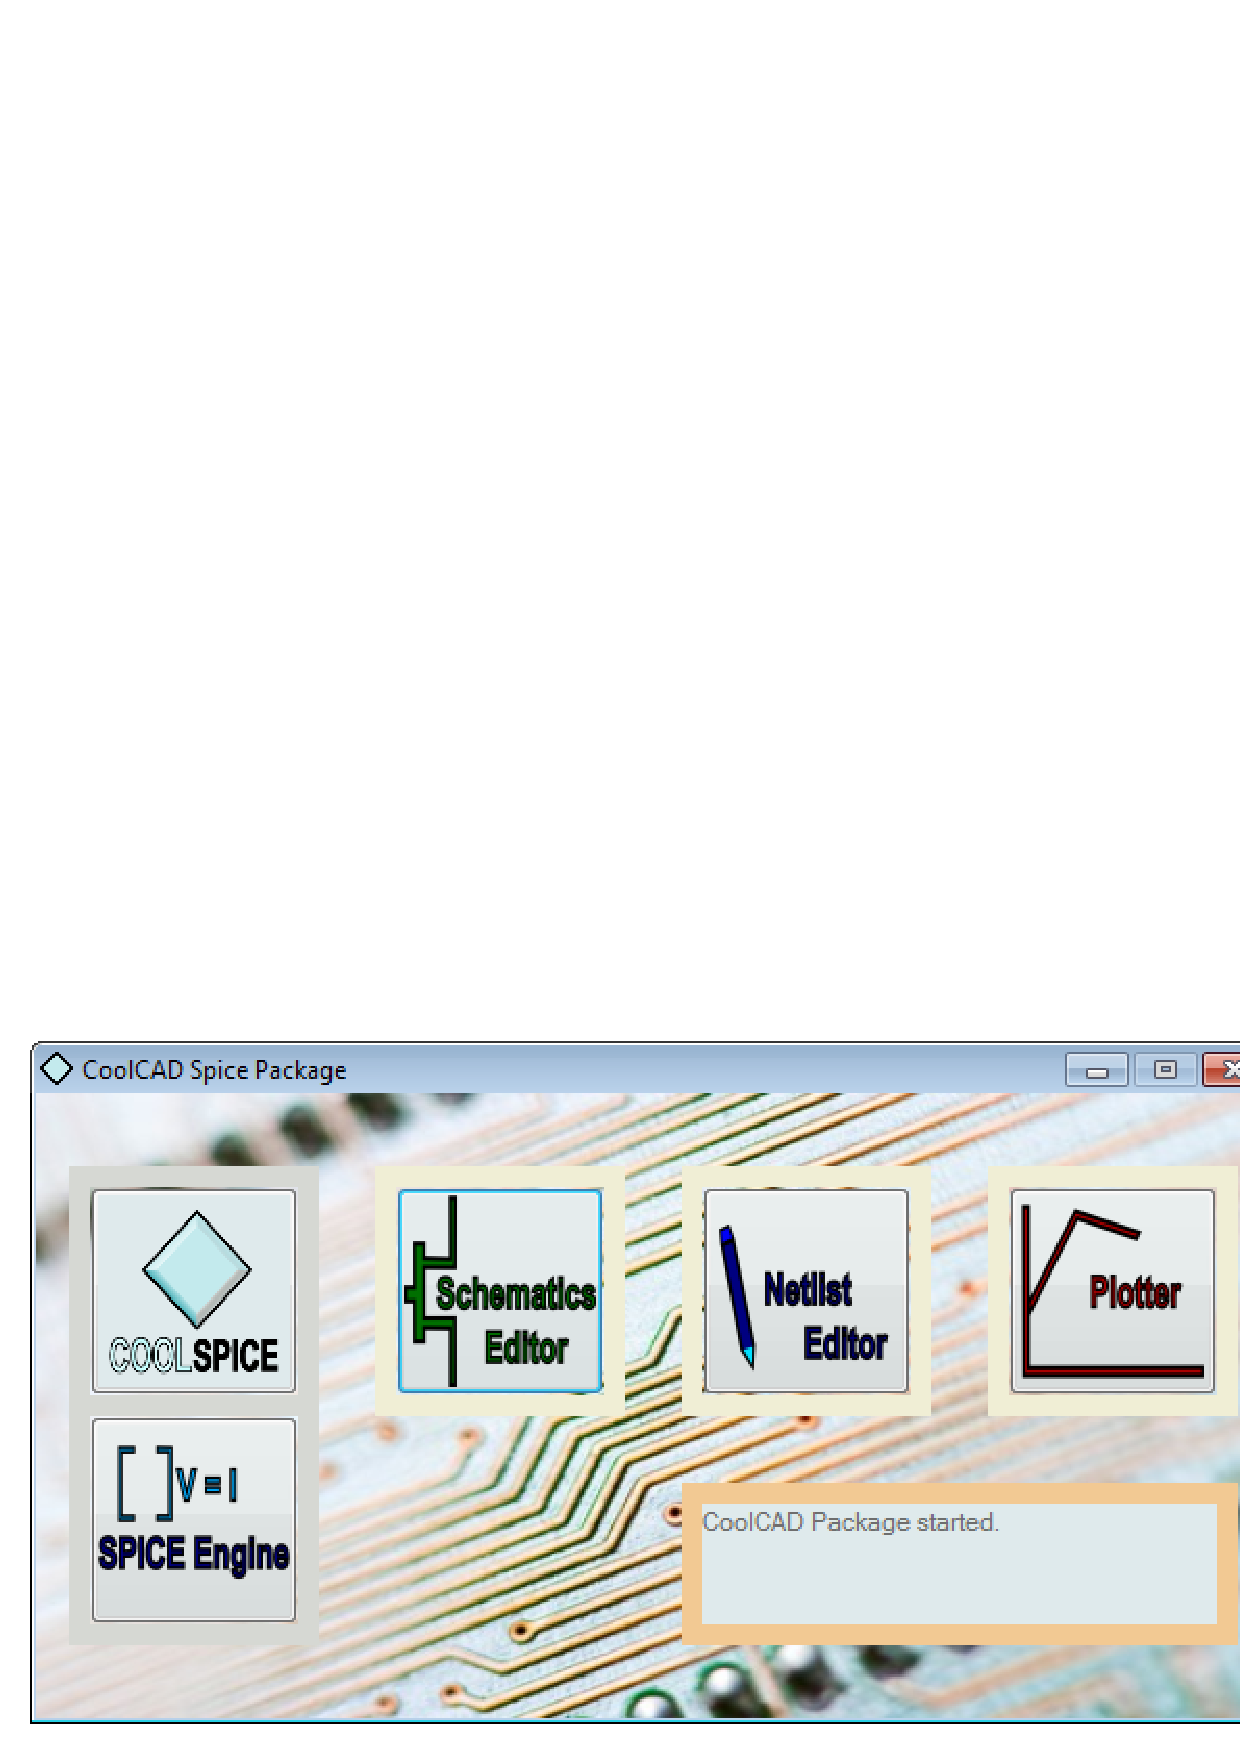
\includegraphics[width=0.55\textwidth]{./figures/getting_started_figures/CoolSPICE_mainconsole.png}
	\caption{{The main console of the CoolSPICE package.}}
  \label{fig_mainconsole}
\end{SCfigure}


\subsection{Building a Circuit}

On the main console, click on \textbf{Schematic Editor} to launch the Schematic Editor. By default, the Schematic Editor should open with frames which show the libraries and the selected symbol (when one is selected) to the left.  If these frames are not visible, click the \menuorbutton{Symbol Picker} button, which has the symbol \fbox{$\Omega$} (or press \makekey{F6}).  

For a fast-start example, we are going to build an inverter using the ON Semiconductor 0.5 $\mu$m technology and run a simulation to find its voltage and current transfer functions.  The MOSFET models are included in the built-in libraries of CoolSPICE.  Click on the ``+" symbol next to the MOSIS library to open up the list of components in this library.

\begin{SCfigure}[5.0][hbt]
    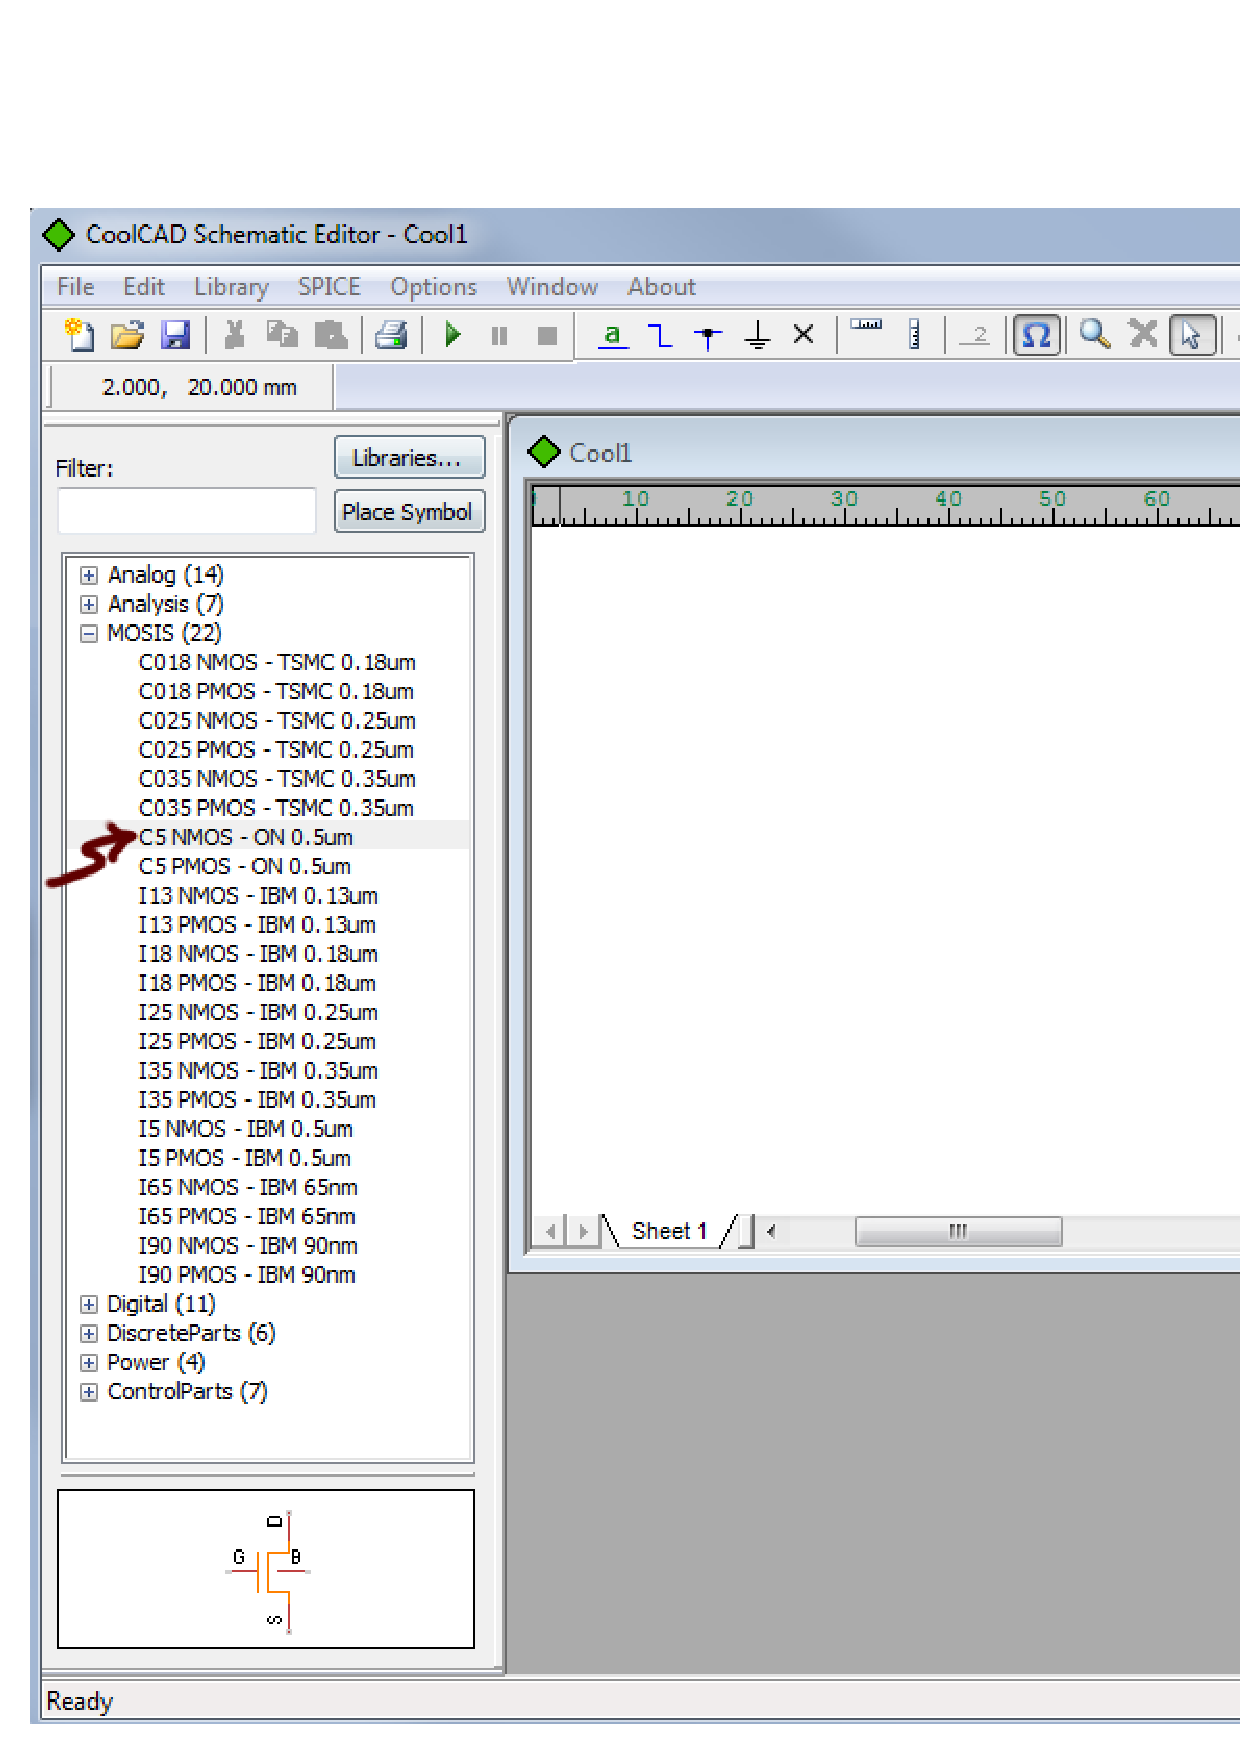
\includegraphics[width=0.55\textwidth]{./figures/getting_started_figures/CoolSPICE_emptySchematicEditor.png}
    \caption{{Schematic Editor with a model selected and ready.}}
  \label{fig_emptyschematiceditor}
\end{SCfigure}

\inserttip{Use the \textsf{\textsc{Esc}} key to cancel out of an action.} 

\mymarginnote{Inserting components} 
Double-clicking on the name of the required component (or single-clicking on the symbol which appears in the symbol frame) gives the user an instance of the component to place.  \index{Schematic Editor!component placement} It also opens up the \window{Options} for the component. \index{Schematic Editor!component options}  The user can place multiple instances of the same component until the place mode is cancelled by hitting the \textsf{\textbf{\textsc{Escape}}} key.  The \window{Options} disappears after the place mode is cancelled (or if the user clicks on an empty spot in the design area) and can be recalled by clicking on a component after placement.

\begin{SCfigure}[5.0][hbt]
    \includegraphics[width=0.55\textwidth]{./figures/getting_started_figures/CoolSPICE_SchematicEditorwithDevicesandOptions.png}
	\caption{{Schematic Editor with two components placed and the \textsf{Options} window.}}
  \label{fig_schematiceditor_devicesandoptions}
\end{SCfigure}

%\FloatBarrier
%\clearpage
%
\inserttip{Make sure all instances have distinct reference names. Avoid reference names with only numbers (e.g. ``42").} \mymarginnote{Component parameters} The component parameters can be changed by clicking on the value of the parameter in the \window{Options}.  As shown in Fig. \ref{fig_schematiceditor_changePMOSwidth}, here the width for the PMOS has been changed to 4.5 $\mu$m (by typing {\bf{\textsf{4.5u}}}).  The placement orientation and the instance reference name (\textbf{``Ref"}) for a component can also be changed from the \window{Options}.  

Note that if \textbf{``Ref"} is set to end with a number (e.g. ``D42"), when more instances of the same component are placed in the schematic by copy-paste, this reference number can automatically be incremented.  \emph{However, if the user edits the reference in the} {\textsf{Options}} \emph{box in between placements and places further instances, the reference number will} not \emph{be incremented} until the user cancels out of the action and restarts by copy-pasting or selecting the left-frame representation of the symbol to create a new instance.  This can lead to netlist conflicts. 

\begin{SCfigure}[5.0][t!]
    \includegraphics[width=0.55\textwidth]{./figures/getting_started_figures/SchematicEditor_ChangePMOSWidth.png}
    \caption{Changing component parameters using the \window{Options}.}
  \label{fig_schematiceditor_changePMOSwidth}
\end{SCfigure}

\begin{SCfigure}[5.0][hbt]
    \includegraphics[width=0.55\textwidth]{./figures/getting_started_figures/SchematicEditor_addingVDD.png}
    \caption{{Adding the VDD net pin.}}
  \label{fig_schematiceditor_addVDD}
\end{SCfigure}

\mymarginnote{Power and\\ground nets} We need to add power and ground nets and voltage sources. To add the pins for the power net, we use the \menuorbutton{Power} button (marked with the earth ground symbol) or press \makekey{F4}.  The net name is set in the dialogue box; symbol rotation and type are set by the radio buttons.  Figure \ref{fig_schematiceditor_addVDD} shows the VDD pin being added. \index{Schematic Editor!power nets} For the ground net, there are two options: \index{Schematic Editor!ground net} If the \menuorbutton{Power} button option is used, the pin \textit{must} be named ``\textbf{0}", which is in fact the default name; the other option is to use the ``\textbf{Source - Ground}" component in the \textbf{Analog} library, \index{Components!ground net} as in this example circuit (see Fig. \ref{fig_schematiceditor_wiredtogether}).   \index{Schematic Editor!ground nets}

\mymarginnote{Voltage\\sources} The voltage sources are also available under the Analog library. For this example we use DC voltage sources, labelled ``SourceV - DC AC" in the program.  Figure \ref{fig_schematiceditor_wiredtogether} shows the placement, naming and parameters of these DC sources. 

%\pagebreak
\mymarginnote{Adding\\ wires} Wires are added using the \menuorbutton{Wire} button (see Fig. \ref{fig_schematiceditor_wiredtogether}) or the \makekey{F2} hotkey. \index{Schematic Editor!wiring} Click to start the wire and once in the path to turn a corner.  (The first corner-turn in a given path is also detected from the mouse movement.) The wire angle can be set in the \dial{Wire Options}.  Double-clicking after a straight extension or right-clicking at any time ends the piece.  When the wire crosses another wire, a circle appears to present the option of forming a connection with a single click.  A connection also ends the wire segment. Figure \ref{fig_schematiceditor_wiredtogether} shows the wired circuit just before the last connection is placed. (Note that the mouse scroll button or the PgUp/PgDown keys zoom in/out. This is a zoomed-in figure. The user can also pan around the design by right click-hold-dragging the mouse.)  
\begin{SCfigure}[3.0][hbt]
    \includegraphics[width=0.55\textwidth]{./figures/getting_started_figures/SchematicEditor_addingwires.png}
    \caption{{Wired circuit.}}
  \label{fig_schematiceditor_wiredtogether}
\end{SCfigure} 


%\FloatBarrier
%\clearpage
%\newpage
%
\subsection{Analyses, Simulation and Viewing Results}

\inserttip{Do not label the net connected to the ground node or a power pin (e.g. VDD).\\Do not rely on capitalization to distinguish nets.} \mymarginnote{Labelling\\ nets} In order to measure and plot voltage signals, nets can be labelled with the Label tool (the button marked \fbox{\underline{a}}, or the \makekey{F1} hotkey).  \index{Schematic Editor!probes} For current signals, a current meter should be used.  The current meter is in the Analog library as ``Probe - Ammeter".  Figure \ref{fig_schematiceditor_sensetools} shows these elements in place and the input and output nets being labelled with \textsf{``Vin"} and \textsf{``Vout"}.  Note that the net names are \textit{not case-sensitive}. In SPICE, a net named \textsf{VGS} and one named \textsf{vgs} are the same in the netlist and if they are electrically different nets in the circuit, conflicts and errors will arise. \index{Naming nets} 

\mymarginnote{Defining\\analyses} The SPICE analysis tools are in the \textbf{``Analysis"} library.  For this example we use the \textsf{\textbf{.dc}} analysis. \index{SPICE!statements!.dc} \index{DC analysis} \index{Schematic Editor!SPICE analyses} Figure \ref{fig_schematiceditor_analysistool} shows the DC analysis setup in place.  Note especially how the voltage source to be swept is specified as ``Voltage Source1".  In this case, the common gate of the MOSFETs is being swept from 0 to 3V (the rail voltage) in 0.05V increments.

%\begin{figure}[b]
  %\centering
    %\includegraphics[width=0.55\textwidth]{./figures/getting_started_figures/SchematicEditor_labeling_and_Isense.png}
    %\caption{Inverter with input/output net labels and a current meter at the PMOS source.}
  %\label{fig_schematiceditor_sensetools}
%\end{figure} 

\begin{SCfigure}[5.0][ht]
    \includegraphics[width=0.55\textwidth]{./figures/getting_started_figures/SchematicEditor_labeling_and_Isense.png}
    \caption{Inverter with input/output net labels and a current meter at the PMOS source.}
  \label{fig_schematiceditor_sensetools}
\end{SCfigure} 

\mymarginnote{Saving and running} To run the analysis we first need to save the design.  The \menuorbutton{Save} button (floppy disk symbol) or the \menuitem{File}{Save} can be used.  To start the simulation, use the \menuorbutton{Run} button  (the ``play" symbol) or the \menuitem{SPICE}{Create Spice Net List and Run}.  This will create the netlist and ask for the netlist filename.  Here we use the same name as the design, \textsf{\textbf{inverter\_test1}}.  Just to see the netlist without running the simulation, use \menuitem{SPICE}{View SPICE Netlist}.  (The netlist is not editable from this view.)

\begin{SCfigure}[5.0][ht]
    \includegraphics[width=0.55\textwidth]{./figures/getting_started_figures/SchematicEditor_DCrunadded.png}
    \caption{{DC sweep specification.}}
  \label{fig_schematiceditor_analysistool}
\end{SCfigure} 


%\FloatBarrier
%
Under the \menuitem{SPICE}{Preferences}, {CoolSPICE} can be set to automatically launch the Plotter and/or show the simulation Log File and raw data file after the simulation is complete.  By default, the "Launch Plotter" option is enabled and the options to show log/raw data file are disabled. 

\inserttip{The model paths are relative! Watch where the netlister is searching for the model cards.}\mymarginnote{Simulation\\failures due\\to path error} A common cause for simulation failure is the path specification errors for the models.  CoolSPICE comes with built-in example circuits under the folder \textsf{CoolSpice/Ckts}, symbol libraries under \textsf{Libraries/} and model cards under \textsf{Models/}.  During netlist creation, the netlister looks for the models in the \textsf{../Models/} folder (\textit{i.e.} it expects the \textsf{Models/} folder to be one level up from the circuit itself) unless the models are edited to point at an alternative location.  If the path is not where the program searches, the simulation will fail, quietly if the user has not changed the SPICE preferences to show the logfile automatically.  (If the Plotter has been set to launch automatically, a window will warn that no raw data file was found.) As shown in Fig. \ref{fig_schematiceditor_logfileerror}, the log file (which is stored in the same folder as the circuit) displays where the netlister looked for the model file.  To avoid this problem, save the designs either in the \textsf{CoolSpice/Ckts/} folder (which is created by default) or in a folder at the same path level, such as \textsf{CoolSpice/MyCircuits/}. 

\begin{SCfigure}[5.0][t]
    \includegraphics[width=0.55\textwidth]{./figures/getting_started_figures/SchematicEditor_modelswrongplace.png}
    \caption{Error recorded in the log file if the model for devices in the circuit are not found where expected.}
  \label{fig_schematiceditor_logfileerror}
\end{SCfigure} 

\mymarginnote{Adding\\ a trace} After the simulation is complete, the CoolCADPlotter window \index{Plotter} is automatically launched if the option is enabled as it is by default.  To view results, click the \menuorbutton{Add Trace} button (see Fig. \ref{fig_plotter_addingtraces}) or use the \menuitem{Graph}{Add Traces}. \index{Plotter!adding traces}  The only option the software will present in this example is the current trace from the current probe, as seen in the figure.

\begin{SCfigure}[5.0][ht]
    \includegraphics[width=0.55\textwidth]{./figures/getting_started_figures/Plotter_addingtrace.png}
    \caption{Adding traces to the plotter.}
  \label{fig_plotter_addingtraces}
\end{SCfigure} 

%\FloatBarrier
%\clearpage
%
\mymarginnote{Setting trace\\ and view properties, navigating} Right-clicking on the plotting area allows the user to set properties of the trace (such as color and style), move traces between panels, make measurements or use other trace tools.  Right-clicking and dragging in the plotting area pans around the plot.  \index{Plotter!trace properties} \index{Plotter!ploto navigation} Single-clicking on an axis allows the user to set axis properties such as the label, ranges and step size. \index{Plotter!axis properties} Click-and-dragging to create a rectangle in the plotting area zooms in on that area.  Double-clicking on the trace-label box which displays the trace color and name zooms out to the full trace.   Right-clicking on the trace-label box opens the trace properties. When there are multiple traces, clicking on a trace name in the legend box makes it the active trace for measurements.  When there are multiple panes, a blue frame marks the active pane.

\begin{SCfigure}[5.0][h]
  \includegraphics[width=0.55\textwidth]
	{./figures/getting_started_figures/SchematicEditor_voltageprobeadded.png}
  \caption{A voltage probe connected to the \textsf{Vout} net.}
  \label{fig_addvoltageprobe}
\end{SCfigure}

For voltage transfer function, we add a voltage probe to the schematic (the \textsf{Probe - Voltmeter} component under the Analog library) connected to the line labeled \textsf{Vout}, as shown in Fig. \ref{fig_addvoltageprobe}.  After re-running the simulation, we can now add both traces and view the current and voltage transfer functions of the inverter.  Figure \ref{fig_plotter_bothtraces} shows the Plotter window when both traces have been added.  Since one trace is from a current meter and the other from a voltage meter, they are by default plotted on separate y-axes.  Note that the legend insets can be grabbed and moved by the mouse, as was done in this example since by default they blocked the low-input-voltage part of the voltage transfer function. 

\begin{SCfigure}[5.0][h]
    \includegraphics[width=0.55\textwidth]{./figures/getting_started_figures/Plotter_twotraces.png}
    \caption{The Plotter displaying two traces.}
  \label{fig_plotter_bothtraces}
\end{SCfigure} 

Another simulation example is given in Figure \ref{fig_transientsimexample}, where a one-stage common-source amplifier is simulated with \textsf{.tran} (transient) analysis.  Note that not $V_{in}$ but $V_{in}-1.25$ is displayed, so that the DC offset at the gate is removed to make reading the graph easier.  This is achieved using the \menuorbutton{Calculator} tool in the Plotter.

\begin{figure}[hbt]
\centering
  \includegraphics[width=0.55\textwidth]
	{./figures/getting_started_figures/CoolSPICE_examplesimulation_transient.png}
  \caption{A basic common-source amplifier simulated using transient analysis.}
  \label{fig_transientsimexample}
\end{figure}

The last example here in Figure \ref{fig_acsimexample} is the same CS amplifier subjected to a frequency-domain analysis using the \textsf{.ac} analysis tool.  Since the \textsf{.ac} tool in SPICE requires an AC source, note that the \textsf{SourceV - Sinewave} element in Fig. \ref{fig_transientsimexample} has been replaced with a \textsf{SourceV - DC AC} element in the new circuit.  The Plotter automatically plots the magnitude and phase of the selected traces, which allows the designer to evaluate the frequency domain characteristics of the circuit.

\begin{figure}[hbt]
\centering
  \includegraphics[width=0.55\textwidth]
	{./figures/getting_started_figures/CoolSPICE_examplesimulation_ac.png}
  \caption{A basic common-source amplifier simulated using ac analysis.}
  \label{fig_acsimexample}
\end{figure}

%\FloatBarrier
%
\subsection{Example Circuits}

Under the folder \textsf{CoolSpice/Ckts/} there are example circuits which are bundled with the program.  Running and playing around with the designs and SPICE analysis statements in these circuits is a good way to rapidly learn more about CoolSPICE and its capabilities.  As an example, Fig. \ref{fig_examplecircuitrunresult} shows the example circuit \textsf{IV\_IDVDM}, a circuit designed to run $I_{D}$-$V_{DS}$ sweeps on an TSMC 0.18 $\mu$m NMOS with $V_{GS}$ as a parameter.  Once the simulation is run as it is in the example, the curve \textsf{i\_vimeter} is available to  view in the Plotter.

\begin{figure}[hbt]
\centering
  \includegraphics[width=0.55\textwidth]
	{./figures/getting_started_figures/CoolSPICE_examplecircuit_IV_IDVDM.png}
  \caption{The example circuit \textsf{IV\_IDVDM} found in the \textsf{Ckts/} directory and its run results.}
  \label{fig_examplecircuitrunresult}
\end{figure}

%\FloatBarrier
%\clearpage
%
\subsection{Creating a New Symbol for Hierarchical Designs}
\label{subsec_iags_newsymbol}

To include a circuit or subcircuit in another schematic, a symbol needs to be associated with this circuit or subcircuit. \index{Schematic Editor!new symbol creation} In this example we design the symbol for the inverter circuit.  

The \menuitem{SPICE}{Add hierarchical symbol} opens another tab in the design window.  \mymarginnote{Polygon tool}  The original circuit remains on a tab named ``Sheet 1" by default.  The polygon tool, marked in Fig. \ref{fig_schematiceditor_symbol1}, can be used to draw lines and shapes.  The ellipse, rectangle and arc tools are also available in buttons next to the polygon tool. When using the polygon tool, right-click and choose \textsf{``Finish polygon"} to stop drawing. \index{Schematic Editor!drawing tools}

\begin{figure}[hbt]
\centering
  \includegraphics[width=0.55\textwidth]
	{./figures/getting_started_figures/SchematicEditor_drawingsymbol1.png}
  \caption{Creating an inverter symbol using the hierarchical symbol definition tool in the Schematic Editor.}
  \label{fig_schematiceditor_symbol1}
\end{figure}

\mymarginnote{Adding\\ symbol pins} The design itself should have labels on all the nodes which will correspond to pins in the symbol.  We first revise the design to take out the DC analysis command and the sources, since the VDD and ground pins of the inverter symbol would presumably be connected to sources in the circuit into which the inverter symbol is inserted.  Figure \ref{fig_schematiceditor_symbolandcircuit} shows, on the left, the revised circuit (note the new net names for VDD and ground) and, on the right, the corresponding symbol pins being added. \index{Schematic Editor!symbol pins} The pins are added with the \menuorbutton{Add Symbol Pin} button as marked in the figure.  Before clicking to place a pin, define the pin name, direction, graphical type and electrical type with the dialogue box.  Make sure that the electrical type fits what each pin needs to be for the circuit: In this example, \textsf{Vin} is an input pin, \textsf{Vout} is an output pin, and \textsf{VDD} and \textsf{cktgnd} are defined as input/output pins.  If unsure which type to use, it is best to pick ``input/output." 

\inserttip{Make sure to set reference names for the hierarchical symbols.}\mymarginnote{Hierarchical\\symbol\\references}Once the symbol has been saved, it can be incorporated into another circuit with the \menuitem{SPICE}{Insert another design as symbol...}. \index{Schematic Editor!using symbols}  The inverter circuit simulation results from Section are replicated using this new inverter symbol in Fig. \ref{fig_usingsymbolincircuitexample}.  Note that the reference names for inserted hierarchical symbols are \textsf{not} set automatically; nor are they incremented if you copy-paste a symbol to create multiple instances.  Set a distinct reference name for each symbol instance to avoid netlist errors.

\begin{figure}[th]
  \centering
    \includegraphics[width=0.55\textwidth]{./figures/getting_started_figures/SchematicEditor_revisedcircuitandsymbol2.png}
    \caption{The inverter circuit revised for representation as a hierarchical symbol (left) and pin definition in the symbol view (right).}
  \label{fig_schematiceditor_symbolandcircuit}
\end{figure} 

\begin{figure}[hbt]
  \centering
    \includegraphics[width=0.55\textwidth]{./figures/getting_started_figures/CoolSPICE_invertersymbolincircuitexample2.png}
    \caption{The inverter symbol used in a simulation.}
  \label{fig_usingsymbolincircuitexample}
\end{figure} 

%\FloatBarrier
%\clearpage
%\newpage
%
\subsection{Creating New Component Models and Libraries}

In the Schematic Editor, users can access existing libraries to edit them, or add new component libraries, by the \makebutton{Libraries...} button at the top of the left-side frame (see Fig. \ref{fig_schematiceditor_accessinglibraries}). \index{Schematic Editor!component libraries!adding new components} This opens the \window{Library Setup}.  In this window, double-clicking a library or selecting it and clicking the \makebutton{Edit} button opens the symbol list for this library.  There, the user can right-click on an existing symbol to edit the symbol or perform other operations. \index{Component libraries!editing} \index{Component libraries!new library}

\begin{figure}[htb]
  \centering
    \includegraphics[width=0.55\textwidth]
		{./figures/getting_started_figures/SchematicEditor_openinglibraries.png}
    \caption{The \colorbox{lightgray}{\textcolor{black}{\textsf{\textbf{Libraries...}}}} button displays libraries and allows new ones to be created.}
  \label{fig_schematiceditor_accessinglibraries}
\end{figure} 

\mymarginnote{Creating a\\new library\\and adding\\a new\\component} As an example, we will create a new library and populate it with a new diode model.  The \makebutton{New} button in the \window{Library Setup} opens a \dial{Save As...}  for the user to set the location and name for the new library.  In this example, the library \textsf{testlibrary1.TCLib} is created and saved in a folder named \textsf{MyLibraries/} under the \textsf{CoolSpice} folder. \index{Component libraries!editing} \index{Component libraries!location} This sends the user back to the \window{Library Setup} with the new library added to the list.

We will base the new diode on the symbol and part statement of an existing diode in the \textbf{``DiscreteParts"} library. Double-clicking this library brings up the devices it contains.  Right-clicking on the \texttt{1N4148} diode, we choose \menuorbutton{Copy to}$\to$\menuorbutton{...} and pick the new library we created, as shown in Fig. \ref{fig_schematiceditor_copysymboltolibrary}.  This brings up the \dial{Update Library Symbol} box, showing the properties of the symbol just copied into the new library.

\begin{SCfigure}[5.0][bt]
  \includegraphics[width=0.55\textwidth]
	{./figures/getting_started_figures/SchematicEditor_copymodeltonewlibrary.png}
  \caption{An existing diode model is copied from the \textsf{DiscreteParts} library to the newly-created \textsf{testlibrary1} library for easy use of the symbol and the part statement.}
  \label{fig_schematiceditor_copysymboltolibrary}
\end{SCfigure}


As seen in Figure \ref{fig_schematiceditor_updatelibrarysymbol}, \textsf{Update Library Symbol} is where the attributes and associated SPICE model for components are defined.  For existing components, this window is launched by right-clicking on the symbol and choosing  \menuorbutton{``Symbol Properties..."}.  For the new component, first click on the value of the \textsf{Name} parameter and give the new name.  (Hit \menuorbutton{Tab} or \menuorbutton{Enter} for the value to be reflected in the left-side frame.)  Note that the \textsf{Reference} parameter is set as \textbf{D} since our example device is a diode.    

\begin{SCfigure}[5.0][bt]
  \includegraphics[width=0.55\textwidth]
	{./figures/getting_started_figures/SchematicEditor_UpdateLibrarySymbol.png}
  \caption{The name, description and other attributes of the new component are defined in the \menuorbutton{Attributes} tab of the \textsf{Update Library Symbol} {window.}}
  \label{fig_schematiceditor_updatelibrarysymbol}
\end{SCfigure}

Under the \textsf{SPICE} tab, the \textsf{``Model"} box is used to define the default \textit{part statement} the netlister uses to generate the SPICE netlist line when encountering this component. \mymarginnote{Specifying \\a device\\ model card} The \textsf{``Prologue"} or \textsf{``Epilogue"} boxes are used to define the \textsf{.include} statement which points to the model card. \index{SPICE!statements!.include} It is necessary to fill only one of these two; the netlister puts the \textsf{.include} statement either to the very beginning or the very end of the netlist depending on which one has been used.  Since we copied a diode component, we do not need to edit anything in the \textsf{Model} box part statement except the model name (see Fig. \ref{fig_schematiceditor_definingmodel}). 

\begin{SCfigure}[5.0][bt]
  \includegraphics[width=0.55\textwidth]
	{./figures/getting_started_figures/SchematicEditor_enteringthemodel.png}
  \caption{The part statement and \textsf{.include} statement pointing to the file which includes the \textsf{.model} statement for the device are defined in the \textsf{SPICE} tab of the {\textsf{Update Library Symbol}} window.}
  \label{fig_schematiceditor_definingmodel}
\end{SCfigure}

The model name should match the model card (\textsf{.model} statement) in the text file specified by the \textsf{.include} statement in the \textsf{Prologue} or \textsf{Epilogue} box.  For this example, the contents of the text file {\textsf{../Models/ExtraParts.txt}} have been reproduced below.
\vspace{\parskip}

\noindent\begin{minipage}{\textwidth}
\begin{center}\small{
\texttt{.model TestDiode  D(Is=5.84n N=1.94 Rs=.7017 Ikf=44.17m Xti=3 
Eg=1.11\\+Cjo=.95p M=.55 Vj=.75 Fc=.5 Isr=11.1n Nr=2.09 Bv=100 Ibv=100u Tt=11.1n)}}
\end{center}
\end{minipage}
\inserttip{Note that the model name (\texttt{TestDiode}) specified at the end of the part statement in the \textsf{Model} box in Fig. \ref{fig_schematiceditor_definingmodel}.} 

Click \makebutton{Store} to save the symbol attributes and SPICE information and return to the symbol display window. The new component can now be used in the Schematic Editor. The new library appears in the library list and includes and the new component (See Fig. \ref{fig_schematiceditor_newdeviceavailable}). 

Another method to specify the component SPICE model is to write out the \textsf{.model} statement in the \textsf{Prologue} or \textsf{Epilogue} dialog box instead of putting it in a text file and pointing to the file with a \textsf{.include} statement as above.  However, the \textsf{.include} method has the advantage that it is possible to incorporate more than one \textsf{.model} statement in a text file.  Then, when defining the models for multiple components within the same library, the same \textsf{.include} statement works for all. This helps with organization.  For instance, Fig. \ref{fig_schematiceditor_mosfetcopyexample} shows another new device, this time a MOSFET, defined in the same library by the copying method described above.  For it to work correctly, the file \textsf{../Models/ExtraParts.txt} should now also include an NMOS \textsf{.model} statement with the model name ``generic018nmos."

It is also possible to edit existing libraries, point existing models to new \textsf{.model} statements \textit{etc.} by starting with the \makebutton{Libraries} button as above. \mymarginnote{Editing\\existing\\component\\models}However,  note that if the model for a component with existing instances in the design is changed, either by pointing it to a new model card file by editing the \textsf{.include} statement or by editing the \textsf{.model} statement in the model card text file, \textit{only new instances of it will use the new model in the netlist.}  Existing instances will have to be deleted and replaced to be associated with the modified model. \inserttip{The netlist creator does not check if models are up to date with existing instances of components! If you changed a model, replace the instances to apply the change to everything.}  

% \vfill
% \clearpage
% \pagebreak

\begin{SCfigure}[5.0][th]
	\includegraphics[width=0.25\textwidth]
	{./figures/getting_started_figures/SchematicEditor_NewLibraryDeviceAvailable.png}
  \caption{The new library and component (with its symbol and model) are now available for use in schematics.}
  \label{fig_schematiceditor_newdeviceavailable}
\end{SCfigure}

\begin{SCfigure}[5.0][bh]
	\includegraphics[width=0.7\textwidth]
	{./figures/getting_started_figures/SchematicEditor_MOSFETmodelexample.png}
  \caption{The part statement for a MOSFET defined in the new library by copying the MOSFET symbol from the MOSIS library.}
  \label{fig_schematiceditor_mosfetcopyexample}
\end{SCfigure}

%\FloatBarrier
%\newpage
%\pagebreak
%\clearpage
%
\section{References and Further Reading}

\begin{enumerate}

\item CoolCAD CoolSPICE, http://coolcadelectronics.com/coolspice/, last visited October 2014.

\item WinSCP, http://winscp.net, last visited October 2014.

\item List of SPICE device codes, http://www.ecircuitcenter.com/SPICEsummary.htm\#devices, last visited October 2014.


\end{enumerate}

\chapter{The Schematic Editor}

CoolCAD Schematic Editor is the schematic capture tool for the CoolSPICE suite.  It comprises symbol and analysis tool libraries, symbol placement and wiring tools, and drawing tools with a built-in symbol editor for the design of new symbols.  The designer can create the SPICE netlist from the schematic and automatically invoke the CoolCAD SPICE engine to run the simulation from within the Schematic Editor.

Quick references to the tool buttons available in the Schematic Editor can be at the end of this Chapter.

\section{Drawing a Circuit}

By default, the Schematic Editor opens with an empty schematic named ``Cool1" in an inset window.  The inset windows can be closed, maximized to cover the full Schematic Editor ``desktop," or minimized.  A new window is opened by the \menuitem{File}{New}. An existing design is opened by the \menuitem{File}{Open...}.

\mymarginnote{Schematic \\navigation} The mouse scroll button can be used to zooming in or out of the schematic.  Clicking and holding the scroll button (or the middle button in a three-button mouse) can be used to pan around the schematic.

\subsection{Component Placement and Options}
\label{subsec_se_componentplacement}

Components are inserted by using the \textsf{Symbol Picker} frame, which is visible by default on the left-side of the Schematic Editor window and can be toggled on/off using the \menuorbutton{Symbol Picker} button (\fbox{$\Omega$}, see Fig. \ref{fig_schematiceditor_changePMOSwidth}).  The panel libraries can be expanded using the \fbox{+} buttons.  

Double-clicking a component name, or single-clicking and pressing the \makebutton{Place Symbol} button, or single-clicking the symbol representation in the frame underneath the library list, puts Schematic Editor in placing mode.  Multiple copies of a symbol can be placed by clicking consecutively in new locations.  

As with any action in the Schematic Editor, the placing action can be cancelled by pressing the \makekey{\textsc{Esc}} key.

Components are selected individually by clicking once on the symbol placed in the drawing area.  This brings the \window{Options} back up.  Figure \ref{fig_schematiceditor_annotatedoptions} shows the different elements of the \window{Options}:

\mymarginnote{Options\\details}
\begin{itemize}
\item \textit{Orientation Options} allow the user to place the symbol in four cardinal orientations and as a mirror-image if desired.
\item \textit{The Reference Name}, which may be automatically assigned by the program or manually by the user, is the name that the netlister will use to reference the component in the netlist.  Note that unclicking the tickbox next to \textsf{Ref} \textit{only hides the reference name in the circuit view}; the netlister still uses the reference name to identify the component.
\item \textit{Show Power Pins} enables/disables the display of power pins.
\item \textit{Allow Re-Sizing} shows or hides a resizing box with which the user can resize the symbol to better suit the design need.
\item \textit{The Temperature Setting} sets the individual device temperature for temperature-dependent parameter calculation during simulation.  This has no effect in the Student Edition.
\item \textit{The} \makebutton{Show Model} \textit{Button} shows the model card associated with the symbol.  If this model card is defined within a text file with an \textsf{.include} statement (see Section \ref{sec_se_symbolsandlibraries}) the program will display the entire file.
\item \textit{The Parameters} change depending on the component type.  Some parameters are compulsory to define for simulation.  More information on component parameters can be found for analysis commands and analysis-related components such as probes, and for active and passive devices as well as behavioral devices.
\item \textit{The} \makebutton{Add} \textit{and} \makebutton{Delete} \textit{Buttons} allow the user to define a new parameter or remove it. This is useful for user-defined symbols detailed in Section \ref{sec_se_symbolsandlibraries}.
\end{itemize}

\begin{SCfigure}[5.0][hbt]
    \includegraphics[width=0.65\textwidth]{./figures/schematic_editor_figures/SchematicEditor_PartOptionsDialogue_Annotated.png}
    \caption{{The Options window for a \textsf{TSMC 0.18um C018 PMOS} from the \textsf{MOSIS} library.  See the text body for the annotations.}}
  \label{fig_schematiceditor_annotatedoptions}
\end{SCfigure}


Right-clicking on the schematic window brings up a contextual menu which allows the user to perform some actions on the selected component, such as rotation, copy/paste, or cut.  The first option in the contextual menu, \textsf{Replace Symbol...} allows the user to replace either only the selected symbol, or all instances of this symbol in the design, by another symbol which must first be selected by entering part of its name into the search box.


\subsubsection{Reference Name Assignment}

The program automatically increments names for new instances of a given {component} if:
\begin{itemize}
\item The user picks the component by double-clicking on the name in the library or single-clicking on the symbol representation and places multiple instances by repeated clicks in the circuit design area without altering the \textsf{Ref} box in the \window{Options}, or
\item The user selects an already-placed component and chooses \menuitem{Edit}{Copy} / \menuitem{Edit}{Paste} (or uses the \makekey{Ctrl}-\makekey{C} / \makekey{Ctrl}-\makekey{V} key combinations) to place new instances without altering the \textsf{Ref} box in the \window{Options}.
\end{itemize}

\mymarginnote{Name\\increment\\exceptions}However, the software will \textit{not} increment the name in the case that the user:
\begin{itemize}
\item ...picks the component by double-clicking its name in the library list or single-clicking the symbol representation, and edits the reference name in the \textsf{Ref} box \textit{before} placing the first instance, or 
\item ...edits the reference name in the \textsf{Ref} box in between placing further instances, or
\item ...selects an already-placed component and edits the reference name in the \textsf{Ref} box to a name which contains only numbers (\textit{e.g.} ``123"), then uses the copy-paste method to make further copies.
\end{itemize}These cases may result in instances of the same component with identical names, which will lead to netlist conflicts. 

\inserttip{It is very important to ensure that each component instance has a distinct Reference Name.  Do not use reference names comprising only numbers.}

Also note that if the user edits the reference name of one of the instances of the same type of component to something out of the sequence, then makes further copies of the component, the incrementer will continue incrementing from the lowest available number appended.  For instance, if the circuit has instances \textsf{N1} through \textsf{N5}, and the user edits \textsf{N5} to \textsf{N42} and then places more instances by copy-pasting from any of the present instances, the incrementer will continue from \textsf{N5}, not \textsf{N43}.

\subsection{Wiring and Labels}
\label{subsec_se_wiringandlabels}

To start laying out a wire, click the \menuorbutton{Wire} tool button (see Fig. \ref{fig_schematiceditor_wiredtogether}) or press \makekey{F2}. The \window{Options} allows you to set the wire angle.  The first turn in the wire segment will be detected by the program depending on the mouse movement.  Double-clicking after a straight extension or right-clicking at any time ends the piece. When the wire crosses another wire, a circle appears to present the option of forming a connection with a single click.  A connection also ends the wire segment. Figure \ref{fig_schematiceditor_wiredtogether} shows the wired circuit just before the last connection is placed.

\mymarginnote{Labelling} In SPICE netlists, wires appear as the circuit nodes they represent.  If the wires are not labeled in the schematic, the netlister will use an automatic numbering scheme.  Labelling gives netlists that are easier to read (and after simulation, makes it easier to identify which signals to look at).  The \menuorbutton{Label} button (\fbox{\underline{a}}) or the \makekey{F1} key is used to set labels.  Figure \ref{fig_schematiceditor_labelexample} shows the net \textsf{Vout} being labelled.  In the \window{Label Options}, the top row is used to select the orientation of the letters.  The red dot that appears with the label on the schematic shows the location of the label (the net contacting this dot will take on the label).  Once the label is placed, the user can write another label name in the dialogue box.  The \makebutton{Font} and \makebutton{Colour} buttons can be used to set the font and color of the label on the schematic.

\begin{SCfigure}[5.0][hbt]
    \includegraphics[width=0.65\textwidth]{./figures/schematic_editor_figures/SchematicEditor_LabelOptionsDialogue.png}
    \caption{{Labelling the node \textsf{Vout}.}}
  \label{fig_schematiceditor_labelexample}
\end{SCfigure}

With the labels, the MOSFET appears in the netlist with the following line:

\spicesyntax{\begin{tabular}{l}
MN1 Vdrain Vin Vs Vs on0p5nmos W=20u L=3u \\
\end{tabular} }

Whereas without the labels, the netlister automatically numbers the nodes:

\spicesyntax{\begin{tabular}{l}
MN1 \_N\_4 \_N\_8 \_N\_3 \_N\_3 on0p5nmos W=20u L=3u \\
\end{tabular} }

\subsection{Power Nets and Sources}
\label{subsec_se_powernetsandsources}

The power and ground nets are defined using inserted into the circuit using the \menuorbutton{Power} button (The "earth ground" symbol, see Fig. \ref{fig_schematiceditor_addVDD}) or pressing \makekey{F4}.  The name of the pin is entered using the dialogue box.   Different designs and orientations for the pin are available in the \window{Options}.

\inserttip{The ground pin name \textit{must} be \textbf{\texttt{0}}.} 

Multiple pins with the same name are used to denote the same node, which allows the user to avoid overly complicated wire networks in the schematic.  For an example, the netlist of the circuit shown in Fig. \ref{fig_schematiceditor_multiplepins} has the DC source \textsf{VS2} correctly wired between the away-from-drain end of the resistor \textsf{R1} and the ground.  For a circuit with multiple stages with drains all connected to \textsf{VDD}, this would cut down on the number of required wires.  This also enables multi-sheet designs, as described below in section \ref{sec_se_multisheetdesigns}.

\begin{SCfigure}[5.0][hbt]
    \includegraphics[width=0.4\textwidth]{./figures/schematic_editor_figures/SchematicEditor_MultiPinUseExample.png}
    \caption{{Using multiple copies of the same pin to clarify schematic design.  Each arrow-paired pair of marked dots are connected to the same node.}}
  \label{fig_schematiceditor_multiplepins}
\end{SCfigure}

\mymarginnote{Sources} The voltage and current sources are found under the \textsf{Analog} library.  The voltage sources are labeled ``\textsf{SourceV}" and current sources are labeled ``\textsf{SourceI}".  Details about the parameters of these components are found elsewhere. From the Schematic Editor the user can define DC/AC, Pulse (i.e. square wave) and Sinewave sources.  Other sources, such as the piecewise linear source, can be defined using the Netlist Editor.

\subsection{Probes}
\label{subsec_se_probes}

Inserting a current or voltage probe in the schematic directs the netlister to insert a \texttt{.save} statement in the netlist to store the branch current or node voltage results as appropriate for the proper analysis.  The probes are available in the Schematic Editor under the \textsf{Analog} library.  Naturally, current probes must be inserted into a branch and voltage probes connected to nodes.  Figure \ref{fig_transientsimexample} has an example circuit with a current probe measuring the drain current and three voltage probes measuring the gate, drain, and post-DC-filter output voltages.

\subsection{Further Navigation and Schematic Commands}
\label{subsec_se_morenavigation}

As mentioned above, one can use the mouse scroll button to zoom in and out of the design and the middle button/scroll button click-and-hold to pan around the circuit.  

Right-clicking anywhere around the drawing area brings up the contextual menu, which has a number of general commands and a number of selected-component-specific commands that are available.  (The selected-component-specific commands are greyed out unless the user right-clicks in the symbol area of a selected component.) Figure \ref{fig_schematiceditor_contextualmenu} shows the contextual menu invoked on the current meter \textsf{Imeter1} in the displayed circuit.

The \menuitem{Z-Order}{Bring to front} and \textbf{\textsf{Send to back}} commands in the contextual menu are useful for when images are imported into the Schematic Editor for use in a symbol or similar, as will be described in Section \ref{sec_se_hierarchicaldesigns}.  

It is possible to move the shown properties of components (including the reference names) to avoid conflicts and overlays.  In Figure \ref{fig_schematiceditor_contextualmenu} , the reference name \textsf{Voutmet1}, associated with the visible voltage probe, has been moved from its default location when the component is first set (which was directly above the visible \textsf{.op} line in the figure) by left-click and dragging on the text line.

\begin{SCfigure}[5.0][hbt]
    \includegraphics[width=0.6\textwidth]{./figures/schematic_editor_figures/SchematicEditor_ContextualMenu_MovingTextLabels.png}
    \caption{{The contextual menu comes up with a right-click in the schematic area.  If a device's symbol area is selected, the component-specific commands are enabled.  Also note that it is possible to move the reference name and property text for components, as for the case for the reference name of the voltage probe here.}}
  \label{fig_schematiceditor_contextualmenu}
\end{SCfigure}


\section{Multi-sheet Designs}
\label{sec_se_multisheetdesigns}

For complicated circuits, it is possible to split the circuit drawing into multiple sheets.  For a given design (\textsf{.dsn} file), the netlister will combine all sheets into a single circuit netlist.  Node and wire names should not be repeated between sheets except where a connection is explicitly intended, and the designer should take care that multiple components do not have the same reference name between sheets either.  

To start a new sheet, or to delete or rename a sheet, right click on the sheet tab at the bottom of the design window, which says \textsf{Sheet 1} by default when a circuit is first started.  

Use the power pins and wire labels to ensure correct connectivity between the circuit parts on different sheets.  For an example, Figure \ref{fig_schematiceditor_multisheetexample} shows a two-stage amplifier split into two sheets for illustration.  (While this is a circuit which could easily fit on a single sheet, the simplicity helps the example.)  The features to note here are how the drain-side voltage source for both transistors is defined on Sheet 1 as the voltage source \textsf{VS2} as described above in Section \ref{subsec_se_powernetsandsources}, how the gate, drain and source networks have distinguishing names between the two sheets, and how the DC-isolated output of stage 1, equivalently the DC-isolated input of stage 2, bears the same node name \textsf{Vout\_st1}. 

\begin{figure}[thb]
\centering
  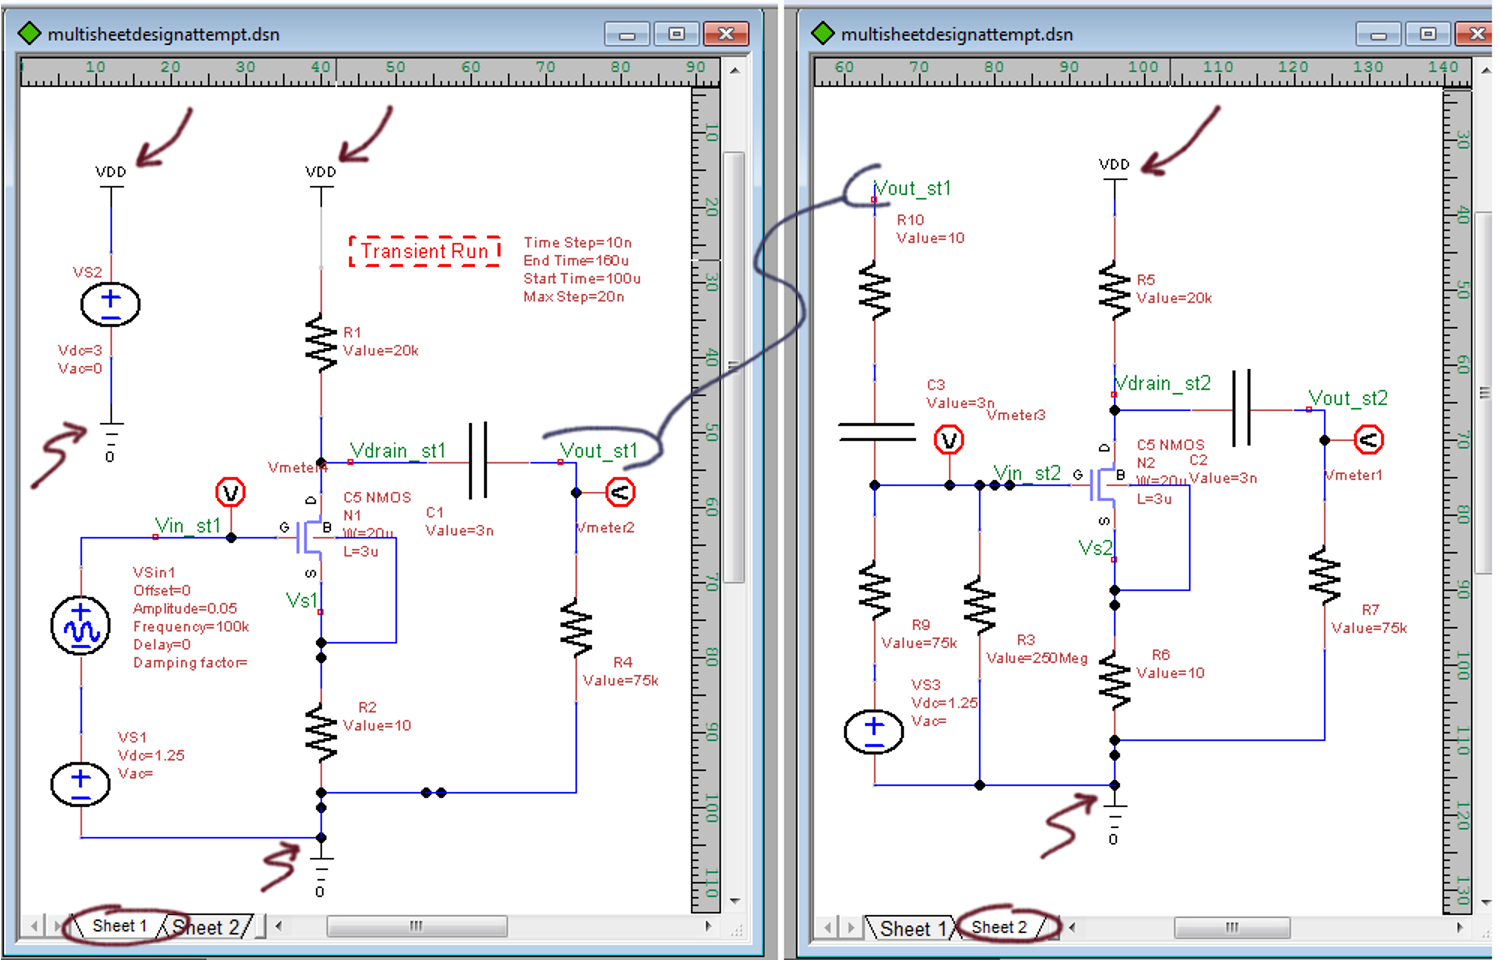
\includegraphics[width=0.97\textwidth]
	{./figures/schematic_editor_figures/SchematicEditor_MultiSheetDesign.png}
  \caption{A two-stage amplifier as an example of multi-sheet design.}
  \label{fig_schematiceditor_multisheetexample}
\end{figure}

Part of the netlist for this circuit is shown here:

\spicesyntax{\begin{tabular}{l}
CC1 Vout\_st1 Vdrain\_st1 3n \\
CC2 Vout\_st2 Vdrain\_st2 3n \\
CC3 Vin\_st2 \_N\_13 3n \\
MN1 Vdrain\_st1 Vin\_st1 Vs1 Vs1 on0p5nmos W=20u L=3u \\ 
MN2 Vdrain\_st2 Vin\_st2 Vs2 Vs2 on0p5nmos W=20u L=3u \\
RR1 Vdrain\_st1 VDD 20k \\
RR10 \_N\_13 Vout\_st1 10 \\
(...) \\
RR4 0 Vout\_st1 75k \\
RR5 Vdrain\_st2 VDD 20k \\
(...) \\
RR7 0 Vout\_st2 75k \\
(...) \\
VVS2 VDD 0   DC  3  AC  0   \\
.save v(Vout\_st2) \\
.save v(Vout\_st1) \\
.save v(Vin\_st2) \\
.save v(Vin\_st1)
\end{tabular}}

% \spicesyntax{\begin{tabular}{l}
% * Schematics Netlist * \\
% .include "../Models/MyMOS.txt" \\
% \\ 
% MN1\_x line\_out \_HN\_1\_Vin 0 0 nmos0p5 W=3u L=0.6u \\
% MP1\_x line\_out \_HN\_1\_Vin \_HN\_1\_VDD \_HN\_1\_VDD pmos0p5 W=4.5u L=0.6u \\
% VVG1 \_HN\_1\_Vin 0   DC  3         \\
% VVS1 VDD 0   DC  3     \\
% \\
% .dc VVG1 0 3 0.05   \\
% .end 
% \end{tabular} }


Note that the resistors \texttt{RR1} and \texttt{RR5} are the resistors between the two transistors' drains and \textsf{VDD}, and they are correctly shorted to the same node whose voltage is set by the voltage source \texttt{VVS2}.  When this circuit is netlisted and ran, all the traces from the four visible voltage probes will be saved and be available for plotting.

\section{Models and Libraries}
\label{sec_se_symbolsandlibraries}

\subsection{Symbols and Hierarchical Designs}
\label{sec_se_hierarchicaldesigns}

\section{Netlisting and Simulation}
\label{sec_se_netlistingandsimulation}

\subsection{OP Analysis}
\label{sec_se_opanalysis}

\section{Options and Preferences}
\label{sec_se_optionsandpreferences}

\section{Schematic Editor GUI Reference}
\label{sec_se_guiref}

\newpage
\begin{figure}[h]
  \centering
    \includegraphics[width=0.72\textwidth]
		{./figures/appendix_buttons_menus_figures/SchematicEditor_LeftButtons.png}
    \caption{Left-side buttons on the Schematic Editor.}
  \label{fig_schematiceditor_leftbuttons_inchapter}
\end{figure} 

\vspace{\parskip}
\begin{figure}[htb]
  \centering
    \includegraphics[width=0.72\textwidth]
		{./figures/appendix_buttons_menus_figures/SchematicEditor_RightButtons.png}
    \caption{Right-side buttons on the Schematic Editor.}
  \label{fig_schematiceditor_rightbuttons_inchapter}
\end{figure} 

A list of menu items for the Schematic Editor can be found in the Appendix.



\chapter{Plotter and Netlist Editor}

\label{chap_plotterandnetlisteditor_pane}

\section{Plotter}
\label{sec_pane_plotter}

The CoolSPICE Plotter is used to plot simulation results, stored in \textsf{.raw} files. These "rawfiles" are data files containing simulation results (node voltages and branch currents indicated by probes in the schematic, or by \texttt{.save} statements in the netlist).  These files have the same file name as the netlist or schematic, and are placed in the same directory by default.  

\subsection{Start-up and Loading Data}
\label{subsec_pane_startuploadingdata}

The plotter can be started from the main console by clicking on the \makebutton{Plotter} button.  Then using the \menuitem{File}{Open} (\makekey{Ctrl}-\makekey{O}, or the \makebutton{Open} button), the user loads a simulation result rawfile (\textsf{.raw} extension) and can plot the available traces stored in this file.  A file must be loaded first for traces to be available for plotting.

\inserttip{Rawfiles are plain text files allowing the user to view raw data directly.}

If the \textsf{Open Plotter} option is checked under the \menuitem{SPICE}{Preferences} of the Schematic Editor, the Plotter will start automatically at the completion of each successful simulation run, or an error message will pop up if the simulation did not complete successfully and write a \textsf{.raw} file.

\mymarginnote{Multiple subwindows} The Plotter window can be divided into multiple inset windows the same way as the Schematic Editor can be, by using the subwindow minimize/part window/close buttons (marked as ``subwindow control windows" in the figure in Section \ref{subsec_pane_plotterguireference}).  To create a new subwindow, simply load a new rawfile as described above and use the subwindow control buttons to minimize and arrange buttons.  Fig. \ref{fig_plotter_multiplesubwindows} in the shows an example of signals from two separate rawfiles being plotted.


\begin{SCfigure}[5.0][hbt]
    \includegraphics[width=0.6\textwidth]{./figures/plotter_netlist_editor_figures/Plotter_MultipleSubwindows.png}
    \caption{{Signals from two designs plotted in the same main Plotter window.}}
  \label{fig_plotter_multiplesubwindows}
\end{SCfigure}

\subsection{Adding Panes and Traces, Editing Traces}
\label{subsec_pane_addingtraces}

The Plotter window can be subdivided into multiple ``view"s and each "view" can be further subdivided into multiple panes. Each pane can be used to plot one or more traces. To split a pane and create a new pane, use the \textsf{Split Pane} button (see Fig. \ref{fig_plotter_multipaneaddtrace} and the annotated figures in Section \ref{subsec_pane_plotterguireference}) or the \menuitem{View}{Split Pane}. The active pane is highlighted with a blue border as shown in the figure.  Operations such as adding and removing traces are performed in the active pane, which can be selected by left-clicking in the pane area.   

\begin{SCfigure}[5.0][hbt]
    \includegraphics[width=0.6\textwidth]{./figures/plotter_netlist_editor_figures/Plotter_AddingTraces_MultiPane.png}
    \caption{{Two panes created on a plot window in which the file \textsf{Cir\_CommonSourceBipolar.raw} has been loaded.  The trace \textsf{v\_vin\_} has already been plotted on the top trace.  The bottom trace is the currently active one, into which the user is adding \textsf{v\_ac\_probe\_out\_} to plot.  The Add Trace and Split View buttons are marked by a circle and an arrow, respectively.}}
  \label{fig_plotter_multipaneaddtrace}
\end{SCfigure}

To add a trace, use the ``Add Trace" button from the button panel (see Fig. \ref{fig_plotter_multipaneaddtrace} and the annotated figures in Section \ref{subsec_pane_plotterguireference}), the \menuitem{Graph}{Add Traces}, or right-click on the active panel and choose \textsf{Add New Trace} from the contextual menu. A list of the saved traces from the loaded rawfile (or from the recent simulation, if the Plotter was initiated from a simulation) comes up. To add one or more traces select available traces from the left hand list and move them to the right hand list, when the desired traces have been selected click the \makebutton{OK} button (see \ref{fig_plotter_multipletraceadd}). 

\inserttip{If the traces chosen have different units, \textit{i.e.} if voltages and currents are chosen together, the Plotter will automatically split the view to put them on different y-axes.} 

\inserttip{The "sweep" trace is the independent variable against which the other traces are plotted.}

\begin{SCfigure}[5.0][hbt]
    \includegraphics[width=0.6\textwidth]{./figures/plotter_netlist_editor_figures/Plotter_AddingTraces_SinglePanel.png}
    \caption{{Choosing multiple traces to plot.}}
  \label{fig_plotter_multipletraceadd}
\end{SCfigure}

\mymarginnote{Legend and pointer boxes} On each pane, by default there is a legend box which lists the traces and a trace info box, as shown in Figure \ref{fig_plotter_legendpointerboxes_traceprops}. The legend box can be toggled on/off by using the button indicated in the figure by a single dot, from the right-click contextual menu by checking ``\textsf{Show Legend}," or from the \menuitem{Graph}{Show Legend}. The trace info box can be toggled on/off by the toolbar button indicated by double dots, or from the right-click contextual menu by checking ``\textsf{Show Trace Info}." Both boxes can be moved around in the pane, so that they do not block the traces, by left-clicking within the box and dragging.

The name of the active trace is highlighted in blue in the legend box, and operations such as moving the traces between panes or deletion will be applied to the active trace (see Sec. \ref{subsec_pane_navigation}). \mymarginnote{Trace\\properties} Right-clicking within the trace info box, using the \menuitem{Graph}{Properties} or right-clicking within the pane area to bring up the contextual menu and choosing \textsf{Properties} will bring up the dialogue box which can be used to set the trace properties as shown in Fig. \ref{fig_plotter_legendpointerboxes_traceprops}. The user selects which trace to edit in the ``\textsf{Trace}" drop-down box, which lists all the invoking pane's traces and their colors. This drop down list is editable allowing renaming of the selected trace. The ``\textsf{Style}" drop-down box is used to pick the line style, choosing between solid, dashed and dotted lines. The ``\textsf{Thickness}" text box allows sets the width of the trace. The ``\textsf{Pane}" drop down list sets which pane the selected trace is in and can be used to move the trace between panes or to a newly created pane. ``\textsf{Unit}" drop down list can set the unit of the selected trace, note this will move the trace to a pane of that unit type, or a new pane if none already exists. The ``\textsf{Unit}" drop down list is editable. The color of the trace is modified with the \makebutton{Color} button.  The \makebutton{Hide} button can hide a given trace; if this option is selected and applied with the \makebutton{OK} button, the button will show up as \makebutton{Show} the next time the \window{Graph Properties} window is invoked to toggle the visibility of the trace back on. Changes made to a trace only take effect when the \makebutton{OK} button is clicked OR when a different trace is selected.

\begin{SCfigure}[5.0][hbt]
    \includegraphics[width=0.6\textwidth]{./figures/plotter_netlist_editor_figures/Plotter_Legend_Pointer_Properties_Boxes.png}
    \caption{{The Trace Info box, the pointer box, and the \window{Graph Properties} dialogue window.}}
  \label{fig_plotter_legendpointerboxes_traceprops}
\end{SCfigure}

\mymarginnote{Removing\\panes} Panes can be removed or merged back into a single pane by using the ``Remove Split View" button (see Fig. \ref{fig_plotter_rightbuttons_inchapter}) or using the \menuitem{View}{Remove Split}.  All the traces present in the merged panes will be plotted in the new joint pane (assuming they have the same x-axis) and the default zoom level will fit all traces.


\subsection{Navigation}
\label{subsec_pane_navigation}

\mymarginnote{Moving traces between\\panes or\\windows} Once an active trace is selected, it can be moved between panes by either using the relevant buttons on the right-hand side of the button pane (See \ref{fig_plotter_rightbuttons_inchapter}) or the \menuitem{View}{Move Graph Up/Down}s. If multiple subwindows (with trace sets from different rawfiles) are open (as in Fig. \ref{fig_plotter_multiplesubwindows}), the active trace may be moved to one of the other subwindows by the contextual menu option ``\textsf{Move Trace to New Window}."

\newpage

\mymarginnote{Panning and zooming} Right-clicking and dragging in a pane will pan around.  If there are multiple panes sharing the same x-axis, the x-dimension panning will be mutual. The y-direction panning is always independent. Zoom-Select mode will adjust the pane to show the selected rectangle. To zoom out so that the axes span the whole of the full range of the active trace, use the ``Fit Current" toolbar button (Fig. \ref{fig_plotter_leftbuttons_inchapter}) or the \menuitem{Graph}{Zoom to Current Trace}.  To zoom out to cover the full range of all traces in the active pane, use the ``Fit All" toolbar button, or the \menuitem{Graph}{Zoom to Fit}.

\mymarginnote{Setting axis range and properties} Left-click in the area of an axis where numbers are displayed to edit the axis properties. The \window{Edit Axis} window will appear, as shown in Fig. \ref{fig_plotter_axisproperties}. The axis label, unit and minimum/maximum range can be specified with the dialog's text boxes. The user can select between linear, logarithmic and decibel modes of axis display. The user can also choose to either place ticks at a given step separation by choosing the checkbox next to \textsf{Step} and entering the separation value in the dialogue box, or the checkbox next to \textsf{Num. Ticks} and entering the desired number of axis ticks in the dialogue box.  Only one of those two options will be valid.  Finally, the axis scale can be toggled between the Plotter's automatic choice and a range of choices that make sense by using the \textsf{Scale} drop-down box.


\begin{SCfigure}[5.0][hbt]
    \includegraphics[width=0.6\textwidth]{./figures/plotter_netlist_editor_figures/Plotter_AxisProperties.png}
    \caption{{Setting the axis range and properties. The y-axis of the upper (active) pane has been selected in this example. The user has previously set the maximum and minimum values to 75 and 125 $\mu$A respectively, and selected the ``number of ticks" option and set five tick values to show. The scale is being set to ``milli," (which is why Min and Max are 0.075 and 0.125 in the dialog) once \makebutton{OK} is pressed, the y-axis will shift to showing the values in mA instead of the initial automatic $\mu$A choice.}}
  \label{fig_plotter_axisproperties}
\end{SCfigure}


\subsection{Measurements}
\label{subsec_pane_measurements}

The measurements can be taken on the traces are displayed in the pointer/trace info box.  

The ``\textsf{Display Difference}" toolbar button or the \menuitem{Graph}{Get Difference from Point} menu item allows the user to select a point and displays the mouse marker's difference on the trace from this point.  When this button is pressed or command selected, cursor markers appear.  Even though the intersection of the horizontal and vertical marker does not seem to be attached to the trace and can move freely around the active pane, when the user clicks the left mouse button, the point on the active trace that corresponds to the that x-axis location is marked and shown as ``\textsf{Cursor 1}" in the pointer box. After this point, a new pair of horizontal/vertical cursor lines, shown as the ``\textsf{Cursor 2}" location in the pointer box, are invoked and are attached to the active trace.  As the user moves the mouse around, the cursor lines for Cursor 2 move along the trace and the x-axis and y-axis distances of the real-time location from the previously-marked point are displayed in the pointer box as \textsf{dx} and \textsf{dy}, as shown in Fig. \ref{fig_plotter_distancefrompoint}.  

If the trace is a time-domain signal, the pointer box also shows ``\textsf{freq}", which is 1/\textsf{dx}.

\begin{SCfigure}[5.0][hbt]
    \includegraphics[width=0.6\textwidth]{./figures/plotter_netlist_editor_figures/Plotter_DisplayDifference.png} %Plotter_DifferencefromaPoint_Measurement
    \caption{{Measurement from a point.  In this example, the point \nobreak{$(x,y)=(1.254$ $\mu$s,} -0.7934 V) has been selected and the mouse pointer (not visible) has been moved to \nobreak{$(x,y)=(1.729$ $\mu$s, 0.7284 V),} which puts the trace-attached Cursor 2 at \nobreak{$(x,y)=(1.729$ $\mu$s}, 0.6532 V).  \nobreak{$\Delta x$=\textsf{dx}=0.4751 $\mu$s,} \nobreak{$\Delta y$=\textsf{dy}=1.447 V.}}}
  \label{fig_plotter_distancefrompoint}
\end{SCfigure}

The ``\textsf{Get Difference Between Points}" button (See Fig. \ref{fig_plotter_rightbuttons_inchapter} for the button marked ``Two Selected Points Diff" or the \menuitem{Graph}{Get Difference between Points}) works the same way. However, this option allows the user to mark first the point for Cursor 1, then the point for Cursor 2, and then turns off the cursors.  To select new points, the user has to toggle the menu option off and back on.  Once the option is turned off, the marked points and the difference value display in the pointer box will disappear.

\subsection{Calculator}
\label{subsec_pane_calculator}

The calculator can be invoked by the Calculator button (see Fig. \ref{fig_plotter_leftbuttons_inchapter}) or the \menuitem{Graph}{Calculator}.  The traces present in the loaded rawfile are available as data items, effectively vectors, in the calculator.  Calculations can be carried out using numbers and functions just as in a regular calculator. Expressions can be generated using the buttons or manually entered into the Expression text box. For expressions which evaluate to a single number, clicking the \makebutton{Eval} button evaluates the expression and puts the result in the calculator's Expression text box. For these calculations, using the \makebutton{Graph} button graphs a constant value vs. the same x-axis as the active trace. For expressions which must evaluate to a trace, the \makebutton{Eval} button has no function. The \makebutton{Graph} button graphs the calculated trace in the active pane if the y-axis is of the same units, or in a new pane if necessary. To select the trace or traces to use as a variable, the user can either enter the trace names exactly as shown in the selection box into the Expression text box, or simply click on the name of the trace in this box, which will then copy the name over to the expression box, as shown in Fig. \ref{fig_plotter_usingcalculator}. Multiple expressions can be graphed simultaneously by separating them with a comma. A unit can be specified in the editable Unit drop down menu, this allows the user to control the destination pane for the graphed expression. A trace name can be specified in the Trace name text box to be used in place of the expression itself, multiple names can be specified for multiple traces separated by commas.

\begin{SCfigure}[5.0][hbt]
    \includegraphics[width=0.6\textwidth]
		{./figures/plotter_netlist_editor_figures/Plotter_Calculator.png} %Plotter_Calculator_1
    \caption{{The calculator showing available traces.}}
  \label{fig_plotter_usingcalculator}
\end{SCfigure}



\subsection{Plotter Options and the Contextual Menu}
\label{subsec_pane_plotteroptions}

The display options of the Plotter, which can be accessed through the \textsf{\textbf{Graph}} menu or the contextual menu and toggled on or off by clicking on them, are as follows:
\begin{itemize}
\item \textsf{\textbf{Show Data Points}}: By default, the Plotter interpolates between the data points saved in the rawfile when plotting a trace.  When this option is toggled on, individual data points are marked on the curve.
\item \textsf{\textbf{Show Grid}}: Toggle on/off the grid display.
\item \textsf{\textbf{Show Legend}}: Toggle on/off the trace legend box display in the active pane.
\item \textsf{\textbf{Show Trace Info}}: Toggle on/off the pointer/trace information box display in the active pane.
\item \textsf{\textbf{White Background}}: Switch between white and dark backgrounds.
\end{itemize}

\mymarginnote{The contextual menu}The contextual menu is invoked by right-clicking anywhere within the panes.  Figure \ref{fig_plotter_contextualmenu} shows the menu items, some of which are toggle options.

\begin{SCfigure}[5.0][hbt]
    \includegraphics[width=0.6\textwidth]{./figures/plotter_netlist_editor_figures/Plotter_ContextualMenu.png}
    \caption{{The contextual menu items.}}
  \label{fig_plotter_contextualmenu}
\end{SCfigure}

The contextual menu items are as follows:
\begin{itemize}
\item \textsf{Add New Trace} and \textsf{Delete Current Trace} bring up the dialog box to plot new trace or traces, and delete the active trace, respectively.
\item \textsf{Move Trace to New Window} moves the active trace to another subwindow, as described in Sec. \ref{subsec_pane_navigation}.
\item \textsf{Zoom In, Zoom to Current Trace} and \textsf{Zoom to Fit} are zooming options described in Sec. \ref{subsec_pane_navigation}.
\item \textsf{Trace Cursor} is a toggle option which turns on/off dashed cursors to indicate the pointer location in the pane.
\item \textsf{Get Difference from Point} and \textsf{Get Difference between Points} are used to perform measurements on the traces as described in Sec. \ref{subsec_pane_measurements}.
\item \textsf{Show Data Points} is a toggle option which shows/hides data points that were saved in the rawfile. The \menuitem{Graph}{Show Point Marks} has the same function. 
\item \textsf{Show Grid} is a toggle option to turn on/off the grid. The \menuitem{Graph}{Show Grid} has the same function.
\item \textsf{Show Legend} and \textsf{Show Trace Info} are toggle options which display/hide the legend box and the pointer box, respectively.  The \menuitem{Graph}{Show Legend} has the same function for the former.
\item \textsf{White Background} is a toggle option which makes the background white or black.  The \menuitem{Graph}{Use White Background} has the same function.
\item \textsf{Properties} brings up the \window{Graph Properties}.
\item \textsf{Move Graph Up/Down} items move the traces between panes.
\end{itemize}



\subsection{Plotter GUI Reference}
\label{subsec_pane_plotterguireference}

See Appendix section for larger versions of these images.

\begin{SCfigure}[5.0][h]
    \includegraphics[width=0.45\textwidth]{./figures/appendix_buttons_menus_figures/Plotter_LeftButtons.png}
    \caption{{Left-side buttons on the Plotter.}}
  \label{fig_plotter_leftbuttons_inchapter}
\end{SCfigure} 

\begin{SCfigure}[5.0][h]
    \includegraphics[width=0.45\textwidth]{./figures/appendix_buttons_menus_figures/Plotter_RightButtons.png}
    \caption{{Right-side buttons on the Plotter.}}
  \label{fig_plotter_rightbuttons_inchapter}
\end{SCfigure} 

A list of menu items for the Plotter can be found in the Appendix Section.

\section{Netlist Editor}
\label{sec_pane_netlisteditor}

\subsection{SPICE Netlist Syntax}
\label{subsec_pane_spicenetlistsyntax}

All SPICE commands, including analysis commands, begin with ``.", such as ``\texttt{.include}", ``\texttt{.tran}", or ``\texttt{.end}".  Component descriptions begin with a single character indicating the type of the component, such as \texttt{M} for MOSFETs, \texttt{D} for diodes and \texttt{R} for resistors.  

\mymarginnote{Beginning \\and ending} The first line of any SPICE file must be a commented title line starting with '*'.  The last line of any SPICE file must be an \texttt{.end} statement: 

\spicesyntax{.end}

\mymarginnote{Commenting} The comment character is '*' and is placed at the beginning of a line. For example, in the following code snippet, the first and third lines are comments:

\spicesyntax{\begin{tabular}{ll}
&* Trying two resistor values by commenting one out at a time \\
&R12 N2 N3 40k \\
&*R12 N2 N3 60k \\
&C12 N2 N3 10p
\end{tabular}
}

Multiple lines can commented and uncommented \makekey{CTRL}-\makekey{K} and \makekey{CTRL}-\makekey{SHIFT}-\makekey{K}, useful for disabling and enabling blocks of the netlist.\\


\mymarginnote{Multi-line \\ statements} When a statement continues for more than a single line in the text file, the \texttt{+} character must be used to indicate the new line is a continuation of the previous statement. For instance:

\spicesyntax{\begin{tabular}{ll}
&.model newpmos pmos ( LEVEL   = 49 \\
&+VERSION = 3.1  TNOM = 27  TOX = 1.4E-8 XJ = 1.5E-7 NCH = 1.75E17  \\
&+VTH0 = -0.9 K1 = 0.55	K2 = 8E-3  K3 = 1.5  K3B = 0.025  W0 = 1E-8 \\
&+(...)
\end{tabular}}


\mymarginnote{The \texttt{.include} statement} The \texttt{.include} statement is used to include subcircuit and device model definitions from another text file containing \texttt{.subckt} and \texttt{.model} statements. For long, complicated circuits, this allows the user to keep the main circuit topography, simulation options and simulation commands in one file while keeping the device and subcircuit definitions in auxiliary files.  For example, 

\spicesyntax{\begin{tabular}{l}
* Schematics Netlist * \\
.include "../Models/MyMOS.txt" \\
\\ 
MN1\_x line\_out \_HN\_1\_Vin 0 0 nmos0p5 W=3u L=0.6u \\
MP1\_x line\_out \_HN\_1\_Vin \_HN\_1\_VDD \_HN\_1\_VDD pmos0p5 W=4.5u L=0.6u \\
VVG1 \_HN\_1\_Vin 0   DC  3         \\
VVS1 VDD 0   DC  3     \\
\\
.dc VVG1 0 3 0.05   \\
.end 
\end{tabular} }
 
In this example, the models \texttt{nmos0p5} and \texttt{pmos0p5} must be defined in the file \textsf{../Models/MyMOS.txt}. More details about the \texttt{.include} statement can be found elsewhere.  

The \texttt{.subckt} statement is used to define a subcircuit, \mymarginnote{The \texttt{.subckt} statement} which acts like a device model which incorporates other device models. Once defined, multiple instances of the subcircuit can then be invoked  throughout the main circuit just as the case for a regular device. Parameters defined within a subcircuit are visible only within the scope of that subcircuit, and if two parameters of the same name exist within nested scopes the parameter of the smaller scope is utilized. Subcircuits can be nested.


\subsection{Editing and Running a Netlist}
\label{subsec_pane_editingrunningnetlist}

To run the Netlist Editor, click on the \textsf{Netlist Editor} button on the CoolSPICE main console window.

\menuitem{File}{New}, \makebutton{New} toolbar button or \makekey{CTRL}-\makekey{N} will open a new, empty file. A SPICE netlist can simply be typed in and saved by \menuitem{File}{Save} or \makekey{CTRL}-\makekey{S}.  For the syntax, see Section \ref{subsec_pane_spicenetlistsyntax} above.  

More often, an existing netlist generated by the Schematic Editor is opened to be edited by \menuitem{File}{Open} or \makekey{CTRL}-\makekey{O}.  Figure \ref{fig_netlisteditor_netlistexample1} shows an example circuit and its netlist opened in the Netlist Editor after being generated by the Schematic Editor.  It is possible to save an open netlist under another name with the \menuitem{File}{Save As} or \makekey{CTRL}-\makekey{SHIFT}-\makekey{N}.

\begin{figure}[bh]
  \centering
    \includegraphics[width=0.8\textwidth]{./figures/plotter_netlist_editor_figures/NetlistEditor_ExampleNetlist1.png}
    \caption{An example circuit open in the Schematic Editor and the corresponding netlist open in the Netlist Editor (the window is named ``Text Editor").}
  \label{fig_netlisteditor_netlistexample1}
\end{figure} 

To run the SPICE netlist, press \makekey{F5}, use the \menuitem{Run}{Run Netlist}, or press the ``Play" button.  The progress bar will display the progress of the simulation.  Long simulations can be paused by the ``Pause" button or stopped by the ``Stop" button.  See Sec. \ref{subsec_pane_netlisteditorguireference} for an annotated screenshot showing the button locations.

\subsection{Netlist Editor Options}
\label{subsec_pane_netlisteditoroptions}

The options available under the \textsf{\textbf{Options}} menu are the same as those available under the \menuitem{SPICE}{Preferences} of the Schematic Editor with one exception, Syntax Highlighting. These are all toggle-on or toggle-off options.  

\textsf{\textbf{Open Plotter}}, if checked, will automatically launch the Plotter after a simulation is successfully completed.  If this option is checked but there are no plottable results (e.g. due to convergence problems or a netlist error) an error message window will show up instead.

\textsf{\textbf{Show Rawfile}}, if checked, will automatically display the raw result data of the simulation after the simulation is successfully completed.

\textsf{\textbf{Show Logfile}}, if checked, will automatically display the simulation log file after the simulation or simulation attempt is complete. Note that the log file for the most recent run of the netlist can be opened at anytime with \makekey{CTRL}-\makekey{L}.

\textsf{\textbf{Measure (No Rawfile)}} only applies to netlists containing a \texttt{.measure} statement and asks the program to look for and display only the log file output with the measurement results after the simulation is complete.

\textsf{\textbf{Highlight}}, if checked, will automatically color lines of the netlist according to their type, e.g. green for comments. Syntax Highlighting can also be toggled with \makekey{CTRL}-\makekey{H} or the Syntax Highlight toolbar button.

As a display option, the button ``Syntax Highlight On-Off" (see Section \ref{subsec_pane_netlisteditorguireference}) will turn the color-coding of the SPICE commands on or off.

\label{subsec_pane_netlisteditorguireference}

\begin{figure}[htb]
  \centering
    \includegraphics[width=0.8\textwidth]
		{./figures/appendix_buttons_menus_figures/NetlistEditor_AllButtons.png}
    \caption{Buttons on the Netlist Editor.}
  \label{fig_netlisteditor_allbuttons_inchapter}
\end{figure} 

A list of menu items for the Netlist Editor can be found in the Appendix Section.

\chapter{SPICE Analysis Types, Commands and Options}

\label{chap_spiceanalysistypesparametersandcommands_satco}


The SPICE engine in CoolSPICE is based on ngspice.  The netlist generator creates netlists in the standard SPICE syntax, for which extensive documentation is available online.   The Analysis components in the Schematic Generator are translated into the netlist in the syntax set down here for each analysis type, described here.  As described in Chapter \ref{chap_plotterandnetlisteditor_pane}, these commands can also be directly added to the netlist to run the relevant analyses.

\section{SPICE Suffixes}
\label{subsec_satco_suffixes}
\index{SPICE!suffixes}
These are repeated here for convenience.
\vspace{2\parskip}

\begin{tabular}{lll} 
\textit{suffix} & \textit{name} & \textit{magnitude} \\ \hline \\ \vspace{-0.8\parskip}
a & atto- & $10^{-18}$ \\
f & femto- & $10^{-15}$ \\
p & pico- & $10^{-12}$ \\
n & nano- & $10^{-9}$ \\
u & micro- & $10^{-6}$ \\
m & milli- & $10^{-3}$ \\
k & kilo- & $10^{3}$ \\
meg & mega- & $10^{6}$ \\
g & giga- & $10^{9}$ \\
t & tera- & $10^{12}$ \\
\end{tabular}

\clearpage

\section{Basic SPICE Analysis Types}
\label{sec_satco_basicspiceanalysistypes}

In the syntax statements of this section, parameters are stated with their name between cornered parentheses (\textit{i.e.} \texttt{[]}).  Optional parameters are stated between normal parentheses. 

\subsection{The .SPICE Directive}
\label{sec_satco_thespicedirective}
\index{SPICE directive}
The \textsf{.Spice Directive} component can be used to insert any valid SPICE statement directly into the netlist, including analysis statements.  Figure \ref{fig_spiceanalysis_spicedirectiveexample} shows a \textsf{.dc} statement specified without using the \textsf{.dc} analysis tool (see Section \ref{subsec_satco_dc} below) and how the statement is included in the netlist.

The most important use of this component in CoolSPICE is to define SPICE options by inserting an \texttt{.options} statement.  Section \ref{subsec_satco_spicesimulationoptions} describes the options and their use.

\begin{figure}[b]
  \centering
    \includegraphics[width=0.8\textwidth]{./figures/spice_analysis_figures/SPICEAnalysis_spicedirective1.png}
    \caption{The analysis component \textsf{.Spice Directive} used to specify a nested DC analysis.}
  \label{fig_spiceanalysis_spicedirectiveexample}
\end{figure} 


\clearpage

\subsection{.ac (AC/Frequency Domain Analysis)}
\label{subsec_satco_ac}

\inserttip{There must be one AC source with a defined value in the circuit for this analysis to run.  However, more than one AC source with defined values can make results hard to interpret.}

\index{SPICE!statements!.ac} 
\index{AC analysis}\index{Frequency domain analysis}
\textbf{\textit{Syntax:}}

\spicesyntax{\begin{tabular}{ll}
.ac dec [POINTSPERDECADE] [START] [END] \\
.ac oct [POINTSPEROCTAVE] [START] [END] \\
.ac lin [POINTS] [START] [END]
\end{tabular}}

\begin{tabular}{lp{5.5cm}p{5cm}}
\textit{parameter} & \textit{description} & \textit{Schematic Editor option}\\ \hline \\ \vspace{-0.8\parskip}
\texttt{[POINTSPERDECADE]} & Number of points within each decade (*) of the frequency range& \textsf{Dec} \\
\texttt{[POINTSPEROCTAVE]} & Number of points within each octave (*) of the frequency range& \textsf{N/A} \\
\texttt{[POINTS]} & Number of points within the frequency range (*) & \textsf{N/A} \\
\texttt{[START]} & Start value for sweep & \textsf{Start Freq} \\
\texttt{[END]} & End value for sweep & \textsf{End Freq} \\
\end{tabular}

\vspace{0.5\parskip}
\inserttip{(*) The AC Run component in the Schematic Editor only implements the decade option; see Remarks below.}
\vspace{0.5\parskip}

\textbf{\textit{Examples:}}

\begin{tabular}{p{5cm}p{8cm}}
\textit{statement} & \textit{explanation} \\ \hline \\ \vspace{-0.8\parskip} 
\texttt{.ac dec 30 10k 100meg} & {\small Sweep the AC source frequency from 10 kHz to 100 MHz, 30 points per decade} \\
\texttt{.ac lin 20 10meg 20meg} & {\small Sweep the AC source frequency from 10 MHz to 20 MHz in 20 points} \\
\texttt{.ac oct 16 2meg 64meg} & {\small Sweep the AC source frequency from 2 MHz to 64 MHz in 16 points per octave} \\
\end{tabular}

\textbf{\textit{Remarks: Linear and Per Octave Point Separation}}

The AC Run component in the Schematic Editor only implements the points-per-decade option.  The user can implement linearly spaced points or the points-per-octave option with the syntax shown here by using the Netlist Editor.

Further options for an AC simulation can be set through an \texttt{.options} statement as described in Section \ref{subsec_satco_acoptions}.
\newpage

\subsection{.dc (DC Analysis)}
\label{subsec_satco_dc}

\index{SPICE!statements!.dc}\index{DC analysis}
\textbf{\textit{Syntax:}}

\spicesyntax{\begin{tabular}{ll}
.dc & [SOURCENAME] [START] [END] [INCREMENT] \\
& ([SOURCENAME 2] [START 2] [END 2] [INCREMENT 2])
\end{tabular}
}

\begin{tabular}{lp{5.5cm}p{5cm}}
\textit{parameter} & \textit{description} & \textit{Schematic Editor option}\\ \hline \\ \vspace{-0.8\parskip}
\texttt{[SOURCENAME]} & Reference name of the source whose DC value is swept \textbf{(*)} & \textsf{Voltage Source1/\newline Current Source1}\\
\texttt{[START]} & Start value for sweep & \textsf{V1start/I1start} \\
\texttt{[END]} & End value for sweep & \textsf{V1end/I1end} \\
\texttt{[INCREMENT]} & Step size for sweep & \textsf{V1step/I1step} \\
\texttt{[SOURCENAME 2]} & Reference name of the {second source for DC sweep \textbf{(*)}} & \textsf{Voltage Source2/\newline Current Source2}\\
\texttt{[START 2]} & Start value for second sweep & \textsf{V1start/I1start} \\
\texttt{[END 2]} & End value for second sweep & \textsf{V1end/I1end} \\
\texttt{[INCREMENT 2]} & Step size for second sweep & \textsf{V1step/I1step} \\
\end{tabular}

\vspace{0.5\parskip}
\inserttip{(*) The netlister adds a \texttt{"V"} before the Reference Name set in the \window{Options} for a voltage source and a \texttt{"I"} for a current source.  \textit{E.g.} a DC voltage source \textsf{VGATE} has the name \texttt{VVGATE} in the SPICE statement.  The SOURCENAME parameter \textit{must} have the name as it is in the SPICE statement, i.e. \texttt{VVGATE} for this example, \textit{not} \texttt{VGATE}.}
\vspace{0.5\parskip}

\textbf{\textit{Examples:}}

\begin{tabular}{p{5cm}p{8cm}}
\textit{statement} & \textit{explanation} \\ \hline \\ \vspace{-0.8\parskip} 
\texttt{.dc IIS1 10u 230u 10u} & {\small Sweep the DC current source \textsf{``IIS1"} \textbf{(*)} from 10 $\mu$A to 230 $\mu$A in steps of 10 $\mu$A} \\
\texttt{.dc VVS1 0 30 0.1} & {\small Sweep the DC voltage source \textsf{``VVS1"} from 0 V to 30 V in steps of 0.1 V} \\
\texttt{.dc IIS1 10u 230u 10u \newline +VVS1 0 3 0.5} & {\small Step the DC voltage source \textsf{``VVS1"} from 0 V to 3 V in steps of 0.5 V; at each step sweep the DC current source \textsf{``IIS1"} from 10 $\mu$A to 230 $\mu$A in steps of 10 $\mu$A} {(**)}
\end{tabular}

\inserttip{(*) The source names in all examples here are as in the SPICE statements, not as in the Reference Name boxes; see note above.   (**) This statement can only be set in the netlist, not from the Schematic Editor.  See ``Nested Sweeps" below.}

\textbf{\textit{Remarks: Nested Sweeps}}
\index{DC analysis!nested sweeps}

Nested sweeps of two voltage sources can be set from the Schematic Editor by specifying both sweeps in the DC Run component.  Similarly, nested sweeps of two current sources can be set by specifying both in the DC Run Current component.  However, it is not possible to use a component in the Schematic Editor to set a nested voltage/current or current/voltage sweep.  A SPICE statement such as the last example given above has to be entered into the netlist for that purpose.

Further options for a DC simulation can be set through an \texttt{.options} statement as described in Section \ref{subsec_satco_dcoptions}.

\subsection{.op (Operating Point)}
\label{subsec_satco_op}

\index{SPICE!statements!.op}
\textbf{\textit{Syntax:}}

\spicesyntax{\begin{tabular}{ll}
.op&
\end{tabular}
}

\textbf{\textit{Remarks:}}

Capacitors are considered open circuit and inductors are considered as closed circuit for the operating point analysis.

The operating point analysis results can be seen in the rawfile by using \menuorbutton{SPICE}$\to$\menuorbutton{Preferences}$\to$\menuorbutton{Show Rawfile}.  If the \menuitem{SPICE}{Run OP Analysis} is used, the program will run the operating point analysis and display the results near the meter components in the drawing, but the \textsf{.op} command will not be included in the netlist when it is generated unless the \textsf{.op} component from the \textsf{Analysis} menu is used.

\subsection{.step (Parametric Analysis)}
\label{subsec_satco_step}

%\askakin{In the ngspice manual, this is mentioned only on pages 269 and 270, \\
%as a control loop that is described to "replace .STEP".  \\
%Did you reinstate its implementation?}

\index{SPICE!statements!.step}\index{Parametric sweeps}
\inserttip{The \texttt{.step} command is not, in itself, an analysis command.  It is used in conjunction with another analysis command such as \texttt{.op} to run through that analysis multiple times. }

\textbf{\textit{Syntax:}}

\spicesyntax{\begin{tabular}{ll}
.step & [PARAMNAME] [START] [END] [INCREMENT] 
\end{tabular}}

\begin{tabular}{lp{5.5cm}p{5cm}}
\textit{parameter} & \textit{description} & \textit{\textsf{Schematic Editor} option}\\ \hline \\ \vspace{-0.8\parskip}
\texttt{[PARAMNAME]} & \textit{Component Value} to sweep \textbf{(*)} & \textsf{Parameter}\\
\texttt{[START]} & Start value for sweep & \textsf{Start} \\
\texttt{[END]} & End value for sweep & \textsf{End} \\
\texttt{[INCREMENT]} & Step size for sweep & \textsf{Step}
\end{tabular}

\inserttip{(*) To run a parametric sweep, the value of a component parameter must be defined as a parameter name instead of a numerical value.  [PARAMNAME] in the \texttt{.step} statement must then be the same.  See Fig. \ref{fig_spiceanalysis_paramexample} for an example.}

\begin{SCfigure}[5.0][hbt]
    \includegraphics[width=0.65\textwidth]{./figures/spice_analysis_figures/SPICEAnalysis_parametric1.png}
    \caption{{The transistor circuit operating point is evaluated by changing the value of the resistor connected to the drain from \mbox{100 $\Omega$} to 1000 $\Omega$ in 100 $\Omega$ steps.}}
  \label{fig_spiceanalysis_paramexample}
\end{SCfigure}

\subsection{.tran (Transient Analysis)}
\label{subsec_satco_tran}

\index{SPICE!statements!.tran}\index{Transient analysis}
\spicesyntax{\begin{tabular}{ll}
.tran & [STEP] [END] ([START] [MAXSTEP] [UIC])
\end{tabular}
}

\begin{tabular}{lp{5.5cm}p{5cm}}
\textit{parameter} & \textit{description} & \textit{Schematic Editor option}\\ \hline \\ \vspace{-0.8\parskip}
\texttt{[STEP]} & Time step size for {storing results} \textbf{(*)} & \textsf{Time Step}\\
\texttt{[END]} & Stop time for simulation & \textsf{End Time} \\
\texttt{[START]} & Start time for simulation & \textsf{Start Time} \\
\texttt{[MAXSTEP]} & Maximum time step in the adaptive transient simulation & \textsf{Max Step} \\
\texttt{[UIC]} & "Use initial conditions" (*) & \textsf{N/A} 
\end{tabular}

\inserttip{(*) The \textsf{.tran} component in the Schematic Editor does not include a way to specify this option.  It should be specified in the netlist by using the Netlist Editor if desired.}

\textbf{\textit{Examples:}}

\begin{tabular}{p{5cm}p{8cm}}
\textit{statement} & \textit{explanation} \\ \hline \\ \vspace{-0.8\parskip} 
\texttt{.tran 10n 100u} & {\small Run a transient simulation from $t$=0 to \newline $t=100\mu$s, store the results every 10 ns} \\
\texttt{.tran 10n 100u 0 5n} & {\small Run a transient simulation from $t$=0 to \newline $t=100\mu$s with a maximum time step of 5 ns, store the results every 10 ns} \\
\texttt{.tran 10n 100u 50u 5n} & {\small Run a transient simulation from $t$=0 to \newline $t=100\mu$s with a maximum time step of 5 ns, store the results every 10 ns \newline starting from $t=50\mu$s} \\
\texttt{.tran 10n 80u uic} & {\small Run a transient simulation from $t$=0 to \newline $t=80\mu$s, do not calculate the quiescent operating point beforehand}
\end{tabular}

\textbf{\textit{Remarks:}}

If ``\texttt{uic}" is specified at the end of the \texttt{.tran} statement, the simulator will not solve for the quiescent operating point before the transient analysis. If there are IC values specified on elements, CoolSPICE will use these values (see Section \ref{sec_satco_initialconditions}).  If there are none, all node voltages will be assumed to be zero initially.  This may lead to problems.

Further options for a transient simulation can be set through an \texttt{.options} statement as described in Section \ref{subsec_satco_tranoptions}.

\section{Initial Conditions}
\label{sec_satco_initialconditions}

\index{Initial conditions}
There are two ways of specifying initial conditions within CoolSPICE:

\begin{itemize}
\item  The \textsf{IC - Initial Condition} tool in the \textsf{Analog} library.  This allows the user to set an initial condition voltage at a given node and corresponds to a \textsf{.ic} statement in the netlist.  
\item Initial conditions can be set for voltages across capacitors and currents across inductors by editing the device statements in the netlist.  
\end{itemize}

This section describes the first method.

\subsection{The \texttt{.ic} Statement}
\label{sec_satco_icstatement}

\index{SPICE!statements!.ic}
\textbf{\textit{Syntax:}}

\spicesyntax{\begin{tabular}{ll}
.ic & v([NODELABEL])=[VALUE]
\end{tabular}}

\begin{tabular}{lp{5.5cm}p{5cm}}
\textit{parameter} & \textit{description} & \textit{Schematic Editor option}\\ \hline \\ \vspace{-0.8\parskip}
\texttt{[NODELABEL]} & Name or label of the node at which the IC is set & \textsf{N/A, graphical} \\
\texttt{[VALUE]} & The initial condition value & \textsf{N/A} 
\end{tabular}

\textbf{\textit{Examples:}}

\begin{tabular}{p{5cm}p{8cm}}
\textit{statement} & \textit{explanation} \\ \hline \\ \vspace{-0.8\parskip} 
\texttt{.ic v(Vin)=2} & {\small Set the initial condition on node connected to the wire labeled \texttt{Vin} to 2 V} \\
\texttt{.ic v(\_N\_6)=0.5} & {\small Set the IC on the {automatically-named node \texttt{\_N\_6}} to 0.5 V}
\end{tabular}

\section{The \texttt{.meas} Statement}
\label{sec_satco_measstatement}


The \texttt{.meas} (or \texttt{.measure}) statement is used to take measurements (such as a signal period) on the simulation output data after a simulation is successfully completed.  This is a very versatile and powerful statement which serves many of the same purposes as taking measurements on a plotted result after the simulation, but yields results much faster and without user intervention or the need to use a graphical plot.  It can be used to measure results from \texttt{.ac}, \texttt{.dc} or \texttt{.tran} statements.  

\texttt{.measure} statements can be used to measure times elapsed between trigger voltage levels (e.g. period of a periodic signal, or rise/fall/delay times), to measure average, RMS, minimum or maximum values, or values or times when a specific event such as two signals crossing each other occurs.  This section of the  manual will be expanded in the next edition to describe the full use of the statement.  

The example file \textsf{Meas\_example.dsn} under the \textsf{Ckts/} folder in the default CoolSPICE installation shows the \textsf{.measure} command being used.  Note that in the Schematic Editor, the \texttt{.meas} statement is specified using the \textsf{.Spice Directive} component.  To use this method, the \textsf{Measure} option must be checked under the \menuitem{SPICE}{Preferences}.  No rawfile is saved during such a run and the Plotter will not be invoked even if the option is set to open it automatically after a simulation.  

% \textbf{\textit{Syntax:}}

% \spicesyntax{\begin{tabular}{ll}
% .meas & [MEASUREMENTTYPE] [DATA] [POSITIONID] [POSITIONVARIABLE]=[VALUE] \\
% & TD/AT=[TDORATVALUE] CROSS/RISE/FALL=[CROSSRISEFALLVALUE] TARG [MARKERVARIABLE] 
% \end{tabular}}

\section{The \texttt{.param} Statement}
\label{sec_satco_paramstatement}

\index{SPICE!statements!.param}\index{SPICE!defining parameters}\index{Parameters}
With the \texttt{.param} statement, the user can define constants or numerical values for an alphanumeric identifier, which can then be referred to throughout the rest of the circuit definition.    This option is not available directly through the Schematic Editor (except when using a \texttt{.step} analysis; see below) but can be easily used through the Netlist Editor. 

\textbf{\textit{Syntax:}}

\spicesyntax{\begin{tabular}{ll}
.param & [IDENTIFIER1]=[VALUE1] ([IDENTIFIER2]=[VALUE2]) (...)
\end{tabular}}

\begin{tabular}{lp{5.5cm}p{5cm}}
\textit{parameter} & \textit{description} & \textit{Schematic Editor option}\\ \hline \\ \vspace{-0.8\parskip}
\texttt{[IDENTIFIER]} & Name for the identifier & \textsf{N/A (*)} \\
\texttt{[VALUE]} & The value or constant & \textsf{N/A (*)} 
\end{tabular}

\inserttip{(*) When a \texttt{.step} analysis is being used to step through a range of values for a component, it is possible to set the value of the component to a parameter.  In that case, the netlister will insert a \texttt{.param} statement into the netlist and set its value to the start value of the \texttt{.step} statement.  Figure \ref{fig_spiceanalysis_paramexample} shows an example case, for which the netlister will include the line {\texttt{.param Rr=100}} in the netlist.}

\textbf{\textit{Examples:}}

\begin{tabular}{p{5cm}p{8cm}}
\textit{statement} & \textit{explanation} \\ \hline \\ \vspace{-0.8\parskip} 
\texttt{.param pi=3.1415} & {\small Set \texttt{``pi"} to 3.1415.} \\
\texttt{.param Rd=200} & {\small Define \texttt{Rd} as 200 $\Omega$, to later refer to it in 
lines such as {\texttt{Rdrain1 D1 VDD\_n Rd}} and \newline \nobreak{{\texttt{Rdrain45 D45 VDD\_n Rd}}}.}
\end{tabular}

\textbf{\textit{Remarks:}}

The first character of the identifier must be alphabetic.  The rest can be alphanumeric and use the  \texttt{! \# \$ \% [ ] \_} characters. The following words are reserved keywords in SPICE and must not be used as parameter names: \texttt{abs}, \texttt{and}, \texttt{arctan}, \texttt{cos}, \texttt{defined}, \texttt{div}, \texttt{exp}, \texttt{hertz}, \texttt{ln}, \texttt{mod}, \texttt{not}, \texttt{or}, \texttt{pwr}, \texttt{sin}, \texttt{sqr}, \texttt{sqrt}, \texttt{temper}, \texttt{time}.

\subsection{\texttt{.param} Functions}

A number of functions are available for use in conjunction with .param statements.

\begin{longtable}{c c}

\hline\hline %inserts double horizontal lines
Function Name & Description \\ [0.5ex] % inserts table
%heading
\hline % inserts single horizontal line
abs(x) & Absolute value of x \\ \\ % inserting body of the table

agauss(nom, avar, sigma) & \begin{minipage}{20em}
  Nominal value plus variation drawn from Gaussian distribution 
	with mean 0 and standard deviation avar (absolute), divided by sigma
\end{minipage}\\ \\

arctan(x) & \begin{minipage}{20em}
atan(x), kept for compatibility
\end{minipage}\\ \\

asinh(x), acosh(x), atanh(x) & \begin{minipage}{20em}
Arc hyperbolic trigonometric functions
\end{minipage}\\ \\

atan2(y, x) & \begin{minipage}{20em}
Fourth quadrant arc tangent of y$/$x
\end{minipage}\\ \\

buf(x) & \begin{minipage}{20em}
(x$>$0.5) ? 1.0 : 0.0
\end{minipage}\\ \\

cbrt(x) & \begin{minipage}{20em}
Cubed root of the absolute value of x
\end{minipage}\\ \\

ceil(x) & \begin{minipage}{20em}
Smallest integer that is grater than or equal to x
\end{minipage}\\ \\

defined(symbol) & \begin{minipage}{20em}
Returns 1 if symbol is defined, else 0
\end{minipage}\\ \\

exp(x) & \begin{minipage}{20em}
e$\rm{^x}$
\end{minipage}\\ \\

flat(x) & \begin{minipage}{20em}
Random number between -x and x with uniform distribution
\end{minipage}\\ \\

floor(x), int(x) & \begin{minipage}{20em}
Largest integer that is less than or equal to x
\end{minipage}\\ \\

gauss(nom, rvar, sigma) & \begin{minipage}{20em}
Nominal value plus variation drawn from Gaussian distribution with mean 0 and standard deviation rvar (relative to nominal, divided by sigma
\end{minipage}\\ \\

hypot(x, y) & \begin{minipage}{20em}
sqrt((x$\rm{^2}$) + (y$\rm{^2}$))
\end{minipage}\\ \\

inv(x) & \begin{minipage}{20em}
(x$>$0.5) ? 0.0 : 1.0
\end{minipage}\\ \\

limit(nom, avar) & \begin{minipage}{20em}
Nominal value $\pm$ avar, depending on random number in [-1, 1] being $>$ 0 or $<$ 0
\end{minipage}\\ \\

ln(x), log(x) & \begin{minipage}{20em}
Natural log of x
\end{minipage}\\ \\

max(x, y) & \begin{minipage}{20em}
x if x $>$ y else y
\end{minipage}\\ \\

mc(x, y) & \begin{minipage}{20em}
A random number between x$\cdot$(1+y) and x$\cdot$(1-y) with uniform distribution
\end{minipage}\\ \\

min(x, y) & \begin{minipage}{20em}
x if x $<$ y else y
\end{minipage}\\ \\

nint(x), round(x) & \begin{minipage}{20em}
Round to nearest int, x.5 rounds to x+1.
\end{minipage}\\ \\

pow(x, y) & \begin{minipage}{20em}
x raised to the power of y (pow from C runtime library)
\end{minipage}\\ \\

pwr(x, y) & \begin{minipage}{20em}
pow(fabs(x),y)
\end{minipage}\\ \\

pwrs(x, y) & \begin{minipage}{20em}
sgn(x)$\cdot$abs(x)$\rm{^y}$
\end{minipage}\\ \\

rand(x), random(x) & \begin{minipage}{20em}
Random number between 0 and 1 depending on the integer value of x
\end{minipage}\\ \\

sgn(x) & \begin{minipage}{20em}
1.0 for x $>$ 0, 0.0 for x equal to 0, -1.0 for x $<$ 0 
\end{minipage}\\ \\

sin(x), cos(x), tan(x) & \begin{minipage}{20em}
Trigonometric functions
\end{minipage}\\ \\

sinh(x), cos(x), tanh(x) & \begin{minipage}{20em}
Hyperbolic trigonometric functions
\end{minipage}\\ \\

sqr(x) & \begin{minipage}{20em}
y=x$\rm{^2}$
\end{minipage}\\ \\

sqrt(x) & \begin{minipage}{20em}
y=$\sqrt{\rm{x}}$
\end{minipage}\\ \\

table(x, a, b, c, d, ... ) & \begin{minipage}{20em}
Interpolate a value for x based on a look up table given as a set of pairs of points
\end{minipage}\\ \\

ternary\_fcn(x, y, z), if(x, y, z) & \begin{minipage}{20em}
x ? y : z
\end{minipage}\\ \\

u(x) & \begin{minipage}{20em}
Unit step 1 if x $>$ 0 else 0
\end{minipage}\\ \\

unif(nom, rvar) & \begin{minipage}{20em}
Nominal value plus relative variation (to nominal) uniformly distributed between $\pm$rvar
\end{minipage}\\ \\

uramp(x) & \begin{minipage}{20em}
x if x $>$ 0 else 0
\end{minipage}\\ \\[1ex] % [1ex] adds vertical space
\hline %inserts single line

\caption{.param funcs}
\label {tab:paramfuncs}
\end{longtable}

\section{The \texttt{.save} Statement}
\label{subsec_satco_savestatement}

\index{SPICE!statements!.save}
The \texttt{.save} statement is used to save node voltage and branch current values in the output rawfile. The Plotter can display these values as traces. The netlister automatically inserts the relevant \texttt{.save} statements in the netlist when the components \textsf{Probe - Ammeter} and \textsf{Probe - Voltmeter} from the \textsf{Analog} library are used in the Schematic Editor (see Section \ref{subsec_se_probes}).  

\inserttip{Note that it is only possible to save the current through an independent voltage source.  The current probe component in the Schematic Editor is actually a zero-volt DC source.}

\textbf{\textit{Syntax:}}

\spicesyntax{\begin{tabular}{ll}
.save & v([NODELABEL]) \\
.save & i([VOLTAGESOURCEREF])
\end{tabular}}

\begin{tabular}{lp{5.5cm}p{5cm}}
\textit{parameter} & \textit{description} & \textit{Schematic Editor option}\\ \hline \\ \vspace{-0.8\parskip}
\texttt{[NODELABEL]} & The label or name of a node in the circuit. & \textsf{N/A} \\
\texttt{[VOLTAGESOURCEREF]} & {The Reference Name of a voltage source or a current probe, prefixed with a ``\texttt{V}" if taken from the Schematic Editor Options (*)} & \textsf{Ref} (*) 
\end{tabular}

\inserttip{(*) The netlister will prefix the reference name of a voltage source or current probe with ``\texttt{V}".  For instance, a DC voltage source whose reference name is set as ``V\_DS" and a current probe whose reference name is set as ``Imeter1" in the \window{Options} will appear as ``\texttt{VV\_DS}" and ``\texttt{VImeter1}" in the netlist respectively.  The \texttt[VOLTAGESOURCEREF] parameter in the \texttt{.save} statement must be in this prefixed form.}

\textbf{\textit{Examples:}}

\begin{tabular}{p{5cm}p{8cm}}
\textit{statement} & \textit{explanation} \\ \hline \\ \vspace{-0.8\parskip} 
\texttt{.save v(\_N\_6)} & {\small Save the voltage at the node ``\texttt{\_N\_6}" }\\
\texttt{.save v(diffampout)} & {\small Save the voltage at the line labeled ``\texttt{diffampout}," which corresponds to a node.} \\
\texttt{.save i(VDS1)} & {\small Save the current through the voltage source \texttt{VDS1}, which will have the reference name as ``DS1" in the \window{Options} if defined through the Schematic Editor.}
\end{tabular}

\section{SPICE Simulation Options}
\label{subsec_satco_spicesimulationoptions}

%(The \textsf{.options} statement)
\index{SPICE!statements!.options}\index{SPICE!simulator options}\index{Options}
SPICE simulation options can be set through the \texttt{.options} statement, which has to be entered in the netlist through the Netlist Editor.  Multiple options can be entered in a single statement.  

\textbf{\textit{Syntax:}}

\spicesyntax{\begin{tabular}{ll}
.options [OPTION1] [OPTION2] [...] \\
.options [OPTION1]=[VALUE] [OPTION2]=[VALUE] 
\end{tabular}}

In the tables of this section, options which are toggled on- or off- just have names listed, while options which should have a value set are shown with an ``equal" sign (\textit{e.g.} \texttt{ABSTOL=}).

\subsection{General Options}
\label{subsec_satco_generaloptions}

\begin{tabular}{lp{8cm}p{2cm}}
\textit{option} & \textit{description} & \textit{default value}\\ \hline \\ \vspace{-0.8\parskip}
\texttt{ACCT} & Print runtime statistics & On \\
\texttt{NOACCT} & Do not print runtime statistics or the initial transient solution & Off \\
\texttt{NOINIT} & Do not print the initial transient solution & Off \\
%\texttt{[LIST]} & Print the summary listing of the input data & \textsf{N/A} \\ NOT SURE IF WORKS
%\texttt{[NOMOD]} & Do not print the model parameters & \textsf{N/A} \\
% \texttt{[NODE]} & Print the node table & \textsf{N/A} \\ SEEMS NOT TO WORK
%\texttt{[OPTS]} & Print the option values & \textsf{N/A} \\
\texttt{TEMP=} & Circuit operating temperature; can be overridden on devices & $27\,^{\circ}\mathrm{C}$ \\
\texttt{TNOM=} & Nominal temperature for device parameter measurements & $27\,^{\circ}\mathrm{C}$
%\texttt{[WARN]} & I'm not sure if WARN  and MAXWARN work or not
\end{tabular}

All the options about printing/not printing certain outputs pertain to the \textsf{.log} file created after the simulation.  The log file is by default written in the same directory as the design (\textsf{.dsn}) file and shares the file name.  The log file display can be invoked automatically after each simulation by using the \menuitem{SPICE}{Preferences} of the Schematic Editor.

\subsection{DC Simulation Options}
\label{subsec_satco_dcoptions}

\begin{tabular}{p{2cm}|lp{8cm}p{1.5cm}}
\textit{type} &\textit{option} & \textit{description} & \textit{default value}\\ \hline \\ \vspace{-0.8\parskip}
{{\footnotesize Error tolerance}} & & & \\
&\texttt{ABSTOL=} & Limit for the absolute current error tolerance & 1 pA \\
&\texttt{RELTOL=} & Relative error tolerance & 0.001  \\
&\texttt{VNTOL=} & Limit for the absolute voltage error tolerance & 1 mV  \\
{{\footnotesize Ensuring convergence}} & & & \\
&\texttt{GMIN=} & Minimum conductance allowed & 1e-12 \\
&\texttt{ITL1=} & DC solution number of iterations limit & 100  \\
&\texttt{ITL2=} & DC transfer curve number of iterations limit & 50  \\
&\texttt{PIVREL=} & Ratio between the largest value in a column and the acceptable pivot value & 1e-3  \\
&\texttt{PIVTOL=} & The smallest acceptable pivot value & 1e-13  \\
&\texttt{RSHUNT=} & Value for a resistor to be inserted between each node and the ground & N/A  \\
{\footnotesize Other} & & & \\
&\texttt{KEEPOPINFO} & Retain OP analysis information for AC analyses & Off 
\end{tabular}


\subsection{AC Simulation Options}
\label{subsec_satco_acoptions}

\begin{tabular}{p{2cm}|lp{8cm}p{1.5cm}}
&\textit{option} & \textit{description} & \textit{default value}\\ \hline \\ \vspace{-0.8\parskip}
&\texttt{NOOPAC} & Do not perform the OP analysis before the AC analysis (Invalid if there are nonlinear elements in the circuit) & \\
\end{tabular}

\subsection{Transient Simulation Options}
\label{subsec_satco_tranoptions}

\begin{tabular}{p{2cm}|lp{8cm}p{1.5cm}}
\textit{type} &\textit{option} & \textit{description} & \textit{default value}\\ \hline \\ \vspace{-0.8\parskip}
{{\footnotesize Error tolerance}} & & & \\
&\texttt{CHGTOL=} & Limit for the charge tolerance & 1e-14 \\
&\texttt{TRTOL=} & Transient error tolerance & 7  \\
{{\footnotesize Ensuring convergence}} & & & \\
&\texttt{GMINSTEPS=} & Number of gmin steps to be attempted & 1 \\
&\texttt{ITL3=} & Lower limit for iteration & 4  \\
&\texttt{ITL4=} & Time-point iteration limit & 10  \\
&\texttt{ITL5=} & Total iteration limit & 5000  \\
&\texttt{ITL6=} & (See \texttt{SRCSTEPS}) &   \\
&\texttt{RAMPTIME=} & Rate of change for independent supplies and passives with ICs &   \\
&\texttt{SRCSTEPS=} & (If set to non-zero) Use a source-stepping method to solve for the OP & 0  \\
{\footnotesize Integration} & & & \\
&\texttt{MAXORD=} & Maximum order for the {numerical integration method (see \texttt{METHOD}).} (*) & 2  \\
&\texttt{METHOD=} & The numerical integration method (gear or trapezoidal) & trap  \\
{\footnotesize Other} & & & \\
&\texttt{AUTOSTOP} & Stop the analysis after all .meas commands have been executed (see Section \ref{sec_satco_measstatement}) & Off 
\end{tabular}

\subsection{Element-Specific Options}
\label{subsec_satco_specoptions}

\inserttip{These options will not affect the device \textit{models}, but only the device \textit{instances}.  The relevant option has to be set in the device line in the netlist for the reset or scale values here to be effective. If these are set in an \texttt{.options} line, they override the relevant parameter in all devices.}

\begin{tabular}{p{2cm}|lp{8cm}p{1.5cm}}
&\textit{option} & \textit{description} & \textit{default value}\\ \hline \\ \vspace{-0.8\parskip}
&\texttt{DEFAD=} & Define \texttt{AD}, the MOS drain diffusion area & 0.0 \\
&\texttt{DEFAS=} & Define \texttt{AS}, the MOS source diffusion area & 0.0 \\
&\texttt{DEFL=} & Define \texttt{L}, the MOS channel length & 100 $\mu$m \\
&\texttt{DEFW=} & Define \texttt{W}, the MOS channel width & 100 $\mu$m \\
&\texttt{SCALE=} & Element scaling factor for dimensional parameters with a default unit of meters (*) & 1 \\
&\texttt{TRYTOCOMPACT} & (Applies only to transmission lines using the \texttt{LTRA} model) Attempt to condense past input voltage/current history. & OFF 
\end{tabular}

\textbf{(*)} This applies to MOSFET parameters \texttt{AD, AS, L, PD, PS, SA, SB, SC, SD} and \texttt{W}, to diode parameters \texttt{Area, W, L}, to resistor and capacitor parameters \texttt{L} and \texttt{W}, and to JFET/MESFET parameters \texttt{Area, W} and \texttt{L}.  If, for instance, a MOSFET length is defined as \texttt{L=2.5} and the line \texttt{.options SCALE=1u} is given, the MOSFET length in simulation will be 2.5 $\mu$m.




\begin{enumerate}
\index{ngspice!website}
\item NGSPICE: Mixed Mode - Mixed Level Circuit Simulator, http://ngspice.sourceforge.net, last visited October 2014.

\index{spice!analysis statements}
\item List of SPICE statements, http://www.ecircuitcenter.com/SPICEsummary.htm\#statements, last visited October 2014.

\end{enumerate} 


\chapter{SPICE Circuit Elements and Device Models}

\label{chap_spicecircuitelementsanddevicemodels_sceadm}

\section{SPICE Suffixes}
\label{subsec_sceadm_suffixes}

These suffixes are used in specifying parameter values for elements.

\begin{tabular}{lll} 
\textit{suffix} & \textit{name} & \textit{magnitude} \\ \hline \\ \vspace{-0.8\parskip}
a & atto- & $10^{-18}$ \\
f & femto- & $10^{-15}$ \\
p & pico- & $10^{-12}$ \\
n & nano- & $10^{-9}$ \\
u & micro- & $10^{-6}$ \\
m & milli- & $10^{-3}$ \\
k & kilo- & $10^{3}$ \\
meg & mega- & $10^{6}$ \\
g & giga- & $10^{9}$ \\
t & tera- & $10^{12}$ \\
\end{tabular}

\clearpage

\section{SPICE Element Identifiers}
\label{subsec_sceadm_elementidentifiers}

The SPICE netlist line for each type of circuit element must start with a specific character.  Here we list the characters all together; examples are presented throughout the rest of this chapter for each element type.

\begin{tabular}{lp{14cm}}
\textit{character} & \textit{element type}\\ \hline \\ \vspace{-0.8\parskip}
\texttt{R} & Resistors (Section \ref{subsec_sceadm_resistors}) \\
\texttt{C} & Capacitors (Section \ref{subsec_sceadm_capacitors}) \\
\texttt{L} & Inductors (Section \ref{subsec_sceadm_inductors}) \\
\texttt{K} & Coupled Inductors (Section \ref{subsec_sceadm_coupledinductors}) \\
\texttt{V} & Independent Voltage Sources (Section \ref{subsec_sceadm_independentsources}) \\
\texttt{I} & Independent Current Sources (Section \ref{subsec_sceadm_independentsources}) \\
\texttt{G} & Voltage-Controlled Current Sources (Section \ref{subsec_sceadm_lineardependentsources}) \\
\texttt{E} & Voltage-Controlled Voltage Sources (Section \ref{subsec_sceadm_lineardependentsources}) \\
\texttt{F} & Current-Controlled Current Sources (Section \ref{subsec_sceadm_lineardependentsources}) \\
\texttt{H} & Current-Controlled Voltage Sources (Section \ref{subsec_sceadm_lineardependentsources}) \\ 
\texttt{B} & Nonlinear Dependent (Behavioral) Sources (Section \ref{subsec_sceadm_behavioralsources}) \\
\texttt{D} & Diodes (Section \ref{subsec_sceadm_diodes}) \\
\texttt{Q} & BJTs (Section \ref{subsec_sceadm_bjts}) \\
\texttt{M} & MOSFETs (Section \ref{subsec_sceadm_mosfets}) \\
\texttt{Z} & MESFETs (Section \ref{subsec_sceadm_otheractiveelements}) \\
\texttt{J} & JFETs (Section \ref{subsec_sceadm_otheractiveelements}) \\
\texttt{S, W} & Switches (Section \ref{subsec_sceadm_switches}) \\
\texttt{T} & Transmission Lines (Section \ref{subsec_sceadm_transmissionlines}) \\

\end{tabular}

\section{Passive Elements}
\label{sec_sceadm_passiveelements}

\newpage
\subsection{Resistors}
\label{subsec_sceadm_resistors}

\textbf{\textit{Syntax:}}

\spicesyntax{\begin{tabular}{ll}
RXX & [N+] [N-] [VAL] [INLINE PARAMS]
\end{tabular}
}

\mymarginnote{Inline params\\are optional}

\begin{longtable}{l l}
\textit{parameter} & \textit{description} \\ \hline \\ \vspace{-0.8\parskip}
\texttt{[N+]} & Positive node/net \\
\texttt{[N-]} & Negative node/net \\
\texttt{[VAL]} & Resistance \\
\texttt{[INLINE PARAMS]} & \begin{tabular}{lp{5.5cm}p{5cm}}\textit{Inline parameters :}\\ 
																					{\small m : Current multiplication factor} \\ 
																					{\small ac : AC value} \\
																					{\small scale : Current scale factor} \\
																					{\small temp :  Temperature} \\
																					{\small dtemp : Temperature difference with ambient} \\
																					{\small tc1 : Linear temperature coefficient} \\
																					{\small tc2 : Quadratic temperature coefficient} \\
																					{\small noisy : Noise on/off}\end{tabular} 
\end{longtable}

\textbf{\textit{Schematics Editor Library:}}

Analog

\textbf{\textit{Schematics Editor Symbol:}}

\begin{figure}[htb]
  \begin{center}
    \includegraphics[width=0.15\textwidth]{./pics/SpiceEl/Resistor.png}
  \end{center}
	%\caption{Resistor symbol}
\end{figure}

\textbf{\textit{Schematics Editor Option:}}

"\textsf{Value}" is for assigning an alphanumeric number to \texttt{[VAL]}

\textbf{\textit{Examples:}}

\begin{longtable}{l l}
\textit{statement} & \textit{explanation} \\ \hline \\ \vspace{-0.8\parskip} 
\begin{minipage}{15em}\texttt{r1 1 0 1K}\end{minipage}  
& 
\begin{minipage}{15em}{\small Insert resistor r1, with resistance 1K$\Omega$, between nets 1 and 0}\end{minipage}  \\ \\ 
\begin{minipage}{15em}\texttt{r1 1 0 1K m=2 scale=3}\end{minipage}  
& 
\begin{minipage}{15em}{\small Insert resistor r1, with resistance 1K$\Omega \times \frac{3}{2}$, between nets 1 and 0}\end{minipage} 
\end{longtable}

\textbf{\textit{Remarks:}}

"\textsf{Value}" can be set to a model as described next by the alternative syntax. These alternatives can be used by editing the netlist using the netlist editor.
\newline\noindent
{\color{darkgray}
\textbf{\textit{Alternative Syntax 1:}}

\spicesyntax{\begin{tabular}{l}
RXX [N+] [N-] [VAL] [MODEL] [INLINE PARAMS] \\
.MODEL [MODEL] R [MODEL PARAMS]
\end{tabular}
}

\begin{longtable}{l l}
\textit{parameter} & \textit{description} \\ \hline \\ \vspace{-0.8\parskip}
\texttt{[N+]} & Positive node/net \\
\texttt{[N-]} & Negative node/net \\
\texttt{[VAL]} & Resistance \\
\texttt{[MODEL]} & Resistor model defined by a .model statement \\
\texttt{[INLINE PARAMS]} & \begin{tabular}{lp{5.5cm}p{5cm}}\textit{Inline parameters :} \\ 
																					{\small m : Current multiplication factor} \\ 
																					{\small ac : AC value} \\
																					{\small scale : Current scale factor} \\
																					{\small temp :  Temperature} \\
																					{\small dtemp : Temperature difference with ambient} \\
																					{\small tc1 : Linear temperature coefficient} \\
																					{\small tc2 : Quadratic temperature coefficient} \\
																					{\small noisy : Noise on/off}\end{tabular} \\
\texttt{[MODEL PARAMS]} & \begin{tabular}{lp{5.5cm}p{5cm}}\textit{Model parameters :} \\ 
																					{\small m : Current multiplication factor} \\ 
																					{\small ac : AC value} \\
																					{\small scale : Current scale factor} \\
																					{\small temp :  Temperature} \\
																					{\small dtemp : Temperature difference with ambient} \\
																					{\small tc1 : Linear temperature coefficient} \\
																					{\small tc2 : Quadratic temperature coefficient} \\
																					{\small noisy : Noise on/off}\end{tabular}																					
\end{longtable}

\textbf{\textit{Example:}}

\begin{longtable}{l l}
\textit{statement} & \textit{explanation} \\ \hline \\ %\vspace{-0.1\parskip} 
			\begin{minipage}{15em}{\texttt{r1 1 0 1K res tc1=0.01}\\ 
			\texttt{.model res R m=2}}\end{minipage}
			& \begin{minipage}{15em}{{\small Insert resistor r1, with resistance 1K$\Omega \times \frac{1}{2}$, between nets 1 and 0}}\end{minipage} 
\end{longtable}

\inserttip{If it is specified for an instance, [INLINE PARAMS] override [MODEL PARAMS].} 

\textbf{\textit{Alternative Syntax 2: Semiconductor resistor}}

\spicesyntax{\begin{tabular}{l}
RXX [N+] [N-] [VAL] [MODEL] [INLINE PARAMS] \\
.MODEL [MODEL] R [MODEL PARAMS]
\end{tabular}
}

\begin{longtable}{l l}
\textit{parameter} & \textit{description} \\ \hline \\ \vspace{-0.8\parskip}
\texttt{[N+]} & Positive node/net \\
\texttt{[N-]} & Negative node/net \\
\texttt{[VAL]} & Resistance \\
\texttt{[MODEL]} & Resistor model defined by a .model statement \\
\texttt{[INLINE PARAMS]} & \begin{tabular}{lp{5.5cm}p{5cm}}\textit{Inline parameters :} \\ 
																					{\small l : Length} \\
																					{\small w : Width} \\
																					{\small m : Current multiplication factor} \\ 
																					{\small ac : AC value} \\
																					{\small scale : Current scale factor} \\
																					{\small temp :  Temperature} \\
																					{\small dtemp : Temperature difference with ambient} \\
																					{\small noisy : Noise on/off}\end{tabular} \\
\texttt{[MODEL PARAMS]} & \begin{tabular}{lp{5.5cm}p{5cm}}\textit{Model parameters :} \\ 
																					{\small tc1 : Linear temperature coefficient} \\
																					{\small tc2 : Quadratic temperature coefficient} \\
																					{\small rsh : Sheet resistance} \\
																					{\small defw : Default width} \\
																					{\small narrow : Width narrowing value} \\
																					{\small short : Length shortening value} \\
																					{\small tnom : Nominal temperature} \\
																					{\small kf : Flicker noise coefficient} \\
																					{\small af : Flicker noise exponent} \\
																					{\small r (res) : Default value} \\
																					\end{tabular}																			
\end{longtable}

\textbf{\textit{Example:}}

\begin{longtable}{l l}
\textit{statement} & \textit{explanation} \\ \hline \\ %\vspace{-0.8\parskip} 
		\begin{minipage}{15em}{\texttt{r1 1 0 res l=2u w=1u} \\
			\texttt{.model res R (rsh=10\\+narrow=0.1u short=0.05u)}}\end{minipage} 
			& \begin{minipage}{15em}{{\small Insert resistor r1, with resistance 10$\times\frac{2u-0.05u}{1u-0.1u}\Omega$, between nets 1 and 0}}\end{minipage} 
\end{longtable}

\inserttip{If [VAL] is specified, it will override resistance calculated using the geometrical effects.} 

\textbf{\textit{Remarks:}}

If resistance is not specified, but tc1 (default : 0), tc2 (default : 0), rsh (no default), short (default : 0), and narrow (default : 0) are specified, the semiconductor resistance is calculated using the circuit temperature T as follows:

\begin{eqnarray}
\rm{r} &=& \rm{r}_o\times(1+\rm{tc1}\times(\rm{T}-\rm{tnom})+\rm{tc2}\times(\rm{T}-\rm{tnom})^2) \nonumber\\
\rm{r}_o &=& \rm{rsh}\times\frac{\rm{l}-\rm{short}}{\rm{w}-\rm{narrow}}\nonumber
\end{eqnarray} 

\inserttip{If rsh or l are not specified, r is set to 1m$\Omega$.} 

\textbf{\textit{Alternative Syntax 3: Behavioral resistor}}

\spicesyntax{\begin{tabular}{ll}
RXX & [N+] [N-] R= [EXPRESSION] [INLINE PARAMS]
\end{tabular}
}

\begin{longtable}{l l}
\textit{parameter} & \textit{description} \\ \hline \\ \vspace{-0.8\parskip}
\texttt{[N+]} & Positive node/net \\
\texttt{[N-]} & Negative node/net \\
\texttt{[EXPRESSION]} & An equation or expression containing voltages or currents \\
\texttt{[INLINE PARAMS]} & \begin{tabular}{lp{5.5cm}p{5cm}}\textit{Inline parameters :} \\ 
																					{\small tc1 : Linear temperature coefficient} \\
																					{\small tc2 : Quadratic temperature coefficient} 
																					\end{tabular} 																	
\end{longtable}

\textbf{\textit{Example:}}

\begin{longtable}{l l}
\textit{statement} & \textit{explanation} \\ \hline \\ %\vspace{-0.8\parskip} 
		\begin{minipage}{15em}\texttt{r1 1 0 r={v(2)*0.1}}\end{minipage} 
			& \begin{minipage}{15em}{\small Insert resistor r1, with resistance v(2)$\times$0.1$\Omega$, between nets 1 and 0}\end{minipage} 
\end{longtable}
}

\inserttip{Expression needs to be enclosed with $\{...\}$ or '...'.} 

% CAPACITOR CAPACITOR
\newpage
\subsection{Capacitors}
\label{subsec_sceadm_capacitors}

\textbf{\textit{Syntax:}}

\spicesyntax{\begin{tabular}{ll}
CXX & [N+] [N-] [VAL] [INLINE PARAMS]
\end{tabular}
}

\begin{longtable}{l l}
\textit{parameter} & \textit{description} \\ \hline \\ \vspace{-0.8\parskip}
\texttt{[N+]} & Positive node/net \\
\texttt{[N-]} & Negative node/net \\
\texttt{[VAL]} & Capacitance \\
\texttt{[INLINE PARAMS]} & \begin{tabular}{lp{5.5cm}p{5cm}}\textit{Inline parameters :}\\ 
																					{\small m : Current multiplication factor} \\ 
																					{\small scale : Current scale factor} \\
																					{\small temp :  Temperature} \\
																					{\small dtemp : Temperature difference with ambient} \\
																					{\small tc1 : Linear temperature coefficient} \\
																					{\small tc2 : Quadratic temperature coefficient} \\
																					{\small ic : Initial condition} \\
																					{\small rser : Series resistance} \\
																					{\small lser : Series inductance} \\ 
																					{\small rpar : Parallel resistance} \\
																					{\small cpar : Parallel capacitance} \\
																					{\small rlshunt : Parallel resistance to lser} 
																					\end{tabular} 
\end{longtable}

\inserttip{rser, lser, rpar, cpar and rlshunt are incorporated for Ltspice compatibility.}

\textbf{\textit{Schematics Editor Library:}}

Analog

\textbf{\textit{Schematics Editor Symbol:}}

\begin{figure}[htb]
  \begin{center}
    \includegraphics[width=0.15\textwidth]{./pics/SpiceEl/Capacitor.png}
  \end{center}
	%\caption{Resistor symbol}
\end{figure}

\textbf{\textit{Schematics Editor Option:}}

"\textsf{Value}" is for assigning an alphanumeric number to \texttt{[VAL]}

\textbf{\textit{Examples:}}

\begin{longtable}{l l}
\textit{statement} & \textit{explanation} \\ \hline \\ \vspace{-0.8\parskip} 
\begin{minipage}{15em}\texttt{c1 1 0 1p}\end{minipage} & 
\begin{minipage}{15em}{\small Insert capacitor c1, with capacitance 1pF, between nets 1 and 0}\end{minipage} \\
\begin{minipage}{15em}\texttt{c1 1 0 1K m=2 scale=3}\end{minipage} & 
\begin{minipage}{15em}{\small Insert capacitor c1, with capacitance 1pF $\times$2$\times$3, between nets 1 and 0}\end{minipage}
\end{longtable}

\textbf{\textit{Remarks:}}

"\textsf{Value}" can be set to a model as described next by the alternative syntax. These alternatives can be used by editing the netlist using the netlist editor.

\mymarginnote{Default gmin\\is 1e-12} 

\inserttip{CoolSPICE automatically inserts a resistor with resistance 1/gmin across each capacitor to increase stability.}




{\color{darkgray}
\textbf{\textit{Alternative Syntax 1:}}

\spicesyntax{\begin{tabular}{l}
CXX [N+] [N-] [VAL] [MODEL] [INLINE PARAMS] \\
.MODEL [MODEL] C [MODEL PARAMS]
\end{tabular}
}

\begin{longtable}{l l}
\textit{parameter} & \textit{description} \\ \hline \\ \vspace{-0.8\parskip}
\texttt{[N+]} & Positive node/net \\
\texttt{[N-]} & Negative node/net \\
\texttt{[VAL]} & Capacitance \\
\texttt{[MODEL]} & Capacitance model defined by a .model statement \\
\texttt{[INLINE PARAMS]} & \begin{tabular}{lp{5.5cm}p{5cm}}\textit{Inline parameters :} \\ 
																					{\small m : Current multiplication factor} \\ 
																					{\small scale : Current scale factor} \\
																					{\small temp :  Temperature} \\
																					{\small dtemp : Temperature difference with ambient} \\
																					{\small tc1 : Linear temperature coefficient} \\
																					{\small tc2 : Quadratic temperature coefficient} \\
																					{\small ic : Initial condition} \\
																					{\small rser : Series resistance} \\
																					{\small lser : Series inductance} \\ 
																					{\small rpar : Parallel resistance} \\
																					{\small cpar : Parallel capacitance} \\
																					{\small rlshunt : Parallel resistance to lser}																					\end{tabular} \\
\texttt{[MODEL PARAMS]} & \begin{tabular}{lp{5.5cm}p{5cm}}\textit{Model parameters :} \\ 
																					{\small cap : Capacitance} \\
																					{\small m : Current multiplication factor} \\ 
																					{\small scale : Current scale factor} \\
																					{\small temp :  Temperature} \\
																					{\small dtemp : Temperature difference with ambient} \\
																					{\small tc1 : Linear temperature coefficient} \\
																					{\small tc2 : Quadratic temperature coefficient} \\
																					{\small ic : Initial condition}\end{tabular}																					
\end{longtable}

\textbf{\textit{Example:}}

\begin{longtable}{l l}
\textit{statement} & \textit{explanation} \\ \hline \\ %\vspace{-0.1\parskip} 
			\begin{minipage}{15em}{\texttt{c1 1 0 1p cap tc1=0.01}\\ 
			\texttt{.model cap C m=2}}\end{minipage}
			& \begin{minipage}{15em}{{\small Insert capacitor c1, with capacitance 1pF $\times$2, between nets 1 and 0}}\end{minipage} 
\end{longtable}

\inserttip{.ic applies only if uic is used in conjunction with .tran.} 

\textbf{\textit{Alternative Syntax 2: Semiconductor capacitor}}

\spicesyntax{\begin{tabular}{l}
CXX [N+] [N-] [VAL] [MODEL] [INLINE PARAMS] \\
.MODEL [MODEL] C [MODEL PARAMS]
\end{tabular}
}

\begin{longtable}{l l}
\textit{parameter} & \textit{description} \\ \hline \\ \vspace{-0.8\parskip}
\texttt{[N+]} & Positive node/net \\
\texttt{[N-]} & Negative node/net \\
\texttt{[VAL]} & Capacitance \\
\texttt{[MODEL]} & Resistor model defined by a .model statement \\
\texttt{[INLINE PARAMS]} & \begin{tabular}{lp{5.5cm}p{5cm}}\textit{Inline parameters :} \\ 
																					{\small l : Length} \\
																					{\small w : Width} \\
																					{\small m : Current multiplication factor} \\ 
																					{\small scale : Current scale factor} \\
																					{\small temp :  Temperature} \\
																					{\small dtemp : Temperature difference with ambient} \\
																					{\small ic : Initial condition} \\
																					{\small rser : Series resistance} \\
																					{\small lser : Series inductance} \\ 
																					{\small rpar : Parallel resistance} \\
																					{\small cpar : Parallel capacitance} \\
																					{\small rlshunt : Parallel resistance to lser}
																					\end{tabular} \\
\texttt{[MODEL PARAMS]} & \begin{tabular}{lp{5.5cm}p{5cm}}\textit{Model parameters :} \\ 
																					{\small cap : Default value}  \\
																					{\small cj : Bottom/areal junction capacitance} \\
																					{\small cjsw : Sidewall/perimeter junction capacitance} \\
																					{\small defw : Default width} \\
																					{\small defl : Default length} \\
																					{\small defw : Default width} \\
																					{\small narrow : Width narrowing value} \\
																					{\small short : Length shortening value} \\
																					{\small tc1 : Linear temperature coefficient} \\
																					{\small tc2 : Quadratic temperature coefficient} \\
																					{\small tnom : Nominal temperature} \\
																					{\small di : Relative epsilon} \\
																					{\small thick : Dielectric thickness} \\
																					\end{tabular}																			
\end{longtable}

\textbf{\textit{Example:}}

\begin{longtable}{l l}
\textit{statement} & \textit{explanation} \\ \hline \\ %\vspace{-0.8\parskip} 
		\begin{minipage}{15em}{\texttt{c1 1 0 cap l=2u w=1u} \\
			\texttt{.model cap C (cj=1u cjsw=1p)}}\end{minipage} 
			& \begin{minipage}{15em}{{\small Insert capacitor c1, with capacitance 
			1uF/m$^{2}\times\rm{l}\times\rm{w}$ + 1pF/m $\times{2}\times\rm{l}\times\rm{w}$, between nets 1 and 0}}\end{minipage}  
\end{longtable}

\textbf{\textit{Remarks:}}

If cap is not specified, but tc1 (default : 0), tc2 (default : 0), thick (default : 0), short (default : 0), narrow (default : 0), and di (default : 3.9) are specified, the semiconductor capacitance is calculated using the circuit temperature T as follows:

\begin{eqnarray}
\rm{c} &=& \rm{c}_o\times(1+\rm{tc1}\times(\rm{T}-\rm{tnom})+\rm{tc2}\times(\rm{T}-\rm{tnom})^2) \nonumber\\
\rm{c}_o &=& \rm{cj}\times(\rm{l}-\rm{short}) + 2\times\rm{cjsw}\times(\rm{l}-\rm{short}+\rm{w}-\rm{narrow}) \nonumber\\
\rm{cj} &=& \frac{\rm{cj}\times\epsilon_o}{\rm{thick}}\nonumber
\end{eqnarray} 

\inserttip{If [VAL] is specified, it will override capacitance calculated using the geometrical effects.} 

\textbf{\textit{Alternative Syntax 3: Behavioral capacitor}}

\spicesyntax{\begin{tabular}{ll}
CXX & [N+] [N-] C= [EXPRESSION] [INLINE PARAMS]  
\end{tabular}
}

\begin{longtable}{l l}
\textit{parameter} & \textit{description} \\ \hline \\ \vspace{-0.8\parskip}
\texttt{[N+]} & Positive node/net \\
\texttt{[N-]} & Negative node/net \\
\texttt{[EXPRESSION]} & An equation or expression containing voltages or currents \\
\texttt{[INLINE PARAMS]} & \begin{tabular}{lp{5.5cm}p{5cm}}\textit{Inline parameters :} \\ 
																					{\small tc1 : Linear temperature coefficient} \\
																					{\small tc2 : Quadratic temperature coefficient} \\
																					{\small rser : Series resistance} \\
																					{\small lser : Series inductance} \\ 
																					{\small rpar : Parallel resistance} \\
																					{\small cpar : Parallel capacitance} \\
																					{\small rlshunt : Parallel resistance to lser}
																					\end{tabular}  																	
\end{longtable}

\textbf{\textit{Example:}}

\begin{longtable}{l l}
\textit{statement} & \textit{explanation} \\ \hline \\ %\vspace{-0.8\parskip} 
		\begin{minipage}{15em}\texttt{c1 1 0 c={v(2)*0.1}}\end{minipage} 
			& \begin{minipage}{15em}{\small Insert capacitor c1, with capacitance v(2)$\times$0.1F, between nets 1 and 0}\end{minipage} 
\end{longtable}
}

% INDUCTOR INDUCTOR
\newpage
\subsection{Inductors}
\label{subsec_sceadm_inductors}

\textbf{\textit{Syntax:}}

\spicesyntax{\begin{tabular}{ll}
LXX & [N+] [N-] [VAL] [INLINE PARAMS]
\end{tabular}
}

\begin{longtable}{l l}
\textit{parameter} & \textit{description} \\ \hline \\ \vspace{-0.8\parskip}
\texttt{[N+]} & Positive node/net \\
\texttt{[N-]} & Negative node/net \\
\texttt{[VAL]} & Inductance \\
\texttt{[INLINE PARAMS]} & \begin{tabular}{lp{5.5cm}p{5cm}}\textit{Inline parameters :}\\
																					{\small nt : Number of turns} \\ 
																					{\small m : Current multiplication factor} \\ 
																					{\small scale : Current scale factor} \\
																					{\small temp :  Temperature} \\
																					{\small dtemp : Temperature difference with ambient} \\
																					{\small tc1 : Linear temperature coefficient} \\
																					{\small tc2 : Quadratic temperature coefficient} \\
																					{\small ic : Initial condition} \\
																					{\small rser : Series resistance} \\
																					{\small rpar : Parallel resistance} \\
																					{\small cpar : Parallel capacitance} 
																					\end{tabular} 
\end{longtable}

\inserttip{rser, rpar, and cpar are incorporated for Ltspice compatibility.}

\textbf{\textit{Schematics Editor Library:}}

Analog

\textbf{\textit{Schematics Editor Symbol:}}

\begin{figure}[htb]
  \begin{center}
    \includegraphics[width=0.125\textwidth]{./pics/SpiceEl/Inductor.png}
  \end{center}
	%\caption{Resistor symbol}
\end{figure}

\textbf{\textit{Schematics Editor Option:}}

"\textsf{Value}" is for assigning an alphanumeric number to \texttt{[VAL]}
\newpage
\textbf{\textit{Examples:}}

\begin{longtable}{l l}
\textit{statement} & \textit{explanation} \\ \hline \\ \vspace{-0.8\parskip} 
\begin{minipage}{15em}\texttt{l1 1 0 1n}\end{minipage} & 
\begin{minipage}{15em}{\small Insert inductor l1, with inductance 1nH, between nets 1 and 0}\end{minipage} \\ \\
\begin{minipage}{15em}\texttt{l1 1 0 1n m=2}\end{minipage} & 
\begin{minipage}{15em}{\small Insert inductor l1, with inductance 1nF $\times$2, between nets 1 and 0}\end{minipage}
\end{longtable}

\textbf{\textit{Remarks:}}

"\textsf{Value}" can be set to a model as described next by the alternative syntax. These alternatives can be used by editing the netlist using the netlist editor.

\mymarginnote{Default gmin\\is 1e-12} 

\inserttip{CoolSPICE automatically inserts a resistor with resistance 1/gmin across each inductor to increase stability.}

\inserttip{CoolSPICE automatically inserts a 1 m$\Omega$ resistor in series with each inductor to increase stability. This can be disabled globally or locally.}


{\color{darkgray}
\textbf{\textit{Alternative Syntax 1:}}

\spicesyntax{\begin{tabular}{l}
LXX [N+] [N-] [VAL] [MODEL] [INLINE PARAMS] \\
.MODEL [MODEL] L [MODEL PARAMS]
\end{tabular}
}

\begin{longtable}{l l}
\textit{parameter} & \textit{description} \\ \hline \\ \vspace{-0.8\parskip}
\texttt{[N+]} & Positive node/net \\
\texttt{[N-]} & Negative node/net \\
\texttt{[VAL]} & Capacitance \\
\texttt{[MODEL]} & Capacitance model defined by a .model statement \\
\texttt{[INLINE PARAMS]} & \begin{tabular}{lp{5.5cm}p{5cm}}\textit{Inline parameters :} \\ 
																					{\small m : Current multiplication factor} \\ 
																					{\small scale : Current scale factor} \\
																					{\small nt : Number of turns} \\
																					{\small temp :  Temperature} \\
																					{\small dtemp : Temperature difference with ambient} \\
																					{\small tc1 : Linear temperature coefficient} \\
																					{\small tc2 : Quadratic temperature coefficient} \\
																					{\small ic : Initial condition} \\
																					{\small rser : Series resistance} \\
																					{\small rpar : Parallel resistance} \\
																					{\small cpar : Parallel capacitance} 																					\end{tabular} \\
\texttt{[MODEL PARAMS]} & \begin{tabular}{lp{5.5cm}p{5cm}}\textit{Model parameters :} \\ 
																					{\small ind : Capacitance} \\
																					{\small csect : Cross section} \\ 
																					{\small length : Length} \\
																					{\small tc1 : Linear temperature coefficient} \\
																					{\small tc2 : Quadratic temperature coefficient} \\
																					{\small tnom :  Nominal temperature} \\
																					{\small nt : Number of turns} \\
																					{\small mu : Relative $\mu$} \\																					  
																					\end{tabular}																					
\end{longtable}

\textbf{\textit{Example:}}

\begin{longtable}{l l}
\textit{statement} & \textit{explanation} \\ \hline \\ %\vspace{-0.1\parskip} 
			\begin{minipage}{15em}{\texttt{l1 1 0 1n myind tc1=0.01}\\ 
			\texttt{.model myind L m=2}}\end{minipage}
			& \begin{minipage}{15em}
			{{\small Insert inductor l1, with inductance 1nH $\times$0.5, between nets 1 and 0}}
			\end{minipage}
				
\end{longtable}

\inserttip{.ic applies only if uic is used in conjunction with .tran.} 

\textbf{\textit{Remarks:}}

If ind is not specified, but tc1 (default : 0), tc2 (default : 0), nt (default : 0), csect (default : 0), mu (default : 1), and length (default : 0) are specified, the inductance is calculated using the circuit temperature T as follows:

\begin{eqnarray}
\rm{l} &=& \rm{l}_o\times(1+\rm{tc1}\times(\rm{T}-\rm{tnom})+\rm{tc2}\times(\rm{T}-\rm{tnom})^2) \nonumber\\
\rm{l}_o &=& \frac{\rm{mu}\times\mu_o\times\rm{nt}^2\times\rm{csect}}{\rm{length}}\nonumber
\end{eqnarray} 

\inserttip{If [VAL] is specified, it will override inductance calculated using the geometrical effects.} 

\textbf{\textit{Alternative Syntax 3: Behavioral inductor}}

\spicesyntax{\begin{tabular}{ll}
LXX & [N+] [N-] C= [EXPRESSION] [INLINE PARAMS]  
\end{tabular}
}

\begin{longtable}{l l}
\textit{parameter} & \textit{description} \\ \hline \\ \vspace{-0.8\parskip}
\texttt{[N+]} & Positive node/net \\
\texttt{[N-]} & Negative node/net \\
\texttt{[EXPRESSION]} & An equation or expression containing voltages or currents \\
\texttt{[INLINE PARAMS]} & \begin{tabular}{lp{5.5cm}p{5cm}}\textit{Inline parameters :} \\ 
																					{\small tc1 : Linear temperature coefficient} \\
																					{\small tc2 : Quadratic temperature coefficient} \\
																					{\small rser : Series resistance} \\
																					{\small rpar : Parallel resistance} \\
																					{\small cpar : Parallel capacitance} 
																					\end{tabular}  																	
\end{longtable}

\textbf{\textit{Example:}}

\begin{longtable}{l l}
\textit{statement} & \textit{explanation} \\ \hline \\ %\vspace{-0.8\parskip} 
		\begin{minipage}{15em}\texttt{l1 1 0 l={v(2)*0.1}}\end{minipage} 
			& \begin{minipage}{15em}{\small Insert inductor l1, with inductance v(2)$\times$0.1H, between nets 1 and 0}\end{minipage} 
\end{longtable}
}


% COUPLED INDUCTOR COUPLED INDUCTOR
\newpage
\subsection{Coupled Inductors}
\label{subsec_sceadm_coupledinductors}

\textbf{\textit{Syntax:}}

\spicesyntax{\begin{tabular}{ll}
KXX & [LYY] [LZZ] [VAL] 
\end{tabular}
}

\begin{longtable}{l l}
\textit{parameter} & \textit{description} \\ \hline \\ \vspace{-0.8\parskip}
\texttt{[LYY]} & First of the coupled inductor \\
\texttt{[LZZ]} & Second of the coupled inductor \\
\texttt{[VAL]} & Coupling value \\ 
\end{longtable}

\inserttip{Coupling value has to be between 0 and 1.}

\textbf{\textit{Schematics Editor Library:}}

Analog

\textbf{\textit{Schematics Editor Symbol:}}

\begin{figure}[htb]
  \begin{center}
    \includegraphics[height=0.08\textheight]{./pics/SpiceEl/CInductor.png}
  \end{center}
	%\caption{Resistor symbol}
\end{figure}

\textbf{\textit{Schematics Editor Option:}}

"\textsf{Value}" is for assigning an alphanumeric number to \texttt{[VAL]}

\textbf{\textit{Examples:}}

\begin{longtable}{l l}
\textit{statement} & \textit{explanation} \\ \hline \\ \vspace{-0.8\parskip} 
\begin{minipage}{15em}\texttt{k1 l1 l2 0.99}\end{minipage} & 
\begin{minipage}{15em}{\small Insert coupled inductor k1, with coupling 0.99, between nets 1 and 0}\end{minipage} \\
\end{longtable}



\newpage
\section{Sources}
\label{sec_sceadm_sources}

\subsection{Independent Sources}
\label{subsec_sceadm_independentsources}

\textbf{\textit{Syntax:}}

\spicesyntax{\begin{tabular}{ll}
VXX & [N+] [N-] [DC] [AC] [DISTOF1] [DISTOF2] [FUNCTION]\\
IXX & [N+] [N-] [DC] [AC] [DISTOF1] [DISTOF2] [FUNCTION]
\end{tabular}
}


\begin{longtable}{l l}
\textit{parameter} & \textit{description} \\ \hline \\ \vspace{-0.8\parskip}
\texttt{[N+]} & Positive node/net \\
\texttt{[N-]} & Negative node/net \\
\texttt{[DC]} & DC offset during a DC or transient run \\
\texttt{[AC]} & \begin{tabular}{lp{5.5cm}p{5cm}}\textit{AC parameters :}\\ 
																					{\small ACMAG : AC magnitude} \\ 
																					{\small ACPHASE : AC phase} \\
																					\end{tabular} \\
\texttt{[DISTOF1]} & \begin{tabular}{lp{5.5cm}p{5cm}}\textit{1$^{st}$ distortion parameters :}\\ 
																					{\small F1MAG : Distortion frequency} \\ 
																					{\small F1PHASE : Distortion phase} \\
																					\end{tabular} \\	
\texttt{[DISTOF2]} & \begin{tabular}{lp{5.5cm}p{5cm}}\textit{2$^{nd}$ distortion parameters :}\\ 
																					{\small F2MAG : Distortion frequency} \\ 
																					{\small F2PHASE : Distortion phase} \\
																					\end{tabular} \\
\texttt{[FUNCTION]} & \begin{tabular}{lp{5.5cm}p{5cm}}\textit{Temporal functions :}\\ 
																					{\small Pulse} \\ 
																					{\small Exponential} \\
																					{\small Sinusoidal} \\
																					{\small Piecewise linear} \\
																					{\small Single frequency FM} \\
																					{\small AM} \\
																					{\small Transient noise} \\
																					{\small Random voltages or currents} \\
																					\end{tabular}													
\end{longtable}

\textbf{\textit{Schematics Editor Library:}}

Analog

\textbf{\textit{Schematics Editor Symbol:}}

\begin{figure}[htb]
  \begin{center}
    \includegraphics[height=0.08\textheight]{./pics/SpiceEl/IV.png}
  \end{center}
\end{figure}

\textbf{\textit{Schematics Editor Option:}}

"\textsf{Idc / Vdc}"  is for assigning an alphanumeric value to \texttt{[DC]}. "\textsf{Iac / Vac}"  is for assigning an alphanumeric value to \texttt{[AC]}.

\textbf{\textit{Examples:}}

\begin{longtable}{l l}
\textit{statement} & \textit{explanation} \\ \hline \\ \vspace{-0.8\parskip} 
\begin{minipage}{15em}\texttt{v1 1 0 1 0.1}\end{minipage}  
& 
\begin{minipage}{15em}{\small Insert voltage source v1, with 1V DC and 0.1V AC, between nets 1 and 0}\end{minipage}  \\ \\ 
\begin{minipage}{15em}\texttt{i1 1 0 1 0.1}\end{minipage}  
& 
\begin{minipage}{15em}{\small Insert current source i1, with 1V DC and 0.1V AC, between nets 1 and 0}\end{minipage}  \\ \\ 
\begin{minipage}{15em}\texttt{i1 1 0 sin(0 1 1meg)}\end{minipage}  
& 
\begin{minipage}{15em}{\small Insert sinusoidal current source i1, with 1V magnitude and 1MHz frequency, between nets 1 and 0}\end{minipage}
\end{longtable}

\textbf{\textit{Pulse Waveform Syntax:}}

\spicesyntax{\begin{tabular}{l}
PULSE ( [V1] [V2] [TD] [TR] [TF] [PW] [PER] )
\end{tabular}
}

\begin{longtable}{l l}
\textit{parameter} & \textit{description} \\ \hline \\ \vspace{-0.8\parskip}
\texttt{[V1]} & Initial pulse value \\
\texttt{[V2]} & Pulsed value \\
\texttt{[TD]} & Delay time \\
\texttt{[TR]} & Rise time \\
\texttt{[TF]} & Fall time \\
\texttt{[PW]} & Pulse width \\
\texttt{[PER]} & Period
\end{longtable}

\textbf{\textit{Closed Form:}}

  \[
    V(t)=\left\{
                \begin{array}{l l}
                  \rm{V1} \hspace{1.9in} \rm{if\ }0\leq t<\rm{TD}\\
                  \rm{V1}+(\rm{V2}-\rm{V1})\frac{t-\rm{TD}}{\rm{TR}}\hspace{0.55in}\rm{\ if\ TD}\leq t<\rm{TD}+\rm{TR}\\
									\rm{V2} \hspace{1.9in} \rm{if\ TD}+\rm{TR}\leq t<\rm{TD}+\rm{TR}+\rm{PW}\\
                  \rm{V2}+(\rm{V1}-\rm{V2})\frac{t-\rm{TD}-\rm{TR}-\rm{PW}}{\rm{TF}}\rm{\ if\ }\rm{TD}+\rm{TR}+\rm{PW}\leq t<\rm{TD}+\rm{TR}+\rm{PW}+\rm{TF}\\
									\rm{V1} \hspace{1.9in} \rm{if\ }\rm{TD}+\rm{TR}+\rm{PW}+\rm{TF}\leq t<\rm{PER}
                \end{array}
              \right.
  \]

\textbf{\textit{Examples:}}

\begin{longtable}{l l}
\textit{statement} & \textit{explanation} \\ \hline \\ \vspace{-0.8\parskip} 
\begin{minipage}{15em}\texttt{v1 1 0 pulse(0 1 1n 2n 3n 20n 50n)}\end{minipage}  
& 
\begin{minipage}{15em}{\small Insert pulsed voltage source v1 between nets 1 and 0. Pulse source generates a pulse train. The start is delayed by 1ns. The initial DC value is set to the t=0 value. v(1) voltage changes from 0 to 1V between t=1ns and t=3ns. It stays at 1V between t=3ns and t=23ns. It then falls from 1V to 0 between t=23ns and t=26ns. It stays at 0 until t=51ns. 1ns shifted (delayed canceled) version of this initial waveform repeats itself until simulation end time.}\end{minipage}  
\end{longtable}

\textbf{\textit{Sinusoidal Waveform Syntax:}}

\spicesyntax{\begin{tabular}{l}
SIN ( [VO] [VA] [FREQ] [TD] [THETA] )
\end{tabular}
}

\begin{longtable}{l l}
\textit{parameter} & \textit{description} \\ \hline \\ \vspace{-0.8\parskip}
\texttt{[VO]} & Voltage offset \\
\texttt{[VA]} & Sinusoidal wave amplitude \\
\texttt{[FREQ]} & Sinusoidal wave frequency \\
\texttt{[TD]} & Delay time \\
\texttt{[THETA]} & Damping factor 
\end{longtable}

\textbf{\textit{Closed Form:}}

  \[
    V(t)=\left\{
                \begin{array}{l l}
                  \rm{VO} \hspace{3.85in} \rm{if\ }0\leq t<\rm{TD}\\
                  \rm{VO}+\rm{VA}\exp(-(t-\rm{TD})\rm{THETA})\sin(2\pi\rm{FREQ}(t-\rm{TD})) \rm{\ if\ TD}\leq t<\rm{TSTOP}\\
                \end{array}
              \right.
  \]

\textbf{\textit{Examples:}}

\begin{longtable}{l l}
\textit{statement} & \textit{explanation} \\ \hline \\ \vspace{-0.8\parskip} 
\begin{minipage}{15em}\texttt{v1 1 0 sin(0 1 1meg 0 0)}\end{minipage}  
& 
\begin{minipage}{15em}{\small Insert sinusoidal voltage source v1 between nets 1 and 0. The initial DC value is set to the t=0 value. v(1) voltage sinusoidally changes from -1V to 1V with 1MHz frequency.}\end{minipage}  
\end{longtable}

\textbf{\textit{Exponential Waveform Syntax:}}

\spicesyntax{\begin{tabular}{l}
EXP ( [V1] [V2] [TD1] [TAU1] [TD2] [TAU2] )
\end{tabular}
}

\begin{longtable}{l l}
\textit{parameter} & \textit{description} \\ \hline \\ \vspace{-0.8\parskip}
\texttt{[V1]} & Initial value \\
\texttt{[V2]} & Pulsed value \\
\texttt{[TD1]} & Rise delay \\
\texttt{[TAU1]} & Rise time constant \\
\texttt{[TD2]} & Fall delay \\
\texttt{[TAU2]} & Fall time constant
\end{longtable}

\textbf{\textit{Closed Form:}}

  \[
    V(t)=\left\{
                \begin{array}{l l}
                  \rm{V1} \hspace{3.8in} \rm{if\ }0\leq t<\rm{TD1}\\
                  \rm{V1}+(\rm{V2}-\rm{V1})(1-e^{-\frac{t-\rm{TD}}{\rm{TAU1}}})\hspace{1.9in}\rm{\ if\ TD1}\leq t<\rm{TD2}\\
									\rm{V1}+(\rm{V2}-\rm{V1})(1-e^{-\frac{t-\rm{TD1}}{\rm{TAU1}}})+(\rm{V1}-\rm{V2})(1-e^{-\frac{t-\rm{TD2}}{\rm{TAU2}}})\rm{\ if\ TD2}\leq t<\rm{TSTOP}
                \end{array}
              \right.
  \]

\textbf{\textit{Examples:}}

\begin{longtable}{l l}
\textit{statement} & \textit{explanation} \\ \hline \\ \vspace{-0.8\parskip} 
\begin{minipage}{15em}\texttt{v1 1 0 exp(0 1 0 6n 20n 6n)}\end{minipage}  
& 
\begin{minipage}{15em}{\small Insert exponential voltage source v1 between nets 1 and 0. The initial DC value is set to the t=0 value.}\end{minipage}  
\end{longtable}

\textbf{\textit{Piecewise Linear Waveform Syntax:}}

\spicesyntax{\begin{tabular}{l}
PWL ( [T1] [V1] [T2] [V2] [T3] [V3] [T4] [V4] ... ) [INLINE PARAMS]
\end{tabular}
}

\begin{longtable}{l l}
\textit{parameter} & \textit{description} \\ \hline \\ \vspace{-0.8\parskip}
\texttt{[V1] [V2] ...} & Voltage points \\
\texttt{[T1] [T2] ...} & Time points \\
\texttt{[INLINE PARAMS]} & \begin{tabular}{lp{5.5cm}p{5cm}}\textit{Inline parameters :}\\ 
																					{\small r : Repeat interval from r to the last [TN]} \\
																					{\small td : Delay}
																					\end{tabular}  
\end{longtable}

\textbf{\textit{FM Waveform Syntax:}}

\spicesyntax{\begin{tabular}{l}
SFFM ( [VO] [VA] [MDI] [FS] )
\end{tabular}
}

\begin{longtable}{l l}
\textit{parameter} & \textit{description} \\ \hline \\ \vspace{-0.8\parskip}
\texttt{[VO]} & Offset \\
\texttt{[VA]} & Amplitude \\
\texttt{[FC]} & Carrier frequency \\
\texttt{[MDI]} & Modulation \\
\texttt{[FS]} & Signal frequency 
\end{longtable}

\textbf{\textit{Closed Form:}}

  \[
    V(t)=\rm{VO}+\rm{VA}\sin(2\pi\rm{FC}t+\rm{MDI\sin(2\pi\rm{FS}t)}) \nonumber
  \]

%\textbf{\textit{AM Waveform Syntax:}}
%
%\spicesyntax{\begin{tabular}{l}
%AM ( [VA] [VO] [MF] [FC] [TD] )
%\end{tabular}
%}
%
%\begin{longtable}{l l}
%\textit{parameter} & \textit{description} \\ \hline \\ \vspace{-0.8\parskip}
%\texttt{[VA]} & Amplitude \\
%\texttt{[VO]} & Offset \\
%\texttt{[MF]} & Modulating frequency \\
%\texttt{[FC]} & Carrier frequency \\
%\texttt{[TD]} & Delay 
%\end{longtable}
%
%\textbf{\textit{Closed Form:}}
%
  %\[
    %V(t)=\rm{VA}(\rm{VO}+\sin(2\pi\rm{MF}t)\sin(2\pi\rm{FC}t)) \nonumber
  %\]
\newpage
\subsection{Linear Dependent Sources}
\label{subsec_sceadm_lineardependentsources}

\textbf{\textit{Voltage Controlled Current Source (VCCS):}}

\spicesyntax{\begin{tabular}{l}
GXX [N+] [N-] [NC+] [NC-] [VAL] 
\end{tabular}
}

\begin{longtable}{l l}
\textit{parameter} & \textit{description} \\ \hline \\ \vspace{-0.8\parskip}
\texttt{[N+]} & Positive current node/net \\
\texttt{[N-]} & Negative current node/net \\
\texttt{[NC+]} & Positive controlling voltage node/net \\
\texttt{[NC-]} & Negative controlling voltage node/net \\
\texttt{[VAL]} & Transconductance
\end{longtable}

\textbf{\textit{Closed Form:}}

  \[
    \rm{I}(\rm{N+}\to\rm{N-})= \rm{VAL}\times(\rm{V}(\rm{NC+})-\rm{V}(\rm{NC-}))\nonumber
  \]
\textbf{\textit{Examples:}}

\begin{longtable}{l l}
\textit{statement} & \textit{explanation} \\ \hline \\ \vspace{-0.8\parskip} 
\begin{minipage}{15em}\texttt{g1 1 0 2 0 2}\end{minipage}  
& 
\begin{minipage}{15em}{\small Insert a current source between nets 1 and 0, and set its value to twice the voltage between 2 and 0.}\end{minipage}  
\end{longtable}

\textbf{\textit{Voltage Controlled Voltage Source (VCVS):}}

\spicesyntax{\begin{tabular}{l}
EXX [N+] [N-] [NC+] [NC-] [VAL] 
\end{tabular}
}

\begin{longtable}{l l}
\textit{parameter} & \textit{description} \\ \hline \\ \vspace{-0.8\parskip}
\texttt{[N+]} & Positive voltage node/net \\
\texttt{[N-]} & Negative voltage node/net \\
\texttt{[NC+]} & Positive controlling voltage node/net \\
\texttt{[NC-]} & Negative controlling voltage node/net \\
\texttt{[VAL]} & Gain
\end{longtable}

\textbf{\textit{Closed Form:}}

  \[
    (\rm{V}(\rm{N+})-\rm{V}(\rm{N-}))= \rm{VAL}\times(\rm{V}(\rm{NC+})-\rm{V}(\rm{NC-}))\nonumber
  \]
\textbf{\textit{Examples:}}

\begin{longtable}{l l}
\textit{statement} & \textit{explanation} \\ \hline \\ \vspace{-0.8\parskip} 
\begin{minipage}{15em}\texttt{e1 1 0 2 0 2}\end{minipage}  
& 
\begin{minipage}{15em}{\small Insert a voltage source between nets 1 and 0, and set its value to twice the voltage between 2 and 0.}\end{minipage}  
\end{longtable}

\textbf{\textit{Current Controlled Current Source (CCCS):}}

\spicesyntax{\begin{tabular}{l}
FXX [N+] [N-] [VNAM] [VAL] 
\end{tabular}
}

\begin{longtable}{l l}
\textit{parameter} & \textit{description} \\ \hline \\ \vspace{-0.8\parskip}
\texttt{[N+]} & Positive current node/net \\
\texttt{[N-]} & Negative current node/net \\
\texttt{[VNAM]} & Voltage source  whose current is mirrored \\
\texttt{[VAL]} & Gain
\end{longtable}

\textbf{\textit{Closed Form:}}

  \[
    \rm{I}(\rm{N+}\to\rm{N-})= \rm{VAL}\times\rm{I}(\rm{VNAM})\nonumber
  \]
\textbf{\textit{Examples:}}

\begin{longtable}{l l}
\textit{statement} & \textit{explanation} \\ \hline \\ \vspace{-0.8\parskip} 
\begin{minipage}{15em}\texttt{f1 1 0 v1 2}\end{minipage}  
& 
\begin{minipage}{15em}{\small Insert a current source between nets 1 and 0, and set its value to twice the current flowing on v1.}\end{minipage}  
\end{longtable}

\textbf{\textit{Current Controlled Voltage Source (CCVS):}}

\spicesyntax{\begin{tabular}{l}
HXX [N+] [N-] [VNAM] [VAL] 
\end{tabular}
}

\begin{longtable}{l l}
\textit{parameter} & \textit{description} \\ \hline \\ \vspace{-0.8\parskip}
\texttt{[N+]} & Positive voltage node/net \\
\texttt{[N-]} & Negative voltage node/net \\
\texttt{[VNAM]} & Voltage source  whose current is mirrored \\
\texttt{[VAL]} & Transresistance
\end{longtable}

\textbf{\textit{Closed Form:}}

  \[
    (\rm{V}(\rm{N+})-\rm{V}(\rm{N-}))= \rm{VAL}\times\rm{I}(\rm{VNAM})\nonumber
  \]
\textbf{\textit{Examples:}}

\begin{longtable}{l l}
\textit{statement} & \textit{explanation} \\ \hline \\ \vspace{-0.8\parskip} 
\begin{minipage}{15em}\texttt{h1 1 0 v1 2}\end{minipage}  
& 
\begin{minipage}{15em}{\small Insert a voltage source between nets 1 and 0, and set its value to twice the current flowing on v1.}\end{minipage}  
\end{longtable}

\newpage
\subsection{Behavioral Sources}
\label{subsec_sceadm_behavioralsources}

\textbf{\textit{Syntax:}}

\spicesyntax{\begin{tabular}{ll}
BXX & [N+] [N-] [(I/V)] = [EXPRESSION] [INLINE PARAMS]
\end{tabular}
}

\begin{longtable}{l l}
\textit{parameter} & \textit{description} \\ \hline \\ \vspace{-0.8\parskip}
\texttt{[N+]} & Positive node/net \\
\texttt{[N-]} & Negative node/net \\
\texttt{[I/V]} & Current/Voltage \\
\texttt{[EXPRESSION]} & Expression describing current/voltage \\
\texttt{[INLINE PARAMS]}& \begin{tabular}{lp{5.5cm}p{5cm}}\textit{Inline parameters :}\\
	{\small temp : Temperature} \\
	{\small dtemp : Temperature difference from ambient} \\
	{\small tc1 : Linear temperature coefficient} \\
	{\small tc2 : Quadratic temperature coefficient} \\
	{\small rpar : Parallel resistance} \\
	\end{tabular}
\end{longtable}

\textbf{\textit{Schematics Editor Library:}}

Analog

\textbf{\textit{Schematics Editor Symbols:}}

\begin{figure}[htb]
  \begin{center}
    \includegraphics[width=0.15\textwidth]{./pics/SpiceEl/BSource.png}
  \end{center}
\end{figure}

\textbf{\textit{Schematics Editor Option:}}

"\textsf{I/V}" used to describe the current/voltage of the source with an expression \texttt{[I/V]}

\inserttip{One can define the Current OR the voltage of a behavioral source but not both!}

\textbf{\textit{Examples:}}

\begin{longtable}{l l}
%\textit{statement} & \textit{explanation} \\ [0.5ex]
Statement & Explanation \\ [0.5ex]
\hline \\ %\vspace{-0.8\parskip} 

\begin{minipage}{15em}
\texttt{B1 0 1 I=cos(v(1))+sin(v(2))}
\end{minipage}& 
\begin{minipage}{20em}
Insert current source B1, with current equal to the expression cos(v(1))+sin(v(2))
\end{minipage}
\\ \\

\begin{minipage}{15em}
B2 0 1 V=ln(cos(log(v(1,2)\^{}2)))-v(2)\^{}v(1)
\end{minipage} &
\begin{minipage}{20em}
Insert voltage source B2, with voltage equal to the expression V=ln(cos(log(v(1,2)$\rm{^2}$)))-v(2)$\rm{^{v(1)}}$
\end{minipage}
\\ \\

\begin{minipage}{15em}
B3 0 1 V=V(1) $<$ $\left\{\rm{Vlow}\right\}$ ? $\left\{\rm{Vlow}\right\}$ : V(1) $>$ $\left\{\rm{Vhigh}\right\}$ ? $\left\{\rm{Vhigh}\right\}$ : V(1)
\end{minipage} &
\begin{minipage}{20em}
Insert voltage source B3, with voltage equal to the voltage of net/node 1 bounded by parameters 'Vlow' and 'Vhigh'
\end{minipage}
\\ \\

\begin{minipage}{15em}
Bfib 0 1 V=pwl({time}, 0,1, 1,1, 2,2, 3,3, 4,5, 5,8, 6,13, 7,21)
\end{minipage} &
\begin{minipage}{20em}
Insert voltage source Bfib, with voltage equal to the Fibonacci series as a function of time.
\end{minipage}

\end{longtable}

\textbf{\textit{Available functions for behavioral sources:}}

\begin{longtable}{c c}

\hline\hline %inserts double horizontal lines
Function Name & Description \\ [0.5ex] % inserts table
%heading
\hline % inserts single horizontal line
abs(x) & Absolute value of x \\ \\ % inserting body of the table

absdelay(x, del), delay(x, del) & \begin{minipage}{20em}
Value of x del amount of independent units before the current value of the independent variable. If the independent variable is less than the delay parameter del zero.
\end{minipage}\\ \\

arcsin(x), asin(x), arccos(x),\\ 
acos(x), arctan(x), atan(x) & \begin{minipage}{20em}
Inverse trigonometric functions. Note these functions give the real part only.
\end{minipage}\\ \\

asinh(x), acosh(x), atanh(x) & \begin{minipage}{20em}
Inverse hyperbolic trigonometric functions. Note these functions give the real part only.
\end{minipage}\\ \\

atan2(y, x) & \begin{minipage}{20em}
Fourth quadrant inverse tangent of y$/$x
\end{minipage}\\ \\

buf(x) & \begin{minipage}{20em}
(x$>$0.5) ? 1.0 : 0.0
\end{minipage}\\ \\

ceil(x) & \begin{minipage}{20em}
Smallest integer that is greater than or equal to x
\end{minipage}\\ \\

ddt(x) & \begin{minipage}{20em}
derivative of x against the independent variable
\end{minipage}\\ \\

exp(x) & \begin{minipage}{20em}
e$\rm{^x}$
\end{minipage}\\ \\

floor(x), int(x) & \begin{minipage}{20em}
Largest integer that is less than or equal to x
\end{minipage}\\ \\

hypot(x, y) & \begin{minipage}{20em}
sqrt((x$\rm{^2}$) + (y$\rm{^2}$))
\end{minipage}\\ \\

idt(x[,o[,r]]), sdt(x[,o[r]]) & \begin{minipage}{20em}
Integral of x against the independent variable. 'o' is an optional offset parameter. 'r' is an option reset parameter. If 'r' is true the integral resets to 'o'.
\end{minipage}\\ \\

inv(x) & \begin{minipage}{20em}
(x$>$0.5) ? 0.0 : 1.0
\end{minipage}\\ \\

limit(x, y, z) & \begin{minipage}{20em}
If y $\leq$ x then x, If x $<$ y $<$ z then y, if x $<$ y and z $\leq$ y then z.  
\end{minipage}\\ \\

ln(x), log(x) & \begin{minipage}{20em}
Natural log of absolute value of x, causes error if x is zero
\end{minipage}\\ \\

log10(x) & \begin{minipage}{20em}
Log base ten of absolute value of x, causes error if x is zero
\end{minipage}\\ \\

max(x, y) & \begin{minipage}{20em}
x $>$ y ? x : y
\end{minipage}\\ \\

min(x, y) & \begin{minipage}{20em}
x $<$ y ? x : y
\end{minipage}\\ \\

pow(x, y) & \begin{minipage}{20em}
x raised to the power of y (pow from C runtime library)
\end{minipage}\\ \\

pwr(x, y) & \begin{minipage}{20em}
pow(fabs(x),y), note that this function gives only the real part of the answer
\end{minipage}\\ \\

pwrs(x, y) & \begin{minipage}{20em}
sgn(x)$\cdot$abs(x)$\rm{^y}$
\end{minipage}\\ \\

pwl(x, $\rm{x_1,y_1, x_2,y_2}$...) & \begin{minipage}{20em}
Piecewise linear function where the answer value y, is interpolated base on the pair of points between which x falls. Note that the x values of the points must increase monotonically.
\end{minipage}\\ \\

rand(x), random(x) & \begin{minipage}{20em}
Randomly generated real number y such that \\0 $<$ y $<$ 1 depending on the integer value of x
\end{minipage}\\ \\

round(x) & \begin{minipage}{20em}
Round to nearest integer, x.5 rounds up.
\end{minipage}\\ \\

sgn(x) & \begin{minipage}{20em}
1.0 for x $>$ 0, 0.0 for x equal to 0, -1.0 for x $<$ 0 
\end{minipage}\\ \\

sin(x), cos(x), tan(x) & \begin{minipage}{20em}
Trigonometric functions
\end{minipage}\\ \\

sinh(x), cosh(x), tanh(x) & \begin{minipage}{20em}
Hyperbolic trigonometric functions
\end{minipage}\\ \\

sqrt(x) & \begin{minipage}{20em}
y=$\sqrt{\rm{x}}$, note that if x is less than zero this function returns the square root of the absolute value of x
\end{minipage}\\ \\

%table(x, x1,y1, x2,y2, ... ) & \begin{minipage}{20em}
%Piecewise linear function where the answer value y, is interpolated base on the pair of points between which x falls.
%\end{minipage}\\ \\

ternary\_fcn(x, y, z), if(x, y, z), x ? y : z & \begin{minipage}{20em}
x ? y : z, (read as "if x then y else z") note the question mark must be followed by a blank space for the parser
\end{minipage}\\ \\

u(x) & \begin{minipage}{20em}
Unit step, x $>$ 0 ? 1 : 0
\end{minipage}\\ \\

unif(nom, rvar) & \begin{minipage}{20em}
Nominal value plus relative variation (to nominal) uniformly distributed between $\pm$rvar
\end{minipage}\\ \\

uramp(x) & \begin{minipage}{20em}
x $>$ 0 ? x : 0
\end{minipage}\\ \\

white(x) & \begin{minipage}{20em}
Randomly generated number y such that -0.5 $<$ y $<$ 0.5
\end{minipage}\\ \\[1ex] % [1ex] adds vertical space
\hline %inserts single line

\caption{Behavioral source functions}
\label {tab:paramfuncs}
\end{longtable}

\textbf{\textit{Available logical operators for behavioral sources: $!=, <>, >=, <=, ==, >, <, ||, \&\&, !$ }}

\subsection{Special Behavioral Source Variables time, temper, temp, hertz}
\textbf{\textit{'time', 'temper' and 'temp' are available in transient for the simulation time and temperature. For example "B1 1 0 v=sin($\rm{\left\{time\right\}}$)" produces a sinusoidal voltage source. 'hertz' is available in AC analyses but may slow the simulation.}}

\newpage
\section{Active Elements}
\label{sec_sceadm_activeelements}

\subsection{Diodes}
\label{subsec_sceadm_diodes}

\subsection{BJTs}
\label{subsec_sceadm_bjts}

\subsection{MOSFETs}
\label{subsec_sceadm_mosfets}

\subsection{Other Active Elements}
\label{subsec_sceadm_otheractiveelements}

\textbf{\textit{JFETs}}


\textbf{\textit{MESFETs}}



\section{Other Elements}
\label{sec_sceadm_otherelements}

\subsection{Switches}
\label{subsec_sceadm_switches}

\subsection{Transmission Lines}
\label{subsec_sceadm_transmissionlines}

\section{Built-in Subcircuits and Behavioral Elements in CoolSPICE}
\label{sec_sceadm_builtinsubcircuits}

\subsection{Probes}
\label{subsec_sceadm_probes}

Probes, which are found in the \textsf{Analog} library of CoolSPICE, are described in detail in Section \ref{subsec_satco_savestatement}, which is about their associated \texttt{.save} statement.  

\subsection{The \texttt{.include} Statement}
\label{sec_sceadm_includestatement}

\subsection{The \texttt{.subckt} Statement and Subcircuit Definition}
\label{sec_sceadm_subcktstatement}


\chapter{Thermal Simulations with CoolSPICE}
\label{chap_thermalsimulations_tas}

CoolSPICE now supports thermal analysis for certain devices in a circuit. When considering thermal analysis, there are two sources of temperature effects that need to be modeled: \textit{self heating} from a device, and \textit{heat coupling} from other devices. While self heating models the heat generated by a device, heat coupling can model not only the temperature effects on a given device from other devices in the circuit (coupling), but also the thermal effects from intrinsic physical properties of the packaging of a device, or an attached heatsink, or any other external factors that may affect a device's temperature. As such, thermal circuits can be created in CoolSpice to model such factors, and solved concurrently with the electrical circuit. \\

Whether or not a thermal circuit is included in the netlist, the \textit{junction temperature} (TJ), and the \textit{case temperature} (TC) of a device can be plotted if thermal analysis is enabled. A thermal circuit may also be included in the netlist if desired. For example, a heatsink attached to a MOSFET can be modeled by a thermal circuit; however, there is an additional, simpler way to model a heatsink on a MOSFET if complex thermal circuits are unnecessary. Further information is provided in Section \ref{subsubsec_sceadm_thermalMOSFETs}. \\

Thermal analysis for a device is calculated using parameters RTH/CTH. These parameters may be specified as model parameters within a model definition, or as instance parameters, included inline when an instance of one of the devices is called within the netlist. These parameters, RTH/CTH, represent a thermal resistor/capacitor between the internals of a device and the packaging, ie. between TJ and TC. If unrealistic values are provided for RTH/CTH (RTH $\leq 0$, CTH $< 0$), CoolSPICE assumes TJ is shorted to TC. \\

If thermal analysis is enabled, proper RTH/CTH values are given, and only an electrical circuit is included in the netlist, then TJ is calculated using a device's electrical characteristics (power), but TC is assumed to be shorted to the circuit's ambient temperature. TC will only change if there is a thermal circuit.

\section{Analyses}
\label{subsec_sceadm_thermalAnalyses}

Thermal analysis is supported for transient and steady state (DC sweep) simulation. Although the parameters TJ/TC have the same interpretation - to set the initial junction or case temperature - for transient and DC sweep simulation, it is useful to remember how they are used in those simulations, as CoolSPICE may output plots that may not make sense at first. Further description is provided in the following sections.

\subsection{Transient}
Thermal effects for transient simulations are calculated from the previous timepoint. Thus, thermal analysis follows the "marching in time" algorithm for transient analysis. If a thermal circuit is included in the netlist, the thermal and electrical circuits are solved concurrently through the typical transient analysis algorithm. After a converging solution for the circuit has been found for the current timepoint, the calculated electrical characteristics (ie. the power of a device), are used to calculate new TJ/TC values. Lastly, if this new TJ has changed by a significant amount (1 degree) from the previous timepoint's TJ, the electrical characteristics are recalculated before moving on to the next timepoint. \\

For transient simulation, specifying TJ/TC amounts to setting the respective initial temperatures for that device. This can be thought of as setting the operating point values for TJ/TC. It is also possible to specify the difference between TJ and TC using the parameter dTJ. 

\subsection{DC Sweep}

At any given sweep point in DC sweep, thermal calculations are run until the temperature reaches a steady state value. The electrical characteristics are first solved through the usual DC sweep algorithm, then the thermal effects are calculated based on this electrical solution. This process is repeated until the thermal convergence criteria is satisfied. As with transient analysis, thermal convergence is reached if the temperatures stop changing by more than 1 degree; if thermal analysis has not converged, the electrical characteristics are updated again before attempting to find a new solution. \\

The potential source of confusion here is how CoolSPICE uses the TJ/TC parameters with DC sweep, specifically when temperature is being swept. As with transient analysis, these parameters set the initial values for the temperatures. However, CoolSPICE might output unexpected (but logical) plots. \\

Consider the following partial netlist: \\

{\fontfamily{pcr}\selectfont
	* DC Temperature Sweep * \\ \\
	\indent .dc VSRC1 0 4 0.4 TEMP list 25 125 150 \\
	\indent .option heaton \\
	\indent MOSFET1 D G S S BSM120D12P2C005 TJ=27 rd=0.01003 rg=3 \\ \indent + rth=0.25 cth=4e-3 \\
	\indent ... \\
}

\textbf{!!! CHECK THIS PARAGRAPH FOR CORRECTNESS !!!}

Here we are sweeping a voltage source (not shown) at three temperatures, and we are specifying the initial TJ. When CoolSPICE runs this circuit, there will only be one visible curve for TJ, and a constant curve for TC. Although the user requested three voltage sweeps, each at a different temperature, because TJ was specified, the initial TC/TJ of the MOSFET at each of the three sweeps will be 27$^{\circ}$C instead of the listed temperatures. TC is constant because there is no heatsink or thermal circuit of any kind, so it is shorted to the circuit temperature. \\ 

Below is a table that describes the result of different combinations of: "is thermal analysis enabled?", "is TJ specified?", "is TC specified?". \\

\textbf{!!! FINISH THIS TABLE !!!}

\begin{tabular}{c c c l}
	\textit{heaton} & \textit{TJ} & \textit{TC} & \textit{Result} \\ 
	\hline \\
	N & N & N & TJ = TC = CKTtemp \\
	N & N & Y & TJ = TC, values are constant even if CKTtemp is swept \\
	N & Y & N & TJ = TC, values are constant \\
	N & Y & Y & TJ, TC are constant \\
	Y & N & N & idk \\
	Y & N & Y & idk \\
	Y & Y & N & idk \\
	Y & Y & Y & idk \\
\end{tabular}

\section{Devices}
\label{subsec_sceadm_thermalDevices}

Currently, CoolSPICE models thermal effects for the following devices:

\begin{itemize}
	\setlength\itemsep{0.01in}
	%	\setlength{\itemindent}{0.2in}
	\item[--] SiC/GaN MOSFETs
	\item[--] Diodes
	\item[--] Resistors
\end{itemize}

For all of these devices, "standard" thermal analysis has been implemented. This means that self heating effects can be modeled - where the electrical behavior of a device is used to calculate a dynamic TJ - as well as heat coupling effects - where a device can be used as a heat source in a thermal circuit. Recall that if there is no thermal circuit, then TC is assumed to be shorted to the ambient circuit temperature. \\ 

Specifically for MOSFETs, CoolSPICE also allows for more intricate \textit{thermal models} that can model the effect of a simple heatsink attached to the MOSFET, or model the thermal effect from the internal diode of SiC MOSFETs.

\subsection{MOSFETs}
\label{subsubsec_sceadm_thermalMOSFETs}

Users can choose a thermal model for SiC/GaN MOSFETs by specifying the model parameter {\fontfamily{pcr}\selectfont thermalmodel} in the model definition for a MOSFET. There are four thermal models for a heatsink, specified by an integer from 0 to 3:

\begin{itemize}
%	\setlength\itemsep{0.01in}
	\item[0]- (MOSFET only) Assumes that the thermal circuit representing the MOSFET is a resistor and capacitor in parallel between TJ and TC.
	\item[1]- (MOSFET, heatsink) Assumes that there is an additional resistor and capacitor in parallel, between TC and the ambient temperature.
	\item[2]- (MOSFET, diode) Assumes that there is an additional resistor and capacitor in parallel, between TDIO (temperature due to the internal diode) and TC, and also that there is a resistor between TJ and TDIO.
	\item[3]- (MOSFET, heatsink, diode) Assumes that there is a heatsink and diode in the thermal circuit.
\end{itemize}

Note: {\fontfamily{pcr}\selectfont thermalmodel} applies to all instances of a MOSFET model, and cannot be individually specified for each instance in the circuit. \\

If the proper thermal model is specified, users may use the following parameters (as model or instance parameters) to further define the internal thermal circuit: \\ 

\begin{tabular}{l l}
	\textit{parameter} & \textit{description} \\ \hline \\ \vspace{-0.8\parskip}
	\texttt{TJ} & Initial junction temperature \\
	\texttt{TC} & Initial case temperature \\
	\texttt{TDIO} & Initial internal diode temperature \\ \\

	\texttt{RTH} & Value of the thermal resistance for MOSFET \\
	\texttt{CTH} & Value of the thermal capacitance for MOSFET \\
	\texttt{RTHHS} & Value of the thermal resistance for Heat Sink \\
	\texttt{CTHHS} & Value of the thermal capacitance for Heat Sink \\
	\texttt{RTHD} & Value of the thermal resistance for Diode \\
	\texttt{CTHD} & Value of the thermal capacitance for Diode \\
	\texttt{RTHDM} & Value of the thermal resistance for Diode and MOSFET thermal coupling \\
\end{tabular} \\ \\

If any of the parameters are unrealistic (R $\leq 0$, C $< 0$), or they are unspecified and the chosen thermal model expects values, the thermal model is adjusted to the correct one, and CoolSPICE assumes that the nets that the trouble thermal device bridges are shorted. For example, if thermal model is 1, and RTHHS $\leq 0$ or CTHHS $< 0$, the thermal model is ajusted to 0 (MOSFET only), and TC is assumed to be shorted to the ambient temperature. Or if the thermal model is 3, and RTHDM is unspecified, TJ and TDIO are assumed to be shorted. \\

Note: The effect of the heatsink can also be modeled through an external thermal circuit (refer to Section \ref{subsec_sceadm_thermalCircuits}). The more significant application of these thermal models is to model the thermal effect of the internal diode of a MOSFET. However, using this representation of a heatsink may be a simple and fast way to "unshort" TC from the ambient temperature.

\subsection{Diodes \& Resistors}
\label{subsec_sceadm_thermalDioAndRes}

Diodes and resistors do not have any special thermal models. The only thermal effects for these devices are those calculated from the heat generated by the device. As such, if there is only an electrical circuit, TJ will be dynamic, but TC will be constant. However, if a thermal circuit is included, TC could potentially be dynamic as well. Refer to Section \ref{subsec_sceadm_thermalCircuits} for further information about thermal circuits. \\

Except for the parameters relating to thermal models, diodes and resistors have the same thermal parameters as MOSFETs - TJ, TC, RTH, and CTH.
=======
CoolSPICE now supports two types of thermal effects, for three types of devices. The devices are SiC/GaN MOSFETs, diodes, and resistors. 
For each of these, thermal analysis can be performed to simulate the effect of self-heating, and the effect of thermal coupling. 
Then, the junction temperature or the case (ambient) temperature of the devices may be outputted as traces on the Plotter. \\

In order for thermal simulation to be possible for these devices, the devices must include RTH or CTH device parameters. These parameters may 
be specified as model parameters within a model definition, or as instance parameters, included inline when an instance of one of the devices
is called within the netlist. \\

\begin{tabular}{l l}
\textit{parameter} & \textit{description} \\ \hline \\ \vspace{-0.8\parskip}
\texttt{RTH} & Value of the thermal resistance for MOSFET \\
\texttt{CTH} & Value of the thermal capacitance for MOSFET \\
\texttt{RTHHS} & Value of the thermal resistance for Heat Sink \\
\texttt{CTHHS} & Value of the thermal capacitance for Heat Sink \\
\texttt{RTHD} & Value of the thermal resistance for Diode \\
\texttt{CTHD} & Value of the thermal capacitance for Diode \\
\texttt{RTHDM} & Value of the thermal resistance for Diode and MOSFET thermal coupling \\
\end{tabular}
>>>>>>> 2b1d139008caac8f0f8e40c333d1225d4bdd516a

\section{Netlist Syntax}
\label{subsec_sceadm_thermalnetsyntax}

In order to first enable thermal analysis, the following option card must be included in the netlist:

\spicesyntax{.option heaton} 

Next, RTH/CTH for a device must be set to realistic values (RTH $> 0$, CTH $\geq 0$). Otherwise, TJ will be shorted to TC. Recall that RTH/CTH can either be instance or model parameters. In this example, RTH/CTH are inline instance parameters for a CMF10120 MOSFET:

\spicesyntax{Mxxx D G S S CMF10120 TC=27 Rd=0.08 Rg=10 Rth=0.2 Cth=5e-5}

Lastly, to save the trace of either TJ or TC of a device, a save card using the device instance parameter syntax should be included in the netlist (refer to Section \ref{subsec_satco_savestatement}).

\spicesyntax{.save @Mxxx[TJ] @Mxxx[TC]}

Note: Previously, the parameter TAMB was used where TC is in the above MOSFET card. Before thermal analysis was implemented, TAMB was interpreted as the case temperature of a device (not the ambient temperature). Now, to avoid confusion, we strongly encourage you to use the parameters TJ/TC to set a device's junction/case temperatures and ignore the TAMB parameter. Additionally, to achieve the effect of setting a device's initial case temperature, we even more strongly recommend using the TJ parameter rather than TC, as TC will be set to TJ if TJ is specified. Using TJ will ensure that you will get expected results.
	
\subsection{Thermal Circuits}
\label{subsec_sceadm_thermalCircuits}

If a thermal circuit is not included in the netlist, standard thermal analysis will only show a dynamic TJ (refer to Section \ref{subsubsec_sceadm_thermalMOSFETs} for information about "nonstandard" thermal analysis for MOSFETs). \\

In order to simulate complex thermal effects for a given device, thermal circuits can be included in a netlist. Although the thermal and electrical circuits will logically be separate, CoolSPICE will treat them as a single circuit in order to solve for net values. In the electrical circuit, net values will be voltages, whereas in the thermal circuit, net values will be temperatures. \\

Previously, thermal circuits could not linked to the electrical device, ie. the heat generated by a device could not be used as a heat source in a thermal circuit. Now, the heat from a device can be used in a thermal circuit. For example, a heatsink on a MOSFET can be modeled on either using a MOSFET thermal model (Section \ref{subsubsec_sceadm_thermalMOSFETs}), or by creating an external thermal circuit consisting of a thermal resistor/capacitor. The following schematic is an example of this heatsink scenario, using the heat generated by a device as the heat source. \\

\centerline{\includegraphics[width=0.5\textwidth]
{./figures/thermal_figures/ThermalHeatsink.png}}

The temperature at the net of the heat source linked to the MOSFET named MCV1 is TC. Without such a thermal circuit, TC would be shorted to the ambient circuit temperature (CktTemp1 in the schematic). However, since in this thermal circuit there is a resistor and capacitor representing a heatsink on the MOSFET, TC will be dynamic. In the SchematicsEditor, once a thermal and electrical circuit has been created, they will be automatically merged into a single netlist before being passed into the CoolSPICE engine. \\

When writing a netlist, rather than a schematic, the thermal and electrical netlists can be written in a single netlist, as long as the net names used in each are distinct from the other netlist, except for ground. Thus, the netlist will represent two circuits, connected only through ground. In order to include a heat source in the thermal part of the netlist, a current source (ISRC) can be used. However, the key part here is that the name of the ISRC must follow a special format so that CoolSPICE can link the heat source to the heat generated by a device in the electrical netlist. If the MOSFET in the electrical netlist has the name {\fontfamily{pcr}\selectfont MCV1}, then the current source linked to that MOSFET must have the name {\fontfamily{pcr}\selectfont ITH\_MCV1}. Note the {\fontfamily{pcr}\selectfont TH} after the {\fontfamily{pcr}\selectfont I}, indicating that the current source is in fact a thermal heat source, and the {\fontfamily{pcr}\selectfont \_MCV1}, which specifies the electrical device from which the heat is generated. \\

The following is a netlist for a Boost Converter using a CMF10120 SiC MOSFET, including a thermal circuit representing a heatsink on the MOSFET. The schematic can be found in the CoolSPICE example SiC circuits as "HP\_SiC\_Cree\_Boost.dsn". The thermal circuit is the schematic shown above. \\

{\fontfamily{pcr}\fontsize{10}{12}\selectfont
	* Schematics Netlist * 
	
	.include "C:\textbackslash Users\textbackslash Simon\_000\textbackslash Documents\textbackslash CoolSpice\textbackslash Models\textbackslash SiCMOS.txt"
	
	.include "C:\textbackslash Users\textbackslash Simon\_000\textbackslash Documents\textbackslash CoolSpice\textbackslash Models\textbackslash sic\_schottky.txt" \\
	
	.tran 100n 300u \\
	\indent .param gnd\_N\_9=0 \\
	
	MCV1 Drain \_N\_6 0 0 CMF10120 Tj=27 Rd=0.08 Rg=13.6 Rth=0.66 Cth=1.51e-5 \\
	
	CC1 0 Out 2u \\
	\indent DD1 \_N\_7 Out CSD10120 \\
	\indent VIL \_N\_4 Drain 0 \\
	
	LL1 \_N\_4 \_N\_5 25u \\ 
	\indent RR1 \_N\_7 Drain 0.03 \\
	\indent RRL1 0 Out 60 \\
	
	VVPul1 \_N\_6 0 pulse(-5 20 0 0.01u 0.01u 0.5u 1u) \\
	\indent VVS1 \_N\_5 0 DC 100 \\
	
	.save v(Out) \\
	\indent .save i(VIL) \\
	
	* thermal heatsink * \\
	\indent CCth1 gnd\_N\_9 \_N\_8 3.02e-5 \\
	\indent RRth1 gnd\_N\_9 \_N\_8 1.32 \\
	\indent ITH\_MCV1 gnd\_N\_9 \_N\_8 DC 0 \\
	
	* thermal only \\
	\indent .options heaton \\
	
	.save @MCV1[Tj] \\
	\indent .save @MCV1[Tc] \\
	
	.end
}



\subsection{Outputting TJ/TC in PSIM}
=======
In order to first enable thermal analysis, the following option card must be included in the netlist.

\spicesyntax{.option heaton} 

Next, when you include the device that you'd like to enable thermal simulation for, the RTH or CTH (or both) instance parameters must be included
inline with the model call. For example for a CMF10120 MOSFET,

\spicesyntax{Mxxx D G S S CMF10120 tamb=27 rd=0.08 rg=10 rth=0.2 cth=5e-5}

Lastly, to save the trace of either the Junction Temperature (TJ) or the Case/Ambient Temperature of a device, all you need to do is use the
device instance parameter syntax (Section \ref{subsec_satco_savestatement}). Then, you're all done! \\


>>>>>>> 2b1d139008caac8f0f8e40c333d1225d4bdd516a







\chapter{Quick Reference: Device Parameters and Commands}

\label{appendix_quickreferencedeviceparametersandcommands_aqrdpac}

\section{Circuit Elements}
\label{appendix_section_aqrdpac_circuitelements}

\section{Sources}
\label{appendix_section_aqrdpac_sources}

\section{Probes, Analyses and SPICE Command Elements}
\label{appendix_section_probesanalysesandspicecommandelements}

\section{References and Further Reading}
\label{sec_appendix_section_aqrdpac_references}
























































%\include {Qgui}
%\include {Chapter1}

%\include {Bibliography}

\end{document}
